%&latex

\documentclass[12pt,dvipdfmx,final,CPage]{ufthesis}


\usepackage{graphicx}
\usepackage{amsmath}
\usepackage{amsthm}
\usepackage{tabularx}
\usepackage{url}
\usepackage[letterpaper,hmargin=1in,vmargin=1in]{geometry}
\usepackage{lscape}
\usepackage{hanging}
\usepackage{longtable}
\usepackage{amsfonts}
\usepackage{amssymb}
\usepackage[cmbright]{sfmath}
\usepackage{subfigure}
\usepackage{rotating}
\usepackage{calc}
\usepackage{setspace}
\usepackage{enumerate}
\usepackage{latexsym}
\usepackage{epsf}
\usepackage{epsfig}
\usepackage{euscript}
\usepackage[format=hang,justification=raggedright,singlelinecheck=0,labelsep=period]{caption}
\usepackage[numbers,sort&compress]{natbib}
%\usepackage[authoryear]{natbib}
\usepackage{tikz-cd}
\usepackage{booktabs}
\usepackage[hyperfootnotes=false]{hyperref}
\usepackage[ruled, lined, longend, linesnumbered]{algorithm2e}
\usepackage{musixtex}

%DO NOT PLACE ANY PACKAGES AFTER THE HYPERREF SET UP
\hypersetup{colorlinks=true,linkcolor=blue,anchorcolor=blue,citecolor=blue,filecolor=blue,urlcolor=blue,bookmarksnumbered=true,pdfview=FitB}

\def\UrlFont{\rmfamily}

\renewcommand{\topfraction}{0.85}
\renewcommand{\textfraction}{0.1}
\renewcommand{\floatpagefraction}{0.75}

\SetFullName{Luis F. Vieira Damiani}
\SetThesisType{Thesis}
\SetDegreeType{Master of Science}
\SetGradMonth{August}
\SetGradYear{2018}
\SetDepartment{Computer Science}
\SetChair{Beverly Sanders}

\SetTitle{SCANDAL: A \emph{JAVA} FRAMEWORK AND DOMAIN-SPECIFIC LANGUAGE FOR MANIPULATING SOUNDS}

% Commands to produce proper bullet list
\newlength{\widthOfItem}
\let\Itemize=\itemize
\let\endItemize=\enditemize
\renewenvironment{itemize}{%
	\begin{Itemize}
		\setlength{\itemsep}{0.5\baselineskip}
		\setlength{\labelwidth}{2em}
		\setlength{\listparindent}{.32in}%
		\setlength{\leftmargin}{.32in}
		\setlength{\rightmargin}{0in}
		\settowidth{\widthOfItem}{\labelitemi}
		\setlength{\labelsep}{\leftmargin-\widthOfItem}
		\renewcommand{\labelitemii}{--}
		\singlespacing}{%
	\end{Itemize}
}

% shortcuts for prime color text
\newcommand{\red}{\textcolor[rgb]{1.00,0.00,0.00}}
\newcommand{\green}{\textcolor[rgb]{0.00,1.00,0.00}}
\newcommand{\blue}{\textcolor[rgb]{0.00,0.00,1.00}}

\newtheorem{theorem}{Theorem}[section]
\newtheorem{lemma}[theorem]{Lemma}
\newtheorem{corollary}[theorem]{Corollary}
\newtheorem{definition}[theorem]{Definition}
\newtheorem{conjecture}[theorem]{Conjecture}
\newtheorem{proposition}[theorem]{Proposition}
\newtheorem{algorithm}[theorem]{Algorithm}
\newtheorem{example}[theorem]{Example}

\lstset
{
%	language=Matlab,
	basicstyle=\footnotesize,
	numbers=left,
%	stepnumber=1,
	showstringspaces=false,
%	tabsize=1,
	breaklines=true,
	breakatwhitespace=false,
}


\begin{document}

\bibliographystyle{bst/IEEEtran}

\maketitle
\makecopyright

\dedication{
	\addvspace{4.25in}
	\begin{center}
		\singlespacing
		To Maria In\^es\\
	\end{center}
}

\acknowledge{
	This work would not have been possible without the help and expertise of Dr.~Beverly Sanders, who also wrote the majority of \emph{Scandal}'s compiler, and was the first to believe in the project.

	A debt of gratitude is owed to Dr.~James Sain for his constant support, understanding, knowledge, and wisdom.

	\emph{Scandal} utilizes the ASM library for compiling its domain-specific language; the \emph{JUnit} library for unit testing; and the \emph{RichTextFX} library for its code editor.
}

\pdfbookmark[0]{TABLE OF CONTENTS}{tableofcontents}
\tableofcontents
\listoftables
\listoffigures

\phantomsection
\begin{abstract}
This research contemplates the design and implementation of a domain-specific language meant for digital audio signal processing and algorithmic music composition. \emph{Scandal} is a scripting language with non-pure functional capabilities. The given language implementation compiles source code into \emph{Java} bytecode, so that a \emph{Scandal} program is ultimately executed by the multi-platform \emph{Java Virtual Machine}. Programming languages have been the user interface of choice for most art musicians given their flexibility compared to graphical user interfaces. Many music DSL's have withstood the test of time and, after several decades, are still being used and actively maintained by ever-growing communities of artists and scientists. Learning programming languages can be burdening to musicians, especially when the implementation-hiding of higher-level languages obfuscates details that are connected with the understanding of basic principles. \emph{Scandal} contributes to the fields of computer science and music by providing a learning tool in the form of a high-level programming language, where implementation details can be exposed to the aspiring scientist and artist, as needed. The result of this research is the proof-of-concept of a programming language that leverages \emph{Java} API's to generate and process real-time audio, is completely integrated into its IDE, and is capable of handling general algorithms, with a particular focus to audio processing and musical applications.
\addtocontents{toc}{\protect\addvspace{10pt}\noindent{CHAPTER}\protect\hfill\par}{}
\end{abstract}

\chapter{INTRODUCTION}

The purpose of this chapter is to introduce \emph{Scandal}, a \emph{Java} framework and domain-specific language designed to process sounds and compose music. Computer music languages and applications have a long and established tradition, dating back to the late Fifties. Even though mainstream commercial music is mostly produced with graphical user interface tools nowadays, these tools are not adequate for audio signal processing with the specific intent of creating art music. The specificity of these tools render them inflexible to artistic extrapolations which lie at the heart of creative activity. Programming languages are still ubiquitous among art musicians and digital artists in general, and will likely remain so, given the flexibility artistic creation requires.

More specifically to audio and music, three domain-specific languages are used by the vast majority of art musicians, namely \emph{Csound}, \emph{Max}, and \emph{Supercollider}. All three are very mature tools, the youngest being \emph{Supercollider}, with over 20 years of development. All three impose a rather steep learning curve to musicians in general, and are commonly the subject of graduate coursework in music composition. Being that these DSL's are fairly high-level languages, they inevitably hide implementation details in a fashion that is often more useful for the seasoned developer that it is for the aspiring artist. In that regard, it is sometimes difficult to \emph{teach} the fundamentals of digital audio using these tools directly, for what they hide is often invaluable to understanding the inner workings of audio signal processing. While beneficial, learning a lower-level implementation \emph{first} is not at all the current practice among musicians.

\emph{Scandal} is a tool that aims at filling this gap by exposing the end user to some of the implementation details of digital audio, while remaining a fairly high-level language. In fact, a \emph{Scandal} program may be as high level as is adequate for the end user. At the same time, a \emph{Scandal} program is capable of exposing to the programmer the direct mathematical manipulation of each sample in an audio buffer using the exact same language constructs that lower-level languages do, that is, conditional and control statements, variable declarations, and methods. As a design choice, however, \emph{Scandal} is not object-oriented, exactly because its DSL is meant as a pedagogical tool, and the OOP paradigm is already a level of abstraction above most scripting languages. On the other hand, a plain scripting language is usually very imperative, and signal processing in general benefits from declarative constructs, especially those whose constituent parts can be modularized and reorganized, as to simulate specialized boxes within a signal flow. In order to have these qualities, without the overhead of being object-oriented, \emph{Scandal} was designed to be a scripting language with non-pure functional capabilities. A pure functional language would have been too abstract for the learner, however \emph{Scandal} emphasizes its functional qualities very obnoxiously. As the next section demonstrates, the \emph{only} way a method can be declared in \emph{Scandal} is as a lambda expression.

The expected result of this thesis is the proof-of-concept of a language implementation that can handle arbitrary audio signal processing algorithms and algorithmic music composition. Naturally, the language implementation will be incomplete to some extent, but this document shall provide the basic foundation to completing the language implementation in the future. Moreover, no single tool should ever be expected to cover all possible applications of audio signal processing and music composition, hence \emph{Scandal} is limited in that it requires being used in conjunction with other technologies and programming languages. Reading this document requires a working knowledge of how programming languages are defined in terms of their concrete and abstract syntaxes, as well as a basic knowledge of how compilers work, from tokenizing an input to generating target code, including a working knowledge of top-down, recursive descent parsers. It is assumed that the reader will have knowledge of basic algorithms and data structures, such as stacks and binary trees. Being conversant in one or more general-purpose programming languages is advisable. In addition, the reader is expected to have some, but very little, background in digital signal processing. A background in music is not required, but highly desirable.

\section{A Tour of \emph{Scandal}}

In a nutshell, \emph{Scandal} is a compiled scripting language with a functional flavor. Its types are static and declared explicitly. A single exception applies to the lambda type, which is a parameterized type, and whose parameter types are inferred. At the topmost level of a \emph{Scandal} program, there are basically only two kinds of constructs that are allowed, namely declarations and statements. The legal declarations at this level are further subdivided into three: assignment declarations, field declarations, and lambda literal declarations. There is a fourth type of declaration, the parameter declaration, that is not allowed as a top-level construct. It follows every variable declaration in \emph{Scandal} must be initialized, except when they are parameters of a lambda literal, in which case they actually cannot be initialized. Even blocks are not allowed on their own, and may only occur in the context of a conditional or control statement, or of a lambda literal expression. Listing \ref{alg:finder} provides an example of the imperative side of \emph{Scandal}.

\begin{lstlisting}[emph={int,bool,while,if,true,false,print},emphstyle={\textbf},caption={A naive algorithm to determine whether an integer is prime.},label={alg:finder}]
int p = 571
int q = 2
bool result = true
while (q < p) {
	if (p % q == 0) {
		result = false
		q = p
	}
	q = q + 1
}
print(result)
\end{lstlisting}

\emph{Scandal} supports a handful of types that are built into the language, however user-defined types are not supported as of yet, but certainly planned. The built-in types are integers, floats, booleans, arrays of floats, strings, and lambdas. Integer an boolean literals are declared as usual, and float literals are declared the same way \emph{Java} doubles are, without a trailing \il{f}. String literals are declared with double quotes only, and single-quote characters are not part of the language. Array literals are declared as comma-separated expressions surrounded by brackets, like \il{array a = [1, 2, 3]}, and their entries retrieved with a name followed by an index surrounded by brackets, like \il{a[0] = 4}. Indexed arrays in \emph{Scandal} must have the array necessarily bound to a name, and an expression like $[1, 2, 3][0] == 1$ is not allowed. Array items can be integers or floats, but the array will ultimately contain only floats. Such an array as \il{array b = [1, pow(2, 3.2), 3.5, pi]} would be perfectly legal. \emph{Scandal} features type polymorphism between integers and floats, and in many but not all situations these types can be used interchangeably. Arithmetic operators are \emph{ad-hoc} polymorphic, and many built-in functions feature type coercion. Lambda applications, on the other hand, do not feature parametric type polymorphism. Integers and booleans, or floats and booleans for that matter, cannot be used interchangeably in \emph{Scandal} at all. Numbers and booleans can, however, be combined in logical and comparative binary expressions, where operators are overloaded.

\subsection{Input/Output Operations}

Given that \emph{Scandal} is geared toward audio signal processing and electro-acoustic music composition, the language provides a few hard-wired routines that are aimed at facilitating common operations in the language's domain. These are namely importing, capturing, and playing back audio files, as well as plotting arrays as graphs and printing expressions to the console. In addition, a variety of mathematical constants and functions are easily accessible everywhere in the language, such as transcendental functions and pi, for example.

Importing audio files in \emph{Scandal} is straightforward, and all that is needed is a \il{read} statement and a string pointing to the path of a \emph{.wav} file in the file system. Visualizing array data is also simple with a \il{plot} statement. Playback is performed in real time and set to loop indefinitely, despite the length of the audio buffer. Therefore, for all but very few applications, there should be a single \il{play} statement per \emph{Scandal} program, since each \il{play} statement initiates a new audio thread. Playback threads are always different from the thread in which the compiler runs, which in turn is a separate thread from the main user interface thread. Hence multiple \il{play} statements will sound simultaneously.

Unlike \il{play}, \il{record} captures from the default audio input by blocking the compiler thread, so that no playback in a given program occurs simultaneously with a recording. Of course, other programs may be playing back in different threads. Listing \ref{alg:inout} exemplifies the input/output functionality of \emph{Scandal}. %An implementation of \emph{I Am Sitting in a Room}, for example, might require two different \emph{Scandal} programs running at the same time on the IDE.

\begin{lstlisting}[emph={array,read,string,plot,print,record,play,import},emphstyle={\textbf},caption={Inputting and outputting in \emph{Scandal}},label={alg:inout}]
array lisa = read("wav/monoLisa.wav", 1)
plot("A Scandalous Sound File", lisa, 1000)

print("Recording...")
array recording = record(10000)

print("Playing...")
play(recording, 1)
play(lisa, 1)
\end{lstlisting}

\begin{enumerate}
	\item Lines 1 and 2 simply import the audio file in the given path and open a plot tab in the IDE, decimating the length of the plot to 1000 points.
	\addtocounter{enumi}{2}
	\item Line 4 prints to the console a message to inform the user that recording has started, and line 5 saves ten seconds of captured audio data into an audio buffer. For the duration of the recording, the execution thread will be blocked, and none of the subsequent statements will be executed.
	\addtocounter{enumi}{2}
	\item Line 7 will print to the console that playback has begun, and line 8 starts a real-time audio thread that plays the captured audio back. Since every \il{play} statement runs on its own thread, none of them block the execution thread, and the statement in line 9 will play back simultaneously with the one in line 8.
\end{enumerate}

Even though the language \emph{can} behave in the imperative fashion exemplified above, a lot of effort has been put into making it as declarative as possible. In fact, expressions in \emph{Scandal} cannot be evaluated at all on their own, rather existing only in the context of a declaration or statement, contrary to many languages that will allow expressions to be evaluated directly on the command line. \emph{Scandal} can work on the command line, but some of its functionality is restricted there. Namely, plots are not shown, and the playback thread blocks, that is, it is impossible to hear two \il{play} statements simultaneously. To mitigate the imperative impulse of a scripting language, \emph{Scandal} proposes the use of lambda expressions, which will be discussed later in this chapter. In effect, one can compose an entire piece of music in \emph{Scandal} practically with lambda expressions alone. These lambdas can be broken down into partial applications of their constituent parts, and those can in turn be composed with other lambdas, providing the language with great flexibility. The next sections present a sampler of \emph{Scandal} implementations of some general-purpose algorithms, with a focus on the language's limitations, which are natural, given the specificity of its domain of applications. Many of the programs discussed here come bundled with \emph{Scandal}'s IDE, under the \emph{Examples} tab of its right accordion view.

\subsection{Array Operations}

Much of audio signal processing relies on some very general array operations. Among these, modifying the amplitude of an audio signal boils down to simply multiplying a vector by a scalar, the latter usually between zero and one. Changing the dynamics of an audio buffer is often an algorithmic task, and audio engineers have at their disposal a large palette of techniques which ultimately consist of applying scalars to buffers of audio data. Such techniques include compressing, expanding, limiting, dithering, and normalizing. Normalizing a buffer of audio data is extremely simple, as the scalar is just the multiplicative inverse of the maximum element in the array. Since audio samples are usually represented by floats ranging from minus one to one, care must be taken when testing for the maximum array element, for it could be a negative value. When samples are allowed to take negative values, the absolute value of every sample must be considered, otherwise the result might not be a normalized array (whose maximum element is one). Listing \ref{alg:max} describes finding an array's absolute maximum in \emph{Scandal}.

\begin{lstlisting}[emph={lambda,array,float,int,while,size,if,return},emphstyle={\textbf},caption={Computing the maximum element of an array.},label={alg:max}]
lambda max = array x -> {
	float m = x[0]
	float sample = 0
	int i = 0
	while i < size(x) {
		sample = x[i]
		if sample < 0 { sample = -sample }
		if m < sample { m = sample }
		i = i + 1
	}
	return m
}
\end{lstlisting}

Listing \ref{alg:max} is very straightforward to understand. Given that there are no for-loops in \emph{Scandal}, one must declare an induction variable outside the while-loop, then increment it inside the loop's block. At the moment, there is no \il{abs} operator either, and computing the absolute value in line 7 can certainly be improved by refactoring that line into another lambda, which could in turn be made available for later use. Rather than bloating the compiler with dozens of mathematical expressions, the preferred avenue is to allow for the language to evolve in terms of itself, and only functions that are more difficult to compute, such as trigonometric functions, are being hard-wired to the compiler at this point.

In the spirit of making \emph{Scandal} code as reusable as possible, the normalization procedure makes use of a \il{scale} lambda whose parameters are an array to be scaled, and a function that determines a scalar in terms of the array itself. The implementation of \il{scale} is straightforward and thus omitted. The idea is to apply to \il{scale} both an array, and a function that computes the multiplicative inverse of the array's absolute maximum element. Then, multiplying each element of the array by its inverse maximum will effectively normalize it. For both improved performance and re-usability reasons, multiplications are preferred over divisions. Hence this design requires a function that computes the inverse maximum of an array. Listing \ref{alg:inverse} is a generic method that computes the reciprocal of \emph{any} lambda that takes an array and returns a float, such as \il{max}.

\begin{lstlisting}[emph={lambda,array,float,return},emphstyle={\textbf},caption={Computing the inverse of an \il{array -> float} lambda.},label={alg:inverse}]
lambda inverseLambda = array x -> lambda f -> {
	float val = f(x)
	return 1 / val
}
\end{lstlisting}

The value of \il{f(x)} in Listing \ref{alg:inverse} cannot be returned directly, as line 2 is crucial for the parameterized type inference mechanism of the compiler. It is because of line 2 that \il{inverseLambda} knows that it is a function that takes an array and a function, and returns a float. This parameter function is, in turn, a lambda that takes a single argument of type array and returns a float, hence \il{inverseLambda} itself must also return a float. The function \il{inverseMax} is the special case of \il{inverseLambda} that deals with computing the reciprocal of an array's maximum. Since lambda literals are always global, \il{inverseMax} could have been equivalently defined by substituting its return expression with the expression \il{1 / max(x)}, and dispensing altogether with \il{inverseLambda}. Normalizing a buffer of audio samples then becomes the single elegant line of \emph{Scandal} code given in line 2 of Listing \ref{alg:normal}. More than concise, the \il{normalize} method leaves all of its constituent parts, that is, every one of its different computational steps, open to be reused and recombined into other functions. That seemingly trivial characteristic of functional programming has in fact very deep implications to digital signal processing in general, and exploring its capabilities is one of \emph{Scandal}'s primary missions. The \emph{lib/Arrays.scandal} library included with the IDE contains many more examples of array operations in \emph{Scandal}, including routines to reverse and splice buffers of audio data.

\begin{lstlisting}[emph={lambda,array},emphstyle={\textbf},caption={Normalizing an array.},label={alg:normal}]
lambda inverseMax = array x -> inverseLambda(x, max)
lambda normalize = array x -> scale(x, inverseMax)
\end{lstlisting}

\subsection{An Overview of Lambda Expressions}

This section gives a brief overview of \emph{Scandal}'s functional capabilities. Listing \ref{alg:lambdas} summarizes the many syntactical constructs associated to lambdas in \emph{Scandal}, which are subsequently described, line by line. Lines 3 to 6 demonstrate currying, partial applications, and compositions; lines 8 to 10 show how literal lambdas may be copied into local or global variables; lines 12 and 13 show compositions may too be copied into local or global variables; lines 15 to 19 give an example of higher-order functions and their type-inference mechanism; finally, lines 21 to 26 demonstrate how lambda literals, applications, and compositions can capture the environment. 

\begin{lstlisting}[emph={field,float,lambda,return,print},emphstyle={\textbf},caption={The syntax of lambda expressions in \emph{Scandal}.},label={alg:lambdas}]
field float eleven = 11.0

lambda adder = float x -> float y -> x + y
lambda add4 = adder(4.0)
lambda add6 = adder(6.0)
float twentyOne = add6.add4(eleven)

lambda id = float x -> x
field lambda copy = id
eleven = copy(eleven)

field lambda copyComposition = add4.add6
twentyOne = copyComposition(eleven)

lambda higherOrder = float x -> lambda f -> {
	float val = f(x)
	return val
}
eleven = higherOrder(eleven, id)

lambda captureFloat = float x -> x + eleven
print(captureFloat(eleven))
lambda captureLambda = float x -> copy(x)
print(captureLambda(eleven))
lambda captureComposition = float x -> copyComposition(x)
print(captureComposition(eleven))
\end{lstlisting}

\begin{enumerate}
	\item The mechanism in \emph{Scandal} to capture the environment is to declare external variables as fields. Having been declared as such, \il{eleven} will be accessible inside lambda bodies.
	\addtocounter{enumi}{1}
	\item Functions that take multiple arguments are always curried in \emph{Scandal}. The declaration of \il{adder} is read ``adder is a lambda that takes a float \il{x}, that returns an anonymous lambda that takes a float \il{y}, that returns the expression \il{x + y}''.
	\item Applying arguments to a lambda expression fixes its parameters from left to right. Applying four to \il{adder}, fixes the parameter \il{x} and recovers the anonymous function defined by that parameter. Partial applications return functions, which can be freely stored for posterior use as applications or compositions.
	\addtocounter{enumi}{1}
	\item A lambda may be composed when its return type matches the input type of the lambda to its right. Here \il{eleven} is being applied to \il{add6}, which returns a float ($11 + 6 = 17$) that is fed to \il{add4}, which in turn returns another float ($17 + 4 = 21$) that is stored to \il{twentyOne}. At the moment, only copies of partial applications may be composed, that is, a lambda composition cannot have arguments preceding a dot. Function composition does not follow the mathematical notation $f \circ g(x) = f(g(x))$, in which $g$ is evaluated first. In \emph{Scandal}, functions are applied from left to right, as they are read, that is $f.g(x) = g(f(x))$.
	\addtocounter{enumi}{1}
	\item Literal lambdas can be copied to local or global (field) variables. The literal lambda \il{id} is always visible, and so is \il{copy}, since it was marked as a field.
	\addtocounter{enumi}{3}
	\item Copying compositions works the same way as copying any other lambda expression. Marking \il{copyComposition} as a field makes it visible inside lambda literal bodies.
	\addtocounter{enumi}{2}
	\item Higher-order functions are those that can take functions as arguments, return functions, or both. \emph{Scandal} supports higher-order functions, but it does not support parameterized types. In line 16, the parameter \il{f} needs to be given arguments before its result can be used in line 17, so that its input and return types may be inferred by the compiler. \emph{Scandal} still lacks the functionality of returning lambdas directly from function bodies. Lambdas can still return partial applications of themselves, though.
	\addtocounter{enumi}{5}
	\item When marked as fields, lambdas, as well as any other variable type, become available to every scope of a program. Line 21 demonstrates this behavior with a float, line 23 with a lambda, and line 25 with a lambda composition. Partial applications can be demonstrated the same way.
\end{enumerate}

At the moment, there is no simple mechanism to fix a parameter in the middle, given the enforced right-associativity of lambda expressions in \emph{Scandal}. There is, however, a workaround by declaring a new lambda literal that returns an application of the original lambda. The parameters in this new lambda literal are essentially the same, but reordered so that the fixed parameter is the leftmost, as seen in Listing \ref{alg:reorder}.

\begin{lstlisting}[emph={field,int,lambda,print},emphstyle={\textbf},caption={Right associativity of lambda expressions.},label={alg:reorder}]
field int w = 1
lambda f = int x -> int y -> int z -> x + y + z
lambda g = int x -> int z -> f(x, w, z)
\end{lstlisting}

\section{The Concrete Syntax of \emph{Scandal}}

This section provides a formal presentation of \emph{Scandal}, with rules for its concrete syntax. In the productions that follow, the star symbol represents a \emph{Kleene} star, and single-character symbols are not tokens in the language. As a rule, terminal symbols will be given by their names, like \texttt{OR}, to avoid confusion with symbols in the language's grammar. Terminal symbols are generally presented in the syntactical context in which they appear. In the discussions that follow, terminal symbols are in all-capital letters, productions in the concrete syntax begin with a lower-case letter, and their counterparts in the abstract syntax begin with an upper-case letter. Below are the production rules for top-level constructs.

\begin{itemize}
	\item program := (assignmentDeclaration $|$ fieldDeclaration)$^*$
	\item program := (lambdaLitDeclaration $|$ statement)$^*$
	\item assignmentDeclaration := types \texttt{IDENT} \texttt{ASSIGN} expression
	\item fieldDeclaration := \texttt{KW\_FIELD} types \texttt{IDENT} \texttt{ASSIGN} expression	
	\item lambdaLitDeclaration := \texttt{KW\_LAMBDA} \texttt{IDENT} \texttt{ASSIGN} lambdaLitExpression
	\item lambdaLitDeclaration := \texttt{KW\_LAMBDA} \texttt{IDENT} \texttt{ASSIGN} lambdaLitBlock
	\item types := \texttt{KW\_INT} $|$ \texttt{KW\_FLOAT} $|$ \texttt{KW\_BOOL} $|$ \texttt{KW\_STRING} $|$ \texttt{KW\_ARRAY} $|$ \texttt{KW\_LAMBDA}
	\item statement := importStatement $|$ assignmentStatement $|$ indexedAssignStat
	\item statement := ifStatement $|$ whileStatement $|$ printStatement
	\item statement := playStatement $|$ plotStat $|$ writeStat
	\item importStatement := \texttt{KW\_IMPORT} \texttt{LPAREN} expression \texttt{RPAREN}
	\item assignmentStatement := \texttt{IDENT} \texttt{ASSIGN} expression
	\item indexedAssignStat := \texttt{IDENT} \texttt{LBRACKET} expression \texttt{RBRACKET} \texttt{ASSIGN} expression
	\item ifStatement := \texttt{KW\_IF} expression block
	\item whileStatement := \texttt{KW\_WHILE} expression block
	\item block := \texttt{LBRACE} (assignmentDeclaration $|$ statement)$^*$ \texttt{RBRACE}
	\item printStatement := \texttt{KW\_PRINT} \texttt{LPAREN} expression \texttt{RPAREN}
	\item playStatement := \texttt{KW\_PLAY} \texttt{LPAREN} expression \texttt{COMMA} expression \texttt{RPAREN}
	\item plotStat := \texttt{KW\_PLOT} \texttt{LPAREN} expression \texttt{COMMA} expression \texttt{COMMA} expression \texttt{RPAREN}
	\item writeStat := \texttt{KW\_WRITE} \texttt{LPAREN} expression \texttt{COMMA} expression \texttt{COMMA} expression \texttt{RPAREN}
\end{itemize}

The concrete syntax rules for the various types of expressions are given in terms of binary expressions. The reason for defining them like so will become apparent in the next chapters when the construction of an abstract syntax tree is discussed. For now, every expression is defined in terms of a binary expression that has a left expression, a right expression, and an operator. Left and right expressions can be themselves binary expressions, of course, and operators may not exist at all, hence the Kleene star, so that a binary expression without an operator is simply its left expression. That is how trivial binary expressions are retrieved from the productions below. Seen as binary trees, trivial binary expressions are just single-leaf trees. The leaves are called factors in the production rules below. Above factors, there can be summands, and above summands there can be comparisons, depending on the precedence level of the connecting operators. In \emph{Scandal}, carets or double-stars are not allowed to denote exponentiation. Should them be allowed in the future, they would need to be introduced in the rules below with a higher precedence than factors, that is, powers would need to replace factors as leaves.

\begin{itemize}
	\item expression := comparison (comparisonOp comparison)$^*$
	\item comparisonOp := \texttt{LT} $|$ \texttt{LE} $|$ \texttt{GT} $|$ \texttt{GE} $|$ \texttt{EQUAL} $|$ \texttt{NOTEQUAL}
	\item comparison := summand (summandOp summand)$^*$
	\item summandOp := \texttt{PLUS} $|$ \texttt{MINUS} $|$ \texttt{OR}
	\item summand := factor (factorOp factor)$^*$
	\item factorOp := \texttt{TIMES} $|$ \texttt{DIV} $|$ \texttt{MOD} $|$ \texttt{AND}
	\item factor := derivedExpression $|$ literalExpression $|$ arrayExpression
	\item factor := frameworkExpression $|$ lambdaExpression
\end{itemize}

Derived expressions are those defined in terms of another expression. They exist in three contexts, namely when an expression is surrounded by parenthesis, when a number or boolean expression is negated, and as name references to other expressions. Below are the concrete rules for derived expressions.

\begin{itemize}
	\item derivedExpression := parethesizedExpression $|$ unaryExpression $|$ identExpression
	\item parethesizedExpression := \texttt{LPAREN} expression \texttt{RPAREN}
	\item unaryExpression := (\texttt{MINUS} $|$ \texttt{NOT}) expression
	\item identExpression := \texttt{IDENT}
\end{itemize}

Literal expressions are the simplest constructs in the language, since their values are not computed. They are naturally leaves in binary expression trees. Their concrete rules are very simple, and are given below.

\begin{itemize}
	\item literalExpression := intLitExpression $|$ floatLitExpression
	\item literalExpression := boolLitExpression $|$ stringLitExpression
	\item intLitExpression := \texttt{INT\_LIT}
	\item floatLitExpression := \texttt{FLOAT\_LIT}
	\item boolLitExpression := \texttt{KW\_TRUE} $|$ \texttt{KW\_FALSE}
	\item stringLitExpression := \texttt{STRING\_LIT}
\end{itemize}

In the productions above, non-zero integer literals are not allowed to have any number of leading zeros. The same applies to floating-point decimals, where only one zero may precede the dot. In this particular case, a zero actually \emph{must} precede the \texttt{DOT} token, and such constructs as $x = .5$ are not allowed. Doubles, shorts, or longs do not exist in \emph{Scandal} as of yet, and there is no need to declare float literals the way they are in \emph{Java}, with a trailing \il{f}. String literals are constructed by enclosing text within quotes, and the use of apostrophes will cause a scanning error. Even though quotes are in the language's alphabet, they are discarded upon conversion into tokens, as their only possible use is within a string literal. \texttt{DOT}, on the other hand, has uses besides separating the decimal part of a \texttt{FLOAT\_LIT}, namely in composed lambdas. Boolean literals are quite self-explanatory, and are not allowed to replace numbers in arithmetic expressions, as arithmetic operators are not overloaded to accept booleans. For all other operators, though, numbers and booleans can be used in the same expression. Also, unlike \emph{C}, numbers alone are not allowed to replace booleans in conditional and control statements.

Array expressions are fundamental to the DSL in that sound data is processed as arrays of floats. There are four types of array expression, namely literal array expressions, which are declared as comma-separated expressions surrounded by brackets, array items, which are floats retrieved from an array at a particular index, array sizes, which are integers corresponding to sizes of arrays, and lastly constructors of new arrays, which create arrays of zeros with a given integer size. Below are the concrete rules for the different types of array expressions.

\begin{itemize}
	\item arrayExpression := arrayLitExpression $|$ arrayItemExpression
	\item arrayExpression := arraySizeExpression $|$ newArrayExpression
	\item arrayLitExpression := \texttt{LBRACKET} expression (\texttt{COMMA} expression)$^*$ \texttt{RBRACKET}
	\item arrayItemExpression := identExpression \texttt{LBRACKET} expression \texttt{RBRACKET}
	\item arraySizeExpression := \texttt{KW\_SIZE} \texttt{LPAREN} expression \texttt{RPAREN}
	\item newArrayExpression := \texttt{KW\_NEW} \texttt{LPAREN} expression \texttt{RPAREN}
\end{itemize}

Framework expressions, like framework statements, provide functionality to \emph{Scandal} that would be impractical to implement in terms of the language alone. In some cases, though, they are just conveniences, like providing a keyword for the number pi. As discussed previously, this practice always imposes a trade-off, since by not allowing the language to grow in terms of itself, compiler bloat is inevitably experienced. Many framework statements and expressions will likely be bootstrapped into the language as it evolves. The primary difference between framework statements and expressions is that the latter return some value to be consumed. Below are the concrete rules for framework expressions.

\begin{itemize}
	\item frameworkExpression := piExpression $|$ cosExpression $|$ powExpression
	\item frameworkExpression := floorExpression $|$ readExpression $|$ recordExpression
	\item piExpression := \texttt{KW\_PI}
	\item cosExpression := \texttt{KW\_COS} \texttt{LPAREN} expression \texttt{RPAREN}
	\item powExpression := \texttt{KW\_POW} \texttt{LPAREN} expression \texttt{RPAREN}
	\item floorExpression := \texttt{KW\_FLOOR} \texttt{LPAREN} expression \texttt{RPAREN}
	\item readExpression := \texttt{KW\_READ} \texttt{LPAREN} expression \texttt{COMMA} expression \texttt{RPAREN}
	\item recordExpression := \texttt{KW\_RECORD} \texttt{LPAREN} expression \texttt{RPAREN}
\end{itemize}

\emph{Scandal} is not a pure functional language, however lambdas are the sole mechanism for defining methods in the language. Being that \emph{Scandal} is a statically-typed scripting language where new types are not explicitly defined, lambdas, as well as applications and compositions thereof, are in effect an essential part of the language in what regards encapsulation and code re-usability in general. As shall be seen in the next chapters, one can write an entire musical composition in \emph{Scandal} using only lambda expressions. There are four types of lambda expressions, of which two are literal. Literal lambda expressions differ from the other types in that they define a method body, either as a simple expression to be returned, or as an entire block, which in turn contains a return expression as its last statement. As previously discussed, literal lambda expressions, for the moment, are always global variables. They can nonetheless be copied into local variables, and accessed as such. The other two types are applications and compositions. The former has a familiar method-like syntax, with a name reference preceding comma-separated arguments surrounded by parenthesis. The latter has two possible uses, one where no arguments are given, in which the syntax consists of a list of name references connected by dots. The second use includes a list of arguments, and its syntax is that of a composition followed by a dot and an application. Below are the concrete rules for lambda expressions.

\begin{itemize}
	\item lambdaExpression := lambdaApp $|$ lambdaComp $|$ lambdaLit $|$ lambdaBlock
	\item lambdaApp := identExpression \texttt{LPAREN} expression (\texttt{COMMA} expression)$^*$ \texttt{RPAREN}
	\item lambdaComp := identExpression (\texttt{DOT} identExpression)$^*$
	\item lambdaComp := identExpression (\texttt{DOT} identExpression)$^*$ \texttt{DOT} lambdaApp
	\item lambdaLit := paramDeclaration \texttt{ARROW} (paramDeclaration \texttt{ARROW})$^*$ expression
	\item lambdaBlock := paramDeclaration \texttt{ARROW} (paramDeclaration \texttt{ARROW})$^*$ retBlock
	\item paramDeclaration := types \texttt{IDENT}
	\item retBlock := \texttt{LBRACE} (assignmentDeclaration $|$ statement)$^*$ retExpression \texttt{RBRACE}
	\item retExpression := \texttt{KW\_RETURN} expression
\end{itemize}
\chapter{PREVIOUS WORK}

% Formal languages lend precision and flexibility to music specification because they require that musical ideas be turned into abstract symbols and stipulated explicitly.

% Herein lies both the advantage and disadvantage of linguistic interaction with a computer music system.

% The advantage is that formalized and explicit instructions can yield a high degree of control.

% To create an imagined effect, composers need only specify it precisely.

% They can easily stipulate music that would be difficult or impossible to perform by human beings.

% In some cases, a linguistic specification is much more efficient than gestural input would be.

% This is the case when a single command applies to a massive group of events, or when a short list of commands replaces dozens of pointing and selecting gestures.

% The shell scripts of Unix operating systems are a typical example of command lists (Thompson and Ritchie 1974).

% These advantages turn into a disadvantage when simple things must be coded in the same detail and with the same syntactic overhead as complicated things.

% For example, with an alphanumeric language, envelope shapes that could be drawn on a screen in two seconds must be plotted out on paper by hand and transcribed into a list of numerical data to be typed by the composer.

% For many tasks, graphical editors and visual programming systems, in which the user selects and interconnects graphical objects, are more effective and easier to use than their textual counterparts (see chapter 16).

% Some languages are interactive; one can type individual statements and each of them is interpreted in turn.

% This can occur in a concert situation, but the slow information rate of typing — not to mention the mundane stage presence of a typist — precludes this approach in fast­paced real­time music­making.

% Gestural control through a musical input device is more efficient and natural.

% Hence, languages for music, although important, do not answer all musical needs.

% In the ideal, music languages should be available alongside other kinds of musical interaction tools.

% \cite[785-786]{Roads1995}.

% Textual languages are a precise and flexible means of controlling a computer music system.

% In synthesis, score entry, and composition, they can liberate the potential of a music system from the closed world of canned software and preset hardware.

% In the mid­-1980's it looked as if the Music N synthesis language dynasty might languish, due to the spread of inexpensive synthesizers.

% In MIDI systems, however, the use of a score language is less common, since most music can be entered by other means (such as a music keyboard, notation program, or scanner).

% For musicological applications that involve score analysis, however, a text­-based score representation may be optimum.

% New textual languages for procedural composition continue to be developed, but there is a strong parallel trend toward interactive programs with graphical interfaces.

% Instead of typing text, one patches together icons, draws envelopes, and fills in templates.

% The textual language representation supporting the graphics is hidden from the user.

% Early programming languages for music tended to favor machine efficiency over ease of use.

% The present trend in programming has shifted from squeezing the last drop of efficiency out of a system to helping the user manage the complexity of layer upon layer of software and hardware.

% The most common solution to this problem is object­-oriented programming (see chapter 2), and compositional applications are no exception to this trend (Pope 1991b).

% \cite[817]{Roads1995}.

Arguably the first notable attempt to design a programming language with an explicit intent of processing sounds and making music was that of \emph{Music I}, created in 1957 by Max Mathews. The language was indented to run on an IBM 704 computer, located at the IBM headquarters in New York City. The programs created there were recorded on digital magnetic tape, then converted to analog at Bell Labs, where Mathews spent most of his career as an electrical engineer. \emph{Music I} was capable of generating a single waveform, namely a triangle, as well as assigning duration, pitch, amplitude, and the same value for decay and release time. \emph{Music II} followed a year later, taking advantage of the much more efficient IBM 7094 to produce up to four independent voices, chosen from 16 waveforms. With \emph{Music III}, Mathews introduced in 1960 the \emph{unit generator} concept, which consisted of small building blocks of software that allowed composers to make use of the language with a lot less effort and required background. In 1963, \emph{Music IV} introduced the use of macros, which had just been invented, although the programming was still done in assembly language, hence all implementations of the language remained machine-dependent. With the increasing popularity of \emph{Fortran}, Mathews designed \emph{Music V} with the intent of making it machine-independent, at least in part, since the unit generators' inner loops were still programmed in machine language. The reason for that is the burden these loops imposed on the computer \cite[15-17]{Roads1980}.

\section{Software Synthesis Languages}

Since Mathews' early work, much progress has been made, and a myriad of new programming languages that support sound processing, as well as domain-specific languages whose sole purpose is to process sounds or musical events, have surfaced. \cite{Roads1995} provides a classification of these languages according to the specific aspect of sound processing they perform best. The first broad category described is that of \emph{software synthesis languages}, which compute samples in non-real-time, and are implemented by use of a text editor with a general purpose computer. The \emph{Music N} family of languages consists of software synthesis languages. A characteristic common to all software synthesis languages is that of a toolkit approach to sound synthesis, whereby using the toolkit is straightforward, however customizing it to fulfill particular needs often requires knowledge of the programming language in which the toolkit was implemented. This approach provides great flexibility, but at the expense of a much steeper learning curve. Another aspect of software synthesis languages is that they can support an arbitrary number of voices, and the time complexity of the algorithms used only influences the processing time, not the ability to process sounds at all, as can be seen in real-time implementations. As a result of being non-real-time, software synthesis languages usually lack controls that are gestural in nature. Yet, software synthesis languages are capable of processing sounds with a very fine numerical precision, although this usually translates to more detailed, hence verbose code. Software synthesis languages, or non-real-time features of a more general-purpose language, are sometimes required to realize specific musical ideas and sound-processing applications that are impossible to realize in real time \cite[783-787]{Roads1995}.

Within the category of software synthesis languages, some languages can be further classified into \emph{unit generator languages}. This is exactly the paradigm originally introduced by \emph{Music III}. In them, there is usually a separation between an orchestra section and a score section, often given by different files, and possibly by different sub-languages. A unit generator is more often than not a built-in feature of the language. Unit generators can generate or transform buffers of audio data, as well as deal with how the language interacts with the hardware, that is, provide sound input, output, or print statements to the console. Even though one can usually define unit generators in terms of the language itself, the common practice is to define them as part of the language implementation. Another characteristic of unit generators is that they are designed to take, as input arguments, the outputs of other unit generators, thus creating a signal flow. This is implemented by keeping data arrays in memory which are shared by reference between more different UG procedures. The score sub-language usually consists of a series of statements that call the routines defined by the orchestra sub-language in sequential order, often without making use of control statements. Another important aspect of the score sub-language is that it defines function lookup tables, which are mainly used to generate waveforms and envelopes. When \emph{Music N} languages became machine-independent, function generating routines remained machine-specific for a period of time, due to performance concerns. On the other hand, the orchestra sub-language is where the signal processing routines are defined. These routines are usually called instruments, and basically consist of new scopes of code where built-in functions (unit generators) are dove-tailed, ultimately to a unit generator that outputs sound or a sound file \cite[787-794]{Roads1995}.

The compilation process in \emph{Music N} languages consists usually of three passes. The first pass is a preprocessor, which optimizes the score that will be fed into the subsequent passes. The second pass simply sorts all function and instrument statements into chronological order. The third pass then executes each statement in order, either by filling up tables, or by calling the instrument routines defined in the orchestra. The third pass used to be the performance bottleneck in these language implementations, and during the transition between assembly and \emhp{Fortran} implementations, these were the parts that remained machine-specific. Initially, the output of the third pass consisted of a sound file, but eventually this part of the compilation process was adapted to generate real-time output. At that point, defining specific times for computing function tables became somewhat irrelevant. In some software synthesis languages, the compiler offered hooks in the first two passes so that users could define their own sound-processing subroutines. These extensions to the language were given in an altogether different language. With \emph{Common Lisp Music}, for example, one could define the data structures and control flow in terms of \emph{Lisp} itself, whereas \emph{MUS10} supported the same features by accepting \emph{Algol} code. In \emph{Csound}, one can still define control statements in the score using \emph{Python}. Until \emph{Music IV} and its derivatives, compilation was sample-oriented. As an optimization, \emph{Music V} introduced the idea of computing samples in blocks, where audio samples maintained their time resolution, but control statements could be computed only once per block. Of course, if the block size is one, than control values are computed for each sample, as in the sample-oriented paradigm. Instead of defining a block size, however, one defines a control rate, which is simply the sampling rate times the reciprocal of the block size. Hence a control rate that equals the sampling rate would indicate a block size of one. With \emph{Cmusic}, for instance, the block size is specified directly, a notion that is consistent with the current practice of specifying a vector size in real-time implementations. The idea of determining events in the language that could be computed at different rates required some sort of type declaration. In \emph{Csound}, these are given by naming conventions: variables whose names start with the character `a' are audio-rate variables, `k' means control rate, and `i'-variables values are computed only once per statement. \emph{Csound} also utilizes naming conventions to determine scopes, with the character `g' indicating whether a variable is global \cite[799-802]{Roads1995}.

\begin{table}[htbp]
	\caption{Music Programming Languages of the Sixties and Seventies.}
	\centering
	\vspace{12pt}
	\begin{tabular}{ *{4}{l} }
		\hline
		Name & Year & References & Classification \\
		\hline
		Music III & 1960 & \cite{Roads1980,Manning2004} & Software Synthesis \\
		Music IV & 1963 & \cite{Roads1980,Manning2004} & Software Synthesis \\
		MUSICOMP & 1963 & \cite{Baker1964} & Procedural Composition \\
		Music IVB & 1965 & \cite{Truax1976} & Software Synthesis \\
		Music 4F & 1966 & \cite{Howe1966} & Software Synthesis \\
		Music V & 1966 & \cite{Beauchamp1979,Pope1993} & Software Synthesis \\
		MUS10 & 1966 & \cite{McNabb1981} & Software Synthesis \\
		MUSIGOL & 1966 & \cite{MacInnis1968} & Software Synthesis \\
		Music 4BF & 1967 & \cite{Beauchamp1979,Gerrard1989} & Software Synthesis \\
		Music 360 & 1969 & \cite{Vercoe1999} & Software Synthesis \\
		Music 7 & 1969 & \cite[789-790]{Roads1995} & Software Synthesis \\
		TEMPO & 1970 & \cite{Clough1970} & Software Synthesis \\
		MUSTRAN & 1972 & \cite{Byrd1977} & Score Input \\
		SCORE & 1972 & \cite{Taube1991} & Score Input, \\
		&&& Procedural Composition \\
		Music 11 & 1973 & \cite{Vercoe1999} & Software Synthesis \\
		DARMS & 1975 & \cite{Brinkman1986} & Score Input \\
		Scriptu & 1977 & \cite{Brown1978} & Score Input \\
		MPL & 1977 & \cite{Roads1978} & Procedural Composition \\
		Musica & 1978 & \cite[811]{Roads1995} & Score Input \\
		MUSCMP & 1978 & \cite{McNabb1981} & Software Synthesis \\
		SYN4B & 1978 & \cite{Rolnick1978} & Real-Time Control \\
		4PLAY & 1978 & \cite[807-808]{Roads1995} & Real-Time Control \\
		PLAY & 1978 & \cite{Chadabe1978} & Procedural Composition \\
		Tree and Cotree & 1978 & \cite{Roads1979} & Procedural Composition \\
		4C & 1979 & \cite{Moorer1979} & Real-Time Control \\
		Musbox & 1979 & \cite{Loy1981} & Real-Time Control \\
		PILE & 1979 & \cite{Berg1979} & Procedural Composition \\
		SAWDUST & 1979 & \cite{Hamman2002} & Procedural Composition \\
		\hline
	\end{tabular}
\end{table}

\section{Real­-Time Synthesis Control Languages}

Some of the very first notable attempts to control synthesis hardware in real-time were made at the \emph{Institut de Recherche et Coordination Acoustique/Musique} in the late seventies. Many of these early attempts made use of programming languages to drive the sound synthesis being carried out by a dedicated DSP. At first, most implementations relied on the concept of a \emph{fixed-function} hardware, which required significantly simpler software implementations, as the latter served mostly to control a circuit that had an immutable design and function. An example of such fixed-function implementations would be an early frequency-modulation synthesizer, which contained a dedicated DSP for FM-synthesis, and whose software implementation would only go as far as controlling the parameters thereof. Often, the software would control a chain of interconnected dedicated DSP's, which would in turn produce envelopes, filters, and oscillators. The idea of controlling parameters through software, while delegating all signal processing to hardware, soon expanded beyond the control of synthesis parameters, and into the sequencing of musical events, like in the \emph{Synclavier} by New England Digital. Gradually, these commercial products began to offer the possibility of changing how exactly this components were interconnected, a concept that is called \emph{variable-function} DSP hardware. Interconnecting these components through software became commonly called \emph{patching}, as an analogy to analog synthesizers. The idea of patching brought more flexibility, but imposed a steeper learning curve to musicians. Eventually, these dedicated DSP's were substituted by general-purpose computers, wherein the entire chain of signal processing would be accomplished via software \cite[802-804]{Roads1995}.

Commonly in a fixed-function implementation there is some sort of front panel with a small LCD, along with buttons and knobs to manage user input. In the case of a keyboard instrument, there is naturally a keyboard to manage this interaction, as well. The purpose of the embedded software is then to communicate user input to an embedded system which contains a microprocessor and does the actual audio signal processing, memory management, and audio input/output. All software is installed in some read-only memory, including the operating system. With the creation of the \emph{Musical Instrument Digital Interface} standard in 1983, which was promptly absorbed my most commercial brands, the issue of controlling sound synthesis hardware transcended the interaction with keys, buttons, and sliders, and became a matter of software programming, as one could easily communicate with dedicated hardware, by means of a serial interface, MIDI messages containing discrete note data, continuous controller messages, discrete program change messages, as well as system­-exclusive messages. As a trend, many MIDI libraries were written at the time for general-purpose programming languages such as \emph{APL}, \emph{Basic}, \emph{C}, \emph{Pascal}, \emph{Hypertalk}, \emph{Forth}, and \emph{Lisp}. In addition, most descendants of the \emph{Music N} family of languages began to also support MIDI messages as a way to control dedicated hardware \cite[804-805]{Roads1995}.

The implementation of a software application to control variable-function DSP hardware is no mundane task, as it requires knowledge of digital signal processing, in addition to programming in a relatively low level language. Dealing with issues of performance, memory management, let alone the mathematics required to process buffers of audio samples, often imposes an unsurmountable burden to musicians. Many solutions were invented in order to work around these difficulties, including the use of graphic elements and controllers, but ultimately it was the concept of a unit generator, borrowed from software synthesis languages, that most influenced the creation of higher-level abstractions that were more suitable for musicians. This is notably the case of the \emph{4CED} language, which was developed at IRCAM in 1980, and owed greatly to \emph{Music IV} and \emph{Music V}. The resemblance extended as far as to comprise a separate orchestra sub-language for patching unit generators, a score sub-language, and a third command sub-language for controlling effects in real-time, as well as to link both orchestra and score to external input devices such as buttons and potentiometers. The hardware these languages drove was IRCAM's \emph{4C} synthesizer. The result of nearly a decade of research at IRCAM culminated in \emph{Max}, a visual programming language that remains to this day one of the most important real-time tools for musicians. \emph{Max}, which will later be discussed in more detail, eventually transcended its hardware DSP origins, incorporating all sound-generating routines. But that was not until the 2000's, ten years after it became a commercial software application, independent of IRCAM \cite[805-806]{Roads1995}. \emph{Music 1000} is a descendant of the \emph{Music N} family of languages that was designed to drive the Digital Music Systems \emph{DMX­1000} signal processing computer, in which the unit-generator concept can be clearly observed. Listing \ref{alg:music1000} exemplifies how a simple instrument is defined in \emph{Music 1000} \cite[809]{Roads1995}.

\begin{lstlisting}[emph={fnctn,instr,kscale,oscil,out,endin,fourier,normal},emphstyle={\textbf},caption={\emph{Music 1000} algorithm that produces a sine wave.},label={alg:music1000}]
fnctn func1, 512, fourier, normal, 1, 1000
instr 1
	kscale amp, knob1, 0, 10000
	kscale freq, knob2, 20, 2000
	oscil x8, #func1, amp, freq
	out x8
endin
\end{lstlisting}

\begin{enumerate}
	\item A \lstinline{fnctn} declaration assigns to variable \il{func1} an array of 512 samples using a \il{fourier} series of exactly 1 (harmonically-related) sine, whose (trivial) sum is \il{normal}-ized. The amplitude of 1000 is then meaningless, but a required argument. In fact, \il{func1} takes a variable number of arguments where, for each harmonic partial, the user specifies a relative amplitude.
	\item The block that follows defines instrument 1, in which the unit generator \il{oscil} takes as arguments the output of three other unit generators, which are respectively the wavetable previously computed, as well as amplitude and frequency parameters, whose values are in turn captured by two knobs attached to the machine. The knobs produce values between 0 and 1, and the subsequent arguments to \lstinline{kscale} are scaling parameters.
	\addtocounter{enumi}{3}
	\item \il{out} is a unit generator that connects the output of \il{oscil} to the digital-to-analog converter.
\end{enumerate}

\begin{table}[htbp]
	\caption{Music Programming Languages of the Early Eighties.}
	\centering
	\vspace{12pt}
	\begin{tabular}{ *{4}{l} }
		\hline
		Name & Year & References & Classification \\
		\hline
		4CED & 1980 & \cite{Abbott1981} & Real-Time Control \\
		Music 1000 & 1980 & \cite{Wallraff1979} & Real-Time Control \\
		Cmusic & 1980 & \cite{Moore1982,Pope1993} & Software Synthesis \\
		Yet Another Music Input Language & 1980 & \cite[811]{Roads1995} & Score Input \\
		SCRIPT & 1981 & \cite{CMJ1984} & Score Input \\
		4X & 1981 & \cite{Lippe1996} & Real-Time Control \\
		GGDL & 1981 & \cite{Holtzman1981} & Procedural Composition \\
		FMX & 1982 & \cite[807-808]{Roads1995} & Real-Time Control \\
		Music 400 & 1982 & \cite[807-808]{Roads1995} & Real-Time Control \\
		Cleo & 1983 & \cite[807-808]{Roads1995} & Real-Time Control \\
		Music 320 & 1983 & \cite[807-808]{Roads1995} & Real-Time Control \\
		Pla & 1983 & \cite{Schottstaedt1983} & Procedural Composition \\
		Music 500 & 1984 & \cite{Puckette2002} & Real-Time Control \\
		Cmix & 1984 & \cite{Pope1993,Collins2017} & Software Synthesis \\
		Flavors Band & 1984 & \cite{Fry1984} & Procedural Composition \\
		FORMES & 1984 & \cite{Rodet1984} & Procedural Composition \\
		ASHTON & 1985 & \cite{Dannenberg1993} & Score Input \\
		Music 4C & 1985 & \cite{Gerrard1989,Pope1993} & Software Synthesis \\
		Personal Composer Lisp & 1985 & \cite[815-817]{Roads1995} & Procedural Composition \\
		4XY & 1986 & \cite{Lippe1996} & Real-Time Control \\
		Arctic & 1986 & \cite{Dannenberg1986} & Procedural Composition \\
		Hyperscore & 1986 & \cite{Pope1989} & Procedural Composition \\
		Player & 1986 & \cite{Loy2002} & Procedural Composition \\
		Formula & 1986 & \cite{Anderson1989} & Procedural Composition \\
		MIDI­-LISP Toolkit & 1986 & \cite{Logemann1987} & Procedural Composition \\
		Csound & 1986 & \cite{Pope1993,Vercoe1999} & Software Synthesis, \\
		&&& Real-Time Control \\
		\hline
	\end{tabular}
\end{table}

\section{Music Composition Languages}

Between the 1960's and the 1990's, many programming languages were devised to aid music composition. As a noticeable trend, one can define two categories among those languages, namely those that are \emph{score input languages}, and those that are \emph{procedural composition languages}. The main difference between the two categories is that, in the former, some representation of a musical composition is already at hand, hence score input languages provide a way to encode that information. This representation could be a score, a MIDI note list, or even some graphical representation of music. In the latter category, the language provides, or helps define procedures that are used to generate musical material, a practice that is often called \emph{algorithmic music composition}. One outstanding characteristic of score input languages is how verbose and complex they can become, depending on the musical material they are trying to represent. This difficulty influenced the devising of many alternatives to textual programming languages, such as the use of scanners in the late 1990's by Neuratron's \emph{PhotoScore}, a technique which was predicted by composer Milton Babbitt in as early as 1965. Before the advent of MIDI, however, programming languages were indeed the user interface technology of choice, or lack thereof, to design applications meant for analyzing, synthesizing, and printing musical scores. With the widespread adoption of the MIDI standard in the mid-1980's, where one could input note events by performing on a MIDI instrument, combined with the advancements in graphical user interfaces of the mid-1990's, the creation and maintenance of score input languages faced a huge decline. What is even worse, the paradigm of a musical score is itself inadequate for computer music synthesis, in that a score is more often than not a very incomplete representation of a musical piece, often omitting a great deal of information. It is usually the job of a musical performer to provide that missing information. In this sense, \emph{procedural languages} are much better suited for computer performance, but that comes at the cost of replacing the score paradigm altogether \cite[811-813]{Roads1995}.

\emph{Musica} was developed at the \emph{Centro di Sonologia Computazionale} in Padua, Italy, and is particularly interesting in its interpreter compiles programs into \emph{Music V} note statements. Listing \ref{alg:padua} provides a simple example of \emph{Musica} code. In it, all numbers indicate note duration, that is, 4 is a quarter-note, 8 is an eighth-note, and 2 is half-note, with dots indicating dotted durations. The letters indicate pitch, and the apostrophe indicates octave, such that '$A = 440$Hz, and ''$A = 880$Hz. Finally, slashes indicate new measures \cite[812]{Roads1995}.

\begin{lstlisting}[caption={\emph{Musica} algorithm that creates a simple melodic line.},label={alg:padua}]
4'AGAG / 4.A8G2E / 4DDFD / 2ED
\end{lstlisting}

\begin{figure}[h]
	\caption{Typesetting music with \emph{MusiXTex}.}
	\label{doremi}
	\centering
	\begin{music}
		\generalmeter{\meterfrac44}
		\startextract
		\Notes \qu{h g h g} \en \bar
		\Notes \qup{h} \cu{g} \hu{e} \en \bar
		\Notes \qu{d d f d} \en \bar
		\Notes \hu{e d} \en
		\endextract
	\end{music}
\end{figure}

In 2018, a few score input languages remain, despite the vast predominance of graphical user interfaces as a means to input notes to a score. \emph{MusiXTex} is a surviving example that compiles to \LaTeX, which in turn compiles to PDF documents. It was created in 1991 by Daniel Taupin. The language has such unwieldy syntax, that often a preprocessor is required for more complex scores. One famous such processor is \emph{PMX}, a \emph{Fortran} tool written by Don Simons in the late 1990's. Another was \emph{MPP}, which stands for MusiXTex Preprocessor, created by Han-Wen Nienhuys and Jan Nieuwenhuizen in 1996, and which eventually became \emph{LilyPond}, arguably the most complete surviving score input language today. \emph{LilyPond} has a much simpler syntax than that of \emph{MusiXTex}, however not nearly as simple as \emph{ABC} music notation, a language that much resembles \emph{Musica} and which is traditionally used in music education contexts. A package written by Guido Gonzato that can produce simple scores in \emph{ABC} notation is available in \LaTeX. Its simplicity comes, however, at the expense of incompleteness. Finally, it is worthwhile to mention a music-notation specific standard that has emerged in the mid-2000's, namely the \emph{MusicXML} standard. Heavily influenced by the industry, it was initially meant as an object model to translate scores between commercial applications where the score input method was primarily graphical, and whose underlying implementation was naturally object-oriented. \emph{MusicXML} is extremely verbose, and borderline human-readable. It is, however, very complete, to the point of dictating what features an object-oriented implementation should comprise in order to be aligned with the industry standards. In recent years, many rumors have surfaced to make \emph{MusicXML} an Internet standard, such as that of \emph{Scalable Vector Graphics}, however nothing concrete has been established. Listing \ref{alg:latex} shows a \emph{MusiXTex} example of the very same musical material given in Listing \ref{alg:padua}. One can immediately notice the difference in implementation by the sheer amount of code required to express basically the same symbols.

\begin{lstlisting}[caption={\emph{MusiXTex} algorithm whose output is shown in Fig.~\ref{doremi}.},label={alg:latex}]
\begin{music}
	\generalmeter{\meterfrac44}
	\startextract
	\Notes \qu{h g h g} \en \bar
	\Notes \qup{h} \cu{g} \hu{e} \en \bar
	\Notes \qu{d d f d} \en \bar
	\Notes \hu{e d} \en
	\endextract
\end{music}
\end{lstlisting}

\begin{enumerate}
	\addtocounter{enumi}{3}
	\item The \il{\qu} command means a quarter-note with a stem pointing upward, whereas the \il{\Notes} command actually means how notes should be spaced. The more capital letters, the more spacing between the notes, that is, \lstinline{\NOTes} is more spaced out than \lstinline{\NOtes}.
	\item In addition to supporting the same apostrophes as \emph{Musica} for defining octaves, \emph{MusiXTex} also supports other letters, as well as capitalizations thereof. Here $h = 440$Hz, whereas $a = 220$Hz.
\end{enumerate}

One of the greatest contributions of \emph{procedural composition languages} to the field of music composition is arguably the concept of algorithmic composition, in particular when the realization of the musical algorithm is not restricted to human performers. In such circumstances, the composer is capable of exploring the full extent of musical ideas a computer can reproduce. Naturally, the composer must often trade off the ability to represent those ideas via a score, in which case the algorithm itself becomes the representation. If, on one hand, reading music from an algorithm is somewhat unfamiliar to most musicians, the representation is nonetheless formal, concise, and consistent. Furthermore, it lends itself to be analyzable by a much larger apparatus of analytical techniques and visualization tools, hence is equally beneficial a representation to music theorists. A machine is capable of representing all sorts of timbres, metrics, and tunings that humans cannot, but it needs to be told exactly what to do. Unlike a human performer, who interprets the composer's intents, a purely electro-acoustic algorithmic composition must address a human audience without relying on a middle-man. Hence the programming language of choice becomes an invaluable tool for the composer. In addition, another important aspect of algorithmic composition is how it is capable of transforming the decision-making process of a composer. Instead of making firm choices at the onset of a musical idea, a composer can \emph{prototype} many possible outcomes of that idea before deciding. One example is assigning random numbers to certain parameters, thus postponing decision making until more structure has been added to the composition. In fact, this postponing may be final, hence an algorithmic composition may be situated within a whole spectrum of determinism. A fully stochastic piece fixes no parameter, as opposed to a fully deterministic composition. Some of the notable techniques of electro-acoustic music composition also include spatialization, where the emission of sounds through speakers positioned at specific spatial locations constitutes a major musical dimension in a composition; spectralism, where the spectral content of sounds are manipulated by an algorithm; processing sound sources in real time, very often capturing a live performance on stage; and sonification of data not originally conceived as sound \cite[813]{Roads1995}.

\begin{table}[htbp]
	\caption{Music Programming Languages of the Late Eighties and Early Nineties.}
	\centering
	\vspace{12pt}
	\begin{tabular}{ *{4}{l} }
		\hline
		Name & Year & References & Classification \\
		\hline
		HMSL & 1987 & \cite{Polansky1990} & Procedural Composition \\
		Esquisse & 1988 & \cite{Rahn1990} & Procedural Composition \\
		LOCO & 1988 & \cite{Desain1988} & Procedural Composition \\
		Standard Music Description Language & 1989 & \cite[811]{Roads1995} & Score Input \\
		Music 56000 & 1989 & \cite{Pinkston1989} & Real-Time Control \\
		NeXT Music and Sound Kits & 1989 & \cite{Jaffe1989} & Real-Time Control \\
		PatchWork & 1989 & \cite{Assayag1999} & Procedural Composition \\
		Moxc & 1989 & \cite{Boulanger1990} & Procedural Composition \\
		Sound and Music Kits & 1989 & \cite{Jaffe1989} & Procedural Composition \\
		Canon & 1989 & \cite{Dannenberg1989} & Procedural Composition \\
		COMPOSE & 1989 & \cite{Ames1992} & Procedural Composition \\
		Notepro & 1990 & \cite{Alphonce1989} & Score Input \\
		Digital Signal Patcher & 1990 & \cite{Bianchini1992} & Real-Time Control \\
		Lisp Kernel & 1990 & \cite{Rahn1990} & Procedural Composition \\
		Keynote & 1990 & \cite[815-817]{Roads1995} & Procedural Composition \\
		MUSIC30 & 1991 & \cite{Dashow1996} & Real-Time Control \\
		IRCAM Max & 1991 & \cite{Puckette2002} & Real-Time Control \\
		Common Music & 1991 & \cite{Taube1991} & Software Synthesis, \\
		&&& Procedural Composition \\
		MODE & 1991 & \cite{Pope1995} & Procedural Composition \\
		IRIS Edit20 & 1992 & \cite{Prestigiacomo1997} & Real-Time Control \\
		Unison & 1992 & \cite[807-808]{Roads1995} & Real-Time Control \\
		Cadenza & 1993 & \cite{Field1993} & Score Input \\
		Symbolic Composer & 1993 & \cite{Sica1994} & Procedural Composition \\
		\hline
	\end{tabular}
\end{table}

\section{Extensibility and Libraries}

Many domain-specific languages that deal with sound synthesis, processing, and music composition are \emph{extensible} in the sense that they provide a hook for code written in the implementation language to be executed in the context of the DSL. This feature can render a DLS a lot more flexible, at the expense of annulling the very purpose of the DSL, which can be a good trade-off if the latter's implementation is incomplete. An early example would be \emph{Music V}, which could accept user-written subroutines in \emph{Fortran}. \emph{Music 4C} had its instruments written in \emph{C}, and \emph{Cscore} was a \emph{C}-embedding of \emph{Cmusic}. Other examples are \emph{MPL}, which could accept routines written in \emph{APL}, and \emph{Pla}, whose first version was embedded in \emph{Sail}, and whose second version was embedded in \emph{Lisp}. In the particular case of \emph{Lisp}, embeddings include \emph{MIDI-LISP}, \emph{FORMES}, \emph{Esquisse}, \emph{Lisp Kernel}, \emph{Common Music}, \emph{Symbolic Composer}, \emph{Flavors Band}, and \emph{Canon}. \emph{Music Kit} was embedded in the object-oriented \emph{Objective-C} \cite[814]{Roads1995}.

Besides domain-specific languages, a variety of libraries exist for general-purpose programming languages that also deal with aspects of sound synthesis, processing, and music composition. In functional languages, these libraries may carry such syntactical weight, with so many specifically-defined symbols and overloaded operators, that they do in fact resemble more of a DSL than a library, even though such terming would not be technically correct. \cite{Hudak2018} provides a \emph{Haskell} library that covers many aspects of music production, from algorithmic composition to spectral analysis in a functional-oriented manner. A similar project is that of \emph{Common Lisp Music}, maintained by the \emph{Center for Computer Research in Music and Acoustics} at Stanford University. CCRMA also maintains a variety of other projects, from DSL's like \emph{FAUST} and \emph{ChucK}, to \emph{STK}, a \emph{C}++ signal processing toolkit. All the above are open-source projects, and particularly good learning resources, but none is actually mainstream in terms of the size of the community that makes use of these tools. In recent years, an \emph{Objective-C} library named \emph{AudioKit} has gained popularity among macOS and iOS developers. \emph{AudioKit} manages high-level operations in \emph{Swift}, and is capable of running on \emph{Swift Playgrounds}, a platform that allows live coding and prototyping with great ease. What is particularly interesting about \emph{AudioKit} is that it remains open-source, and a lot of its underlying foundation relies of ports of \emph{Csound} routines.

\section{The Test of Time}

Currently, out of the multitude of tools and ideas devised between the Sixties and the early Nineties, the languages that really withstood the test of time were \emph{Csound} and \emph{Max}. Both eventually real-time \emph{synthesis} languages, but \emph{Max} became also a commercial application, whereas \emph{Csound} remains a community-maintained open source project. \emph{Max} was sold by the extinct Opcode Systems in the mid-Nineties, then was maintained and sold by Cycling '74 from the late nineties until the latter was sold to Ableton in the mid-2010's. \emph{Max} really blossomed in the 2000's, eventually becoming a digital arts platform, with vast support for image and video processing. The unit generator concept still applies: defining signal processing algorithms by dragging boxes around is easier, but more limited than creating the boxes themselves in \emph{C}. Over the years, \emph{Max} provided hooks to routines defined in other general-purpose programming languages, namely boxes that can execute \emph{Csound}, \emph{Java}, and more recently \emph{JavaScript} code, as well as \emph{Max}'s very own scripting language that is used inside \emph{GEN} boxes. This ability mitigates somehow some of the shortcomings of a very high-level language. Control statements in \emph{Max} are cumbersome and, although the concept of encapsulation exists in \emph{Max}, code re-usability is very much neglected. Still, \emph{Max} is easy enough to learn, very efficient and has surely survived to become an essential tool in most digital artists' arsenals.

\emph{Csound}, on the other hand, has experienced a steady-state phase since the late Nineties, with very little progress really made. Likely due to it being community-maintained, the language never really evolved much from its \emph{Music N} origins, and remains very limited. Open-source projects are notoriously difficult to change, as backward-compatibility is usually preferred over innovation. One can still compile and run \emph{Trapped in Convert} by Richard Boulanger, a piece written in \emph{Music 11} in 1979, then ported to \emph{Csound} in 1996, with the latest version of \emph{Csound}. At the same time, libraries are practically inexistent for the language, which has exhibited a tendency over the years to simply incorporate more and more unit generators to its compiler. This practice accounts for very poor documentation of the language in general, given how centralized its development is. It also accounts for a myriad of incoherent and outdated opcodes. User-defined opcodes, an alternative to extending the language in terms of itself, rather than in terms of its native \emph{C}, is unattractive and never really took. One of the biggest problems with \emph{Csound} remains that of algorithmically generating musical events. Although supported by the language to some extent, control statements have a very cumbersome syntax. Since the mid-2000's, the ability to execute \emph{Python} code from withing \emph{Csound} has improved somehow its ability to become a viable tool for algorithmic composition. One of the ways in which \emph{Csound} has grown over the years, however, is as an embeddable \emph{C}-library that is very fast and complete. Many of the shortcomings of its DSL suddenly become qualities when \emph{Csound} is embedded to a GUI application written in another language, such as its gigantic amount of opcodes.

Since the mid-Nineties, a third language has survived the test of time, namely \emph{Supercollider}. It is orders of magnitude more complete and versatile than \emph{Csound} and \emph{Max} combined, except for the latter's ability to render video, which \emph{Supercollider} lacks. It consists of three components: an interpreter, a DSL, and an IDE. The interpreter, which is also called synthesizer, may be used on its own and, like \emph{Csound}, is embeddable. All three components are multi-platform, open-source, and written in \emph{C++}. The DSL is both object-oriented and functional, and is very similar to \emph{Smalltalk}. In fact, \emph{Supercollider} has a huge library of classes that describe all sorts of signal processing algorithms, all of which written in terms of the language itself. The syntax of the DSL is its weakest point, and features symbols and conventions that are not easily readable by most computer programmers. Given that \emph{Supercollider} is too a unit-generator language, working with it consists mainly of combining ugens in interesting ways. As there are hundreds of ugens, mostly organized hierarchically as subclasses of one another, with many inheritance details, \emph{Supercollider} has a very steep learning curve, certainly the steepest of all music DSL's. That, combined with its \emph{Smalltalk}-like syntax, makes learning the language a very poor alternative to learning a general-purpose language. In fact, with adequate background, it may be easier to write a real-time audio implementation in a general-purpose language than to altogether learn \emph{Supercollider}. That said, since its creation in 1996 by James McCartney, the language has certainly endured and conquered its place in the Swiss-army knives of electro-acoustic music composers. Its IDE is the best-in-class, with access to documentation, code highlighting and completion, and is capable of executing code dynamically, line-by-line. This makes the DSL especially suited for live-coding applications and laptop ensembles.
\chapter{IMPLEMENTATION OVERVIEW}

In this chapter, we present and discuss the tools and methodology utilized to build \emph{Scandal}. We start discussing how to produce sound with the \emph{Java} sound API, and particularly how it handles real-time audio after a thin layer has been added on top of it. We then give a thorough formal presentation on how the domain-specific language was designed, including the machinery involved in building its compiler.

\section{The Real-Time Audio Engine}

The JRE System Library provides a very convenient package of classes that handle the recording and reproduction of real-time audio, namely the \il{javax.sound.sampled} package. In it, we find two classes, \il{TargetDataLine} and \il{SourceDataLine}, that deal respectively with capturing audio data from the system's resources, and playing back buffers of audio data owned by the application. An instance of \il{SourceDataLine} provides a \il{write} method that takes three arguments: an array of bytes to written to a \il{Mixer} object, an integer offset, and an integer length. In \emph{Scandal}, we do not specify a \il{Mixer} object, hence we make use of one provided by the \il{System}. There are two main aspects of the \il{write} method that need to be addressed. Firstly, it blocks the thread in which it lives until the given array of bytes has been written, from offset to length, to the \il{Mixer} its \il{SourceDataLine} contains; secondly, if nothing is done, it returns as it has no more data to write. In order to have real-time audio, one then needs to be constantly feeding this \il{write} method with audio samples, for as long as one wants continuous sound output, even if these buffers of audio samples contain only zeros, i.e., silence. It immediately follows that one must specify exactly how many samples are sent at a time, naturally with consequences to the system's performance. This parameter is commonly referred in the industry as the \emph{vector size}. The trade-off is measured in terms of latency: a large a vector size helps slower systems perform better, or can allow more complex processing, or even increase polyphony, but increases latency, which is bad for any live application, including the generation of MIDI notes, and the recording of live sound from a microphone. A good, low-compromise vector size is usually set to 512 samples, and normally these sizes will be powers of two. In order to specify the preferred vector size, as well as many other environment settings, \emph{Scandal} refers to a static class named \il{Settings}, which contains a static property \il{Settings.vectorSize}.

The aforementioned two characteristics of the \il{write} method within a \il{SourceDataLine} are managed by \emph{Scandal} by the class \il{AudioFlow}. In order to prevent \il{write} from prematurely returning, an instance of \il{AudioFlow} contains a volatile boolean property named \il{running}, which is set to \il{true} for as long as real-time audio is desired. The fact that \il{write} blocks its thread, however, is managed by any class that contains itself an instance of \il{AudioFlow} as a property. The latter are in \emph{Scandal} the implementors of the \il{RealTimePerformer} interface, which is a contract that contains four abstract methods: \il{startFlow}, \il{stopFlow}, \il{getVector}, and \il{processMasterEffects}. The role of the \il{startFlow} is to merely embed an \il{AudioFlow} within a new \il{Thread} object and start this new thread. This guarantees the thread that manages audio is different than the main \il{Application} thread, hence resolving the thread-blocking issue. Once a new \il{Thread} is started in \emph{Java}, however, one cannot in general interrupt it. In order to stop the audio thread, we set the property \il{running} inside an \il{AudioFlow} to false via the \il{stopFlow} method, which causes the \il{write} method inside the \il{AudioFlow} to return. Hence one cannot resume an audio process in \emph{Scandal} at this point, even though doing so is perfectly possible in \emph{Java}. The reason for that is not that of a design choice, but rather the fact that the domain-specific language is at its infancy, and many important features that go beyond a proof-of-concept are yet to be implemented. The \il{getBuffer} method is called by the \il{AudioFlow} every time it needs to write another vector of audio samples. It is the responsibility then of any \il{RealTimePerformer} to timely compute the next \il{Settings.vectorSize} samples of audio data. Finally, the \il{processMasterEffects} routine is called from within \il{getVector} to further process the buffer of audio samples. This is usually done while the samples are still represented as floats, hence before converting them to raw bytes.

The constructor of an \il{AudioFlow} takes, in addition to a reference to a \il{RealTimePerformer}, a reference to an \il{AudioFormat} object. The latter is part of the \il{javax.sound.sampled} package and is how we ask the \il{AudioSystem} for a \il{SourceDataLine}. Instead of constructing \il{AudioFormat} objects, however, the \il{Settings} class contains static members \il{Settings.mono} and \il{Settings.stereo} that are instances of \il{AudioFormat} defining a mono and stereo format, respectively. In addition to a channel count argument, \il{AudioFormat} instances are constructed by specifying a sampling rate, and a bit depth (word length) for audio samples. Those are, too, static properties in the \il{Settings} class, namely \il{Settings.samplingRate} and \il{Settings.bitDepth}. Listing \ref{alg:play} gives the specifics of maintaining a \il{SourceDataLine} open inside an instance of \il{AudioFlow}. The latter implements, in turn, the \il{Runnable} interface, hence needs to override a \il{run} method. Inside this \il{run} method, we call the private \il{play} subroutine that is given below:

\begin{lstlisting}[language=Java,caption={Writing buffers of audio data inside the \il{play} subroutine.},label={alg:play}]
private void play() throws Exception {
	SourceDataLine sourceDataLine = AudioSystem.getSourceDataLine(format);
	sourceDataLine.open(format, Settings.vectorSize * Settings.bitDepth / 8);
	sourceDataLine.start();
	while (running) {
		ByteBuffer buffer = performer.getVector();
		sourceDataLine.write(buffer.array(), 0, buffer.position());
	}
	sourceDataLine.stop();
	sourceDataLine.close();
}
\end{lstlisting}

Inside the \il{play} subroutine, we acquire a \il{SourceDataLine} object from the \il{AudioSystem} with the specific format that the \il{RealTimePerformer} passed while constructing this \il{AudioFlow}. In order to \il{open} the data line, we need specify a buffer size in bytes, hence we multiply the vector size by the word length in bits, divided by eight, as there are eight bits per byte. We then \il{start} the data line and keep writing to it for as long as the \il{RealTimePerformer} maintains the \il{running} property inside its \il{AudioFlow} set to true. At each call to \il{write}, we ask the performer for a new vector. Filling the vector causes its position to advance until its length, hence the \il{position} method inside the \il{ByteBuffer} class will in fact return the length value we desire. The rest of the \il{play} subroutine simply releases resources before returning, at which point the audio thread is destroyed.

\section{The Structure of the Compiler}

In a broad perspective, the compilation process of \emph{Scandal}'s DSL has the following steps:

\begin{enumerate}
	\item A path to a \emph{.scandal} file is passed as an argument to the constructor of the compiler and a linker subroutine is called, in order to resolve any dependencies;
	\item The code is passed through a scanner, which removes white space and comments while converting strings of characters to tokens. Any illegal symbol will cause the scanner to throw an error, interrupting the compilation process;
	\item The tokens are parsed and converted into an abstract syntax tree, during which many tokens are discarded. If the order of the tokes does not match any of the constructs that \emph{Scandal} understands, the parser throws an error and interrupts the compilation process;
	\item The root of the AST begins the process of \emph{decorating} the tree, in which name references are resolved, types are checked, and variable slot numbers are assigned, whenever applicable. To keep track of names, a LeBlanc-Cook symbol table is kept. If types do not match, or names cannot be referenced, the offending node in the AST throws an error, aborting the compilation;
	\item Again starting from the root of the AST, each node generates its corresponding bytecode, making use of the \il{org.objectweb.asm} library as a facilitator. For any node that is a subroutine, its body is added following its declaration. No errors are thrown in this phase, and the root node returns an array of bytes containing the program's instructions in \emph{Java} bytecode format;
	\item Every \emph{Scandal} program implements the \il{Runnable} interface. After the compiler receives the program's bytecode, it dynamically loads that bytecode as a \emph{Java} class on the current (main) thread, causing the \emph{Scandal} program to be executed.
\end{enumerate}

\subsection{The Linking Process}

The main entry point to the compilation process is given by the \il{Compiler} class, whose constructor requires a path to a \emph{.scandal} file. This class contains a \il{link} routine that is called before each compilation to resolve dependencies, and which is given in Listing \ref{alg:link} below. The \il{Compiler} class has a property named \il{imports}, which is an array of paths to other \emph{.scandal} files upon which the program at hand depends. It also holds a \il{path} property, which was passed to its constructor, and which is used as an argument to \il{link}'s first call. A \emph{Scandal} program may have at its outermost scope \il{import} statements, which take a single string as a parameter, which in turn represents a path to a \emph{.scandal} file in the file system. Any code contained in the file may depend on this imported path's content. Similarly, the imported path's content may depend itself on other imports, and so on, provided there is no circularity, that is, nothing imports something that depends on itself. We may regard then the linking process as a directed graph, in which arrows point toward dependencies. Since we do not allow cycles, this is a directed acyclic graph. It may very well be the case that more than one import depend on a particular file, in which case we certainly do not want to import that code twice. In order to import each dependency exactly once in an order that will satisfy every node of the DAG that points to it, we need to somehow sort the array of imports. It is easy to see that this is no different than the problem of donning garments, in which one must have her socks on before putting her shoes, and where some items may call for no particular order, such as a watch \cite[612]{Cormen2009}. The solution for this problem is to topologically sort the array of imports. Since it is a DAG, however, that is very easily accomplished by a depth-first search of the graph, which is exactly what Listing \ref{alg:link} accomplishes recursively.

\begin{lstlisting}[language=Java,caption={The linking process of a \emph{Scandal} program.},label={alg:link}]
private void link(String inPath) throws Exception {
	if (imports.contains(inPath)) return;
	Program program = getProgram(getCode(inPath));
	for (Node node : program.nodes)
		if (node instanceof ImportStatement)
			link(((ImportStatement) node).expression.firstToken.text);
	imports.add(inPath);
}
\end{lstlisting}

The if-statement in line 2 of the \il{link} routine deals with the base case of the recursion, namely the case in which we have already discovered that vertex. If we are seeing a vertex for the first time, line 3 converts the code into an AST, so we can check for any \il{import} statements therein. That is, in turn, accomplished by the for-loop in line 4, which checks each node in the AST's outermost scope for \il{import} statements. For each one it finds, line 6 recursively calls the \il{link} routine with the path extracted from that \il{import} statement. Since any code upon which we might depend needs to appear \emph{before} our own, the first vertex that is finished needs to go in front of the list, and so on. To be precise, this is a \emph{reverse} topological order. If the chain of imports given by the user contains a cycle, then no topological order exists, and the \emph{Scandal} program will throw a runtime error. This is not ideal, and future versions of \emph{Scandal} will throw a compilation error instead. In order to do so, however, more structure needs to be added to the compiler, so that we may check for backward edges in the linking process, although this feature remains unimplemented.

\subsection{The Scanning Process}

The design of the entire complier takes full advantage of \emph{Java}'s object-oriented paradigm. In order to convert strings of characters from the input file into tokens, we first define a particular \emph{type} of token for each individual construct in the DSL. This is accomplished by the \il{Token} class, which contains a static enumeration \il{Kind}, that in turn defines a type for each string of characters the DSL understands. The constructor of \il{Token} takes a \il{Token.Kind} as input, and each instance of \il{Token} contains, in addition, a \il{text} property, which holds the particular string of characters for that token's kind, as well as other properties that are convenient when throwing errors, namely that token's line number, position within the input array of characters, position within the line, and length. The \il{Token} class also contains methods for converting strings into numbers, as well as convenience methods for determining whether the kind of a particular instance of \il{Token} belongs to a particular \emph{family} of tokens, i.e., whether a token is an arithmetic operator, or whether it is a comparison operator, and so on.

What the \il{Scanner} class accomplishes is the conversion of an array of characters into an array of instances of \il{Token}. The mechanism is conceptually very simple: we scan the input array from left to right and, whenever we see a string of characters that matches one of the DSL's constructs, we instantiate a new \il{Token} and add it to the array of tokens we hold, in order. In the process, we skip any white space found. These can be tab characters, space characters, new lines, hence \emph{Scandal}, unlike \emph{Python} or \emph{Make}, makes no syntactical use of line breaks or indentation. The only role white spaces play in a \emph{Scandal} program is that of improved readability and separation of tokens. \emph{Scandal} also supports two kinds of comments: single-line, which are preceded by two forward slashes, and multi-line, where a slash \emph{immediately} followed by a star character initiates the comment, and a start immediately followed by a slash terminates it. Unlike \emph{Java} or \emph{Swift}, comments are not processed as documentation, and are thus completely discarded. Their only purpose is to document the \emph{.scandal} file in which they are contained. String literals in \emph{Scandal} are declared by enclosing the text between quotes, and single apostrophe are neither allowed, nor in the language's alphabet anywhere. Besides token kinds that bear syntactical relevance, there is an additional \emph{end-of-file} kind that exists for convenience, and is placed at the end of the token array right before the \il{scan} method returns. Checking for illegal characters, or combinations thereof, such as a name that begins with a number, for example, is all the checking the \il{Scanner} class does. All syntactical checking is delegated to the parsing stage of compilation.

\subsection{The Parsing Process}

The main purpose of the parsing stage is to convert the concrete syntax of a \emph{Scandal} program into an abstract syntax tree, where constructs are hierarchically embedded in one another. An instance of the \il{Parser} class is constructed by passing a reference to a \il{Scanner} object. The process is unraveled by invoking the \il{parse} method, which returns an instance of the \il{Program} class. A \il{Program} is a subclass of \il{Node}, an abstract class that provides basic structure for every node in the AST. In particular, \il{Program} is the node that lies at the root of the AST. For each construct specified by the concrete syntax of \emph{Scandal}, there is a corresponding construct specified by its abstract syntax. More often than not, the abstract construct will be simpler, sometimes with many tokens removed. The job of the parser is to facilitate the process of inferring meaning from a given program, and it does so by going, from left to right, through the array of tokens passed by the scanner and, whenever it sees a sequence of tokens that matches one of the constructs in the concrete syntax, it consumes those tokens and creates a subclass of \il{Node} that corresponds to the construct at hand. It follows, for every acceptable construct in the DSL, there is a subclass of \il{Node} that defines it. Some nodes are nested hierarchically in others, and ultimately all nodes are nested in an instance of \il{Program}, hence why the parsing stage ultimately constructs a tree.

Structuring a program hierarchically is essential for inferring the meaning of complex expressions that have some sort of precedence relation among its sub-expressions. That is the case of arithmetic operations, in which, say, multiplication has precedence over addition, and exponentiation has precedence over multiplication. As an example, \emph{Supercollider} evaluates $3 + 3 * 3$ to $18$, since it parses the expression from left to right without regard for the precedence relations among arithmetic operators. This is counterintuitive, and does not correspond to how mathematical expressions are evaluated in general. We would like, instead, the expression $3 + 3 * 3$ to evaluate to $12$, in which case we cannot take it from left to right. Rather, we must first evaluate $e_2 = 3 * 3$, \emph{then} evaluate $e_1 = 3 + e_2$. It is easy to see that, no matter how complex the expression might be, we can always represent it as a \emph{binary} tree by taking the leftmost, highest-precedence operator and splitting the expression in half at that point. We then look at each sub-expression and do the same, until we reach a leaf. Note that the AST is not, in general, a binary tree. If two operators have the same precedence, we associate from left to right, that is, $1 - 2 + 3 = (1 - 2) + 3 = 2$, which also corresponds to how mathematical expressions associate. Complex expressions are dealt in \emph{Scandal} by the \il{BinaryExpression} class, and the fact that instances of \il{BinaryExpression} may contain other instances of \il{BinaryExpression} simply means we must construct them recursively. We shall discuss in detail each syntactical construct of \emph{Scandal} in the sections that follow, along with their concrete and abstract syntax definitions, and parsing routines.

\subsection{Decorating the AST}

The idea of representing a program as a tree has many advantages, chief among them being the fact we can traverse the tree to infer its meaning. This is often non-trivial, and is necessary as many constructs are name-references to other constructs, and require that we look back to how they were originally declared if we are to make sense of them. In \emph{Scandal}, every subclass of \il{Node} overrides the abstract method \il{decorate}, which in turn takes an instance of \il{SymbolTable} as an argument. The latter is a class that implements a LeBlanc-Cook symbol table \cite{Cook1983}. Several nodes in the DSL define new naming scopes, \il{Program} being the node that holds the zeroth scope. These nodes are namely those that have \il{Block}, or its subclass \il{LambdaBlock} as members. \il{IfStatement} and \il{WhileStatement} both have \il{Block} as a child node, whereas \il{LambdaLitBlock} points to a \il{LambdaBlock}, who differs from \il{Block} in that it has a return statement. \il{LambdaBlock} only exist in the context of a lambda literal expression, however instances of \il{Block}, inside if or while-statements or on their own, may exits arbitrarily, always defining new naming scopes. Every time we enter a new scope in \emph{Scandal}, we have access to variables that were declared in outer scopes, but the converse is not true. Also, every time we enter a new scope, we have the opportunity of re-declaring variables' names without the risk of clashing with names already declared in outer scopes. For each scope, we hold a hash table whose keys are the variables' names, and whose values are subclasses of the abstract type \il{Declaration}. In order to \emph{remember} as we enter new scopes, and \emph{forget} as we leave them, an instance of \il{SymbolTable} holds a \il{Stack} of name-declaration hash tables, since stacks are exactly the kind of data structure that gives us this last-in, first-out behavior. In order to trigger the whole process of decorating the AST, the \il{Compiler} class instantiates a \il{SymbolTable}, and passes that as an argument to the instance of \il{Program} that was returned by the parser. Listing~\ref{alg:compile} shows how this is done in the \il{compile} method inside \il{Program}. Since every node overrides the \il{decorate} method, this instance of \il{SymbolTable} is passed down along the entire tree. Nodes that introduce new naming scopes have the responsibility of pushing a new hash table onto the stack, then popping it before returning from the \il{decorate} method.

In addition to resolving names, the decoration process is crucial for type-checking expressions and statements in the DSL. Even though the \emph{Java} bytecode instructions are explicitly typed, languages that compile to bytecode do not need to be. That is the case of \emph{Scala} and \emph{Groovy}, in which types can be inferred, or declared explicitly. Furthermore, there is a degree of latitude to which types can actually \emph{change} in the bytecode implementation. The JVM only cares that, once a variable is stored in a certain slot number as, say, a float, that is, using the instruction \il{FSTORE}, that it be retrieved too as a float, that is, using the instruction \il{FLOAD}. It is perfectly possible to use the same slot number to, say, \il{ISTORE} an integer value. The only consistency the JVM requires is that, for as long as that slot holds an integer, the value can only be retrieved by an \il{ILOAD} instruction. This requirement naturally extends to method signatures, which are also explicitly typed in the JVM. Hence, like \emph{JavaScript}, one can theoretically change the type of a variable attached to a name after it has been declared; unlike \emph{JavaScript}, however, types have to be assigned to arguments when declaring a method, and that method signature is immutable. It is still possible to overload a method to accept multiple signatures, but overloaded names are still \emph{different} methods, with altogether different bodies. The same applies to non-primitive types, that is, types that are instances of a class in the JVM. To store or retrieve non-primitive types, we use the \il{ASTORE} and \il{ALOAD} JVM instructions, respectively. Hence it is also theoretically possible to overwrite non-primitive types. However, method signatures that take non-primitives require a fully-qualified class name, hence are immutable as above. A fully-qualified name is the name of the class, preceded by the names of the packages in which it is contained, separated by forward slashes. For \il{Compiler}, for example, we have \il{language/compiler/Compiler}.

\begin{lstlisting}[language=Java,caption={Triggering the compilation process of a \emph{Scandal} program.},label={alg:compile}]
public void compile() throws Exception {
	imports.clear();
	code = "";
	link(path);
	for (String p : imports) code += getCode(p);
	symtab = new SymbolTable(className);
	program = getProgram(code);
	program.decorate(symtab);
	program.generate(null, symtab);
}
\end{lstlisting}

\emph{Scandal} is, by design choice, statically typed. There are many reasons for that. The main reason is that the only kind of method it supports is that of a lambda expression, even though \emph{Scandal} is not a pure functional language. These lambda expressions define themselves their own parametrized sub-types, hence a lot of what the language \emph{is} hinges on type safety. It is also a design choice to make \emph{Scandal} accessible as an entry-level language, that is, directed toward an audience interested in learning audio signal processing in more depth, without the implementation hiding inherent to the unit-generator concept. Having types explicitly defined can help inexperienced programmers better debug their code, as well as help them understand the underlying implementation of the language. Type inference is, in essence, another way of hiding implementation, which has advantages, but also drawbacks. It is notoriously difficult to report errors and debug large projects in an IDE with languages that are dynamically typed. That is certainly the case with \emph{JavaScript}, of which \emph{TypeScript} is a typed superset aimed exactly at facilitating development within an IDE. \emph{Scandal} is fully integrate into its IDE, where reporting compilation errors to the programmer is a lot more informative, hence educational, than throwing runtime errors and aborting execution. For all these reasons, type-checking is one of the main jobs the decoration process accomplished. It can become rather involved, especially when it comes to composing partial applications of lambda expressions. We shall describe the intricacies of type checking alongside each of the DSL's constructs in the sections that follow.

\subsection{Generating Bytecode}

Similarly to the decoration process, bytecode generation is triggered from the root of the AST, that is, an instance of \il{Program} received from the parser, and which has been already decorated, and passed down to every node of the tree by a common abstract method each subclass of \il{Node} overrides. In this case, this common method is called \il{generate}, and it takes two arguments. The first is an instance of \il{org.objectweb.asm.MethodVisitor}, and the second is the the decorated instance of \il{SymbolTable}. \il{MethodVisitor} is part of the ASM library, which is a convenient set of tools aimed at facilitating the generation of \emph{Java} bytecode. As the name suggests, it visits a method within the bytecode class and adds statements to it. As can be seen in line 9 of Listing~\ref{alg:compile}, a null pointer is passed to the very first call to \il{generate}, since at that point we have not created any methods in the bytecode class yet. Every \emph{Scandal} program compiles to a \emph{Java} class, which in turn implements the \il{Runnable} interface. Inside the class, there are three methods: \il{init}, where we create the method bodies of lambda literal expressions, which are always fields in the \emph{Java} class; \il{run}, which is a required override of the \il{Runnable} interface, and where we create all \emph{Scandal} local variables and statements; and \il{main}, where we instantiate the class and call \il{run}. Inside \il{Program}, the \il{generate} method creates three instances of \il{MethodVisitor}, one for each aforementioned method.

If and only if a child node is an instance of \il{LambdaLitDeclaration}, a \il{Node} used to declare a name and assign to it a lambda literal expression, this child node is passed an instance of \il{MethodVisitor} that lives inside the \il{init} method. The immediate implication of this design choice is that lambda literal expressions are always global variables in a \emph{Scandal} program, thus accessible everywhere. However, they must be declared at the outermost scope of the program, and will throw a compilation error if declared elsewhere. A similar design pattern applies to nodes that are instances of \il{FieldDeclaration}, a \il{Node} used to declare field variables in the \emph{Java} class, which in turn correspond to global variables in the \emph{Scandal} program. For both \il{LambdaLitDeclaration} and \il{FieldDeclaration} nodes, we need to add field declarations in the \emph{Java} class, which is accomplished by instantiating, for each of these nodes, a \il{org.objectweb.asm.FieldVisitor}. This is only ever done inside \il{Program} hence, as a consequence, global variables in a \emph{Scandal} program must always be declared at the outermost scope. Similarly to instances of \il{LambdaLitDeclaration}, instances of \il{FieldDeclaration} in inner scopes throw a compilation error. Every descendant of the root node that is \emph{not} an instance of \il{LambdaLitDeclaration} receives as a parameter to its \il{generate} method an instance of \il{MethodVisitor} that lives inside the \il{run} method of the \emph{Java} class. This includes instances of \il{FieldDeclaration}, which are only declared by a \il{FieldVisitor}, and whose assignment is done inside the \il{run} method, along with all other declarations and statements.

Unlike instances of \il{FieldDeclaration}, instances of \il{LambdaLitDeclaration} are marked as \emph{final} in the \emph{Java} class, hence cannot be reassigned. The reason is simple: once reassigning a variable that points to a method body, the latter may become inaccessible. In \emph{Scandal}, one can create references to lambdas inside the \il{run} method, which are not instances of \il{LambdaLitDeclaration}, that is, which do not specify a method body. These references are rather instances of the superclass \il{AssignmentDeclaration}, and can be freely reassigned, even to lambdas that have different parameters, i.e., method signatures, that that of the original assignment. Reassigning references to lambdas come allow for great code re-usability. There is a third subclass of \il{Node} which can only be used at the outermost scope, namely \il{ImportStatement}. The reason is, besides clarity and organization of \emph{Scandal} code, because the \il{link} routine inside \il{Program} only looks for import statements within the outermost scope of a program's AST. In all three such nodes, checking whether that particular instance lives in the outermost scope is a simple matter of asking the passed instance of \il{SymbolTable} whether the current scope number is zero.

\subsection{Running a \emph{Scandal} Program}

Every \il{Program} node holds an array of bytes corresponding to a binary representation of the compiled \emph{Scandal} program. This array is created right before the \il{generate} method returns. The \il{Compliler} class naturally holds a reference to an instance of \il{Program}, and utilizes the latter's \il{bytecode} property to dynamically instantiate the \emph{Scandal} program as a \emph{Java} class, that is, from an array of bytes stored in memory, rather than from a \emph{.class} in the file system. Within the IDE, a path to a \emph{Scandal} program is used to instantiate a \il{Compiler}. After calling the \il{compile} method, the resulting bytecode is used to define a subclass of \il{java.lang.ClassLoader}, namely \il{DynamicClassLoader}, which is capable of dynamically instantiating a byte array as a \emph{Java} class, as opposed to the instance returned by the static method \il{ClassLoader.getSystemClassLoader()}, which can only load classes from the file system. Once defined, we construct and instantiate the program, finally casting the result to \il{Runnable}, as illustrated in Listing \ref{alg:instance}. The \il{getInstance} method is called from the IDE by the tab that currently holds the pogram's text editor, which is an instance of \il{ScandalTab}. After retrieving the instance of \il{Runnable}, the \il{ScandalTab} simply puts is on a new \il{Thread}. Starting the thread then causes the \emph{Scandal} program to execute.

\begin{lstlisting}[language=Java,caption={Obtaining an instance of a \emph{Scandal} program.},label={alg:instance}]
public Runnable getInstance() throws Exception {
	ClassLoader context = ClassLoader.getSystemClassLoader();
	DynamicClassLoader loader = new DynamicClassLoader(context);
	return (Runnable) loader
			.define(className, program.bytecode)
			.getConstructor()
			.newInstance();
}
\end{lstlisting}
\chapter{CONSTRUCTING THE ABSTRACT SYNTAX TREE}

This section describes in detail every syntactical construct of \emph{Scandal}. For each of them there is a corresponding \emhp{Java} class with the same name. What follows is restricted to stating their abstract syntax definitions, and how they are implemented in the parser from their corresponding concrete rules. The particularities of type-checking and generating bytecode will be discussed in the next chapters. Constructs that either have trivial implementations, or whose implementations are, \emph{mutatis mutandis}, identical to other constructs are omitted, in which case only a representative is described. In the discussion below, productions begin with an upper-case letter to denote they are abstract counterparts to concrete rules with the same name beginning with a lower-case letter. Whereas all-capitalized rules referred to terminal symbols in the concrete syntax, here they refer to enumeration cases. Abstract all-capitalized rules that refer to types are cases of the \il{Types} enumeration, and all other abstract all-capitalized rules are cases of the \il{Token} enumeration.

\section{The Program Class}

The root of a \emph{Scandal} AST is always a program, which contains declarations and statements as sub-nodes. Declarations in the AST are instances of \il{Declaration}, an abstract class that has two subclasses: \il{AssignmentDeclaration}, and \il{ParamDeclaration}. The former unfolds into two subclasses, \il{FieldDeclaration}, and \il{LambdaLitDeclaration}, while the latter has no subclasses. The primary difference between the two subclasses of \il{Declaration} is that parameter declarations define a type and a name without binding any value to that name at the time of declaration, while assignment declarations require that some expression be bound to the name at the moment the variable is declared. An instance of \il{Program} can contain any number of assignment declarations, field declarations, or lambda literal declarations, in any order, while parameter declarations only exist in the context of lambda literals. Statements are the other type of top-level construct in \emph{Scandal}, and all statements in the AST are subclasses of \il{Statement}, which is also abstract. There are nine different types of statements providing various functionalities to the language. Statements may be regarded as void-returning functions, and represent the imperative side of \emph{Scandal}. Below are the abstract syntax rules for top-level constructs.

\begin{itemize}
	\item Program := (AssignmentDeclaration $|$ FieldDeclaration)$^*$
	\item Program := (LambdaLitDeclaration $|$ Statement)$^*$
\end{itemize}

The parsing routine that constructs an instance of \il{Program} is very simple, and does so by checking whether the next token in the array of tokens produced by the scanner is in the FIRST set of a declaration. If so, it attempts to construct an instance of \il{AssignmentDeclaration}, consuming in the process all the tokens therein. If not, it attempts to construct a subclass of the abstract type \il{Statement}. That is done much that same way, by looking at the FIRST set of a statement. Listing \ref{alg:program} shows how a \il{Program} node is instantiated in the AST.

\begin{lstlisting}[language=Java,caption={Parsing topmost-level constructs in \emph{Scandal}.},label={alg:program}]
public Program parse() throws Exception {
	Token firstToken = token;
	ArrayList<Node> nodes = new ArrayList<>();
	while (token.kind != EOF) {
		if (token.isDeclaration()) nodes.add(assignmentDeclaration());
		else nodes.add(statement());
	}
	matchEOF();
	return new Program(firstToken, nodes);
}
\end{lstlisting}

\begin{enumerate}
	\addtocounter{enumi}{1}
	\item Line 2 stores a reference to the first token, since this token will be consumed during the instantiation of sub-nodes, but is needed as an argument to the constructor of \il{Program} in line 9.
	\item An instance of \il{Program} holds an array of nodes. These nodes, however, must be either a subclass of \il{AssignmentDeclaration}, or a subclass of the abstract class \il{Statement}. Nodes are added in the exact order in which they appear in the \emph{Scandal} program, regardless whether they are declarations or statements.
	\addtocounter{enumi}{1}
	\item Line 5 checks whether the next unconsumed token is in the FIRST set of a declaration. If so, further parsing is delegated to the \il{assignmentDeclaration} routine. If not, the only other legal option is that the next token initiates a statement, and parsing thereof is delegated to the \il{statement} routine in line 6.
	\addtocounter{enumi}{2}
	\item An end-of-file token was included in the scanning process for convenience, and \il{parse} makes use of it by checking the next available token against the \texttt{EOF} kind. As soon as it finds it, it knows it has reached the end of the token array, and can thus stop looking for declarations and statements. If a particular token was expected, but \texttt{EOF} appeared prematurely, \il{matchEOF} throws an error.
\end{enumerate}

\section{Subclasses of Declaration}

The class \il{Declaration} is an abstract type that extends \il{Node} by adding three instance variables, namely a \il{Token} to hold the name being declared, an integer to hold its slot number, and a boolean property to distinguish whether this is a field or not. Slot numbers are not necessary for fields, hence are only used in the context of the \emph{Java} class' \il{run} method. \il{Declaration} branches out into two non-abstract subclasses, \il{ParamDeclaration} and \il{AssignmentDeclaration}. The latter has itself two other subclasses, \il{FieldDeclaration} and \il{LambdaLitDeclaration}. As discussed above, the difference is that \il{ParamDeclaration} only occurs inside a \il{LambdaLitDeclaration}; \il{FieldDeclaration} and \il{LambdaLitDeclaration} only occur at the outermost scope; and \il{AssignmentDeclaration} occurs anywhere. Below are the abstract syntax rules for declarations. In these abstract rules, an \texttt{IDENT} has a different meaning than its concrete counterpart. Here it is an instance of \il{Token}, rather than a character string. Similarly, types are converted after parsed into enumeration cases of \il{Types}, according to the keyword at hand.

\begin{itemize}
	\item AssignmentDeclaration := Types Token.\texttt{IDENT} Expression
	\item FieldDeclaration := Types Token.\texttt{IDENT} Expression
	\item LambdaLitDeclaration := Types.\texttt{LAMBDA} Token.\texttt{IDENT} LambdaLitExpression
	\item LambdaLitDeclaration := Types.\texttt{LAMBDA} Token.\texttt{IDENT} LambdaLitBlock
	\item ParamDeclaration := Types Token.\texttt{IDENT}
	\item Types := \texttt{INT} $|$ \texttt{FLOAT} $|$ \texttt{BOOL} $|$ \texttt{STRING} $|$ \texttt{ARRAY} $|$ \texttt{LAMBDA}
\end{itemize}

As shown in line 5 of Listing \ref{alg:program}, declarations are parsed by looking at the very first token at hand, since FIRST(declaration) = type $\cup$ \texttt{KW\_FIELD}. Listing \ref{alg:assign} demonstrates how the various types of top-level declarations are constructed in the parser by the \il{assignmentDeclaration} routine. The sections below describe how each type of declaration differs from \il{Declaration} in their \emph{Java} implementations.

\begin{lstlisting}[language=Java,caption={Parsing Top-Level Declarations.},label={alg:assign}]
public AssignmentDeclaration assignmentDeclaration() throws Exception {
	boolean isField = token.kind == KW_FIELD;
	if (isField) consume();
	Token firstToken = consume();
	Token identToken = match(IDENT);
	match(ASSIGN);
	Expression e = expression();
	if (e instanceof LambdaLitExpression)
		return new LambdaLitDeclaration(firstToken, identToken, e);
	if (isField) return new FieldDeclaration(firstToken, identToken, e);
	return new AssignmentDeclaration(firstToken, identToken, e);
}
\end{lstlisting}

\begin{enumerate}
	\addtocounter{enumi}{1}
	\item Observing that \il{FieldDeclaration} is the only subclass of \il{Declaration} that may possibly make use of a \il{field} flag, \il{assignmentDeclaration} begins parsing by first checking whether the first token of a declaration is indeed a \il{field} flag, setting a local boolean property accordingly, and consuming the \texttt{KW\_FIELD} token in line 3.
	\addtocounter{enumi}{1}
	\item Lines 4 to 7 store the type (first) and identifier tokens, consume the equals sign, and delegate the expression's parsing to the \il{expression} routine. Unassigned declarations will fail the \il{match(ASSIGN)} call in line 6, and will cause a compilation error. Based on the type of expression received, a corresponding subclass of \il{AssignmentDeclaration} is constructed.
	\addtocounter{enumi}{3}
	\item Line 8 checks if the parsed expression is an instance of \il{LambdaLitExpression}, in which case line 9 constructs a \il{LambdaLitDeclaration}. Even though lambda literal declarations are always fields in the \emph{Java} class, the \il{field} flag is not necessary, but \emph{can} be used without errors, since all that determines an instance of \il{LambdaLitDeclaration} is that the expression it contains is a subclass of \il{LambdaLitExpression}.
	\item If not a lambda literal, then line 10 checks if a field flag was given, constructing a \il{FieldDeclaration} if so. If control reaches line 11, then a generic \il{AssignmentDeclaration} is returned instead.
\end{enumerate}

\subsection{The AssignmentDeclaration Class}

Assignment declarations are the most general an common type of top-level declaration in \emph{Scandal}. They correspond to all variable declarations that are not \emph{special}, neither in the sense of featuring an expression that contains a method body, nor in the sense of being global to a \emph{Scandal} program. In other words, they live inside the \emhp{Java} class' \il{run} method, as well as inside a lambda's body. Since the \il{isField} property is false by default, an instance of \il{AssignmentDeclaration} is constructed by passing a type token and an identifier token to the superclass, then storing an \il{expression} property, the latter being what differentiates assignment declarations from the abstract type \il{Declaration}.

\subsection{The LambdaLitDeclaration Class}

The \il{LambdaLitDeclaration} class is a particular case of \il{AssignmentDeclaration} where the stored expression property is of type \il{LambdaLitExpression}. By defining a new type, instances of lambda literals are more easily separated from other nodes inside a \il{Program}. As shall be seen in the the chapter on type-checking, having a specific type for lambda declarations is also invaluable when the underlying implementation of a lambda is obscured by partial applications and compositions, in which case an entire chain of bindings may need to be unraveled until a name that is bound to an expression of type \il{LambdaLitDeclaration} is found. A lambda literal declaration is constructed by taking a \il{LambdaLitExpression}, and passing it to the constructor of the superclass. It follows the superclass' \il{expression} property is just a reference to this lambda literal expression property, which is called \il{lambda}. Naturally, every \il{LambdaLiteralExpression} inherits from \il{Expression}. At the time a lambda literal declaration is constructed, the \il{isField} boolean property is also immediately set to true.

\subsection{The FieldDeclaration Class}

Field declarations are possibly the simplest type of declaration in the AST. They mostly exist for convenience, in order not to clutter its superclass \il{AssignmentDeclaration}, which has a somewhat more involved implementation. Field declarations are constructed by calling the superclass' constructor with exactly the same arguments that were given to the constructor of \il{FieldDeclaration}, and by setting the \il{isField} boolean property to true.

\subsection{The ParamDeclaration Class}

\il{ParamDeclaration} is basically an unchanged implementation of the abstract type \il{Declaration}. It adds no properties to it, thus consisting of basically a type \il{Token} and an identifier \il{Token}. Since it is not abstract, it must override \il{decorate} and \il{generate}, the two abstract methods in \il{Node} that provide functionality to all nodes in the AST. Parsing a parameter declaration is absolutely straightforward, and done in the context of a \il{LambdaLitExpression}. The parsing routine for a parameter declaration simply stores and consumes the type and identifier tokens, then uses those to instantiate a \il{ParameterDeclaration} class.

\section{Subclasses of Statement}

Statements and declarations are the only types of top-level constructs that \emph{Scandal} supports. Statements can occur freely inside any scope, and are essential for the language in that they provide much of its core functionality. As seen above in Listing \ref{alg:program}, parsing statements is accomplished the same way declarations are, by looking at the FIRST set of each statement. Except for assignment statements, whose first token is an identifier, every statement in the language begins with a keyword. The \il{statement} routine in the parser contains a \il{switch} with cases for \texttt{IDENT} and every statement keyword, and defaults to throwing an error if the first token given does not match any of these kinds. Depending on the keyword, the parser instantiates one of the particular subclasses of \il{Statement}. Below are the abstract syntax rules for statements.

\begin{itemize}
	\item Statement := ImportStatement $|$ IfStatement $|$ WhileStatement
	\item Statement := AssignmentStatement $|$ IndexedAssignmentStatement
	\item Statement := PrintStatement $|$ PlotStatement $|$ PlayStatement $|$ WriteStatement
	\item ImportStatement := Expression
	\item IfStatement := Expression Block
	\item WhileStatement := Expression Block
	\item Block := (AssignmentDeclaration $|$ Statement)$^*$
	\item AssignmentStatement := Token.\texttt{IDENT} Expression
	\item IndexedAssignmentStatement := Token.\texttt{IDENT} Expression\_0 Expression\_1
	\item PrintStatement := Expression
	\item PlotStatement := Expression\_0 Expression\_1 Expression\_2
	\item PlayStatement := Expression\_0 Expression\_1
	\item WriteStatement := Expression\_0 Expression\_1 Expression\_2
\end{itemize}

There are four varieties of statements in \emph{Scandal}: compiler statements, control statements, assignment statements, and framework statements. Compiler statements are restricted to import statements at the moment. Control statements are if and while-loops. Assignments simply bind a new expression to a previously declared variable. Framework statements define the specific domain of the language, and consist of four hooks to the \emph{Java} audio engine, namely routines to print to the console, playback a buffer of audio data with a given number of channels, plot a decimated array of floats, and write a \emph{.wav} file to disk. Framework statements may be regarded as \il{void} methods, since they never return anything. There exist other hard-wired routines in \emph{Scandal} that do return some expression, and are thus treated as such and discussed later. The \il{Statement} class extends \il{Node} but is itself abstract. It is constructed with an instance of \il{Token}, that in turn is used to call the constructor of its superclass, and an instance of \il{Expression}, which is stored. Every statement in \emph{Scandal} contains at least one expression, but their purposes vary according to the statement type. In converting from concrete rules into abstract ones, assignments, parenthesis, commas, and braces are all discarded, and most statements are in essence a collection of expressions. The exceptions are conditional statements, which also contain blocks.

\subsection{The ImportStatement Class}

Import statements are the simplest type of statement in \emhp{Scandal}. The \il{ImportStatement} class extends \il{Statement}, but adds no properties to it. Each import statement accepts a single expression of type \il{string} containing a path in the file system to a \emph{.scandal} file. Import statements are used by the compiler as described in Listing \ref{alg:link}, wherein all import statements in a chain of linked programs form a DAG. A depth-first search of the DAG pre-compiles every program in it, that is, creates an AST for them without decorating or generating bytecode. Paths are then extracted from import statements in order, which effectively creates a reverse topological sorting of the graph. If the chain of imported programs contains a cycle, then execution will fail at runtime.

\subsection{Control Statements}

Both control statements in \emph{Scandal} extend \il{Node} by including a \il{block} property. The basic functionality of a block is to introduce a new scope of declarations and statements. These are executed one or more times, depending on the type of conditional, should the test following the conditional keyword succeed. The \il{Block} class, in turn, extends \il{Node} by including an array of nodes, similarly to the \il{Program} class. Like the latter, these nodes may be assignment declarations or statements. Parsing blocks is very similar to parsing top-level constructs. The basic difference is that a block is surrounded by braces, thus parsing begins by consuming the left brace. It then looks for declarations or statements until a right brace is found, throwing an error if not. The parser routines that create these declarations and statements are exactly the same that create top-level constructs. Conditional statements are parsed by consuming the first token, asking the \il{expression} method in the parser for an expression, and finally asking the \il{block} method for a block.

\subsection{Assignment Statements}

The \il{AssignmentStatement} class extends \il{Statement} by including a \il{declaration} property and, naturally, overriding both \il{decorate} and \il{generate} methods. \il{AssignmentStatement} has a subclass that specializes in assigning float values to an array at particular indices. \il{IndexedAssignmentStatement} extends \il{AssignmentStatement} by including an expression property that holds the index at which the array is to be assigned. Indexed assignment statements are parsed alongside its superclass by observing that PREDICT(indexedAssignmentStatement) = PREDICT(assignmentStatement). Differentiating between indexed and non-indexed assignments is accomplished by consuming the identifier, then checking if the next token is a left bracket. An instance of \il{IndexedAssignmentStatement} is constructed by passing along the \il{declaration} and \il{expression} properties to the constructor of the superclass, then storing the \il{index} property.

\subsection{Framework Statements}

Print statements provide the functionality of printing to the IDE's console the value of strings, floats, integers, and booleans. They extend \il{Statement} only by implementing both \il{decorate} and \il{generate} methods. As with import statements, print statements take a single expression as input, hence a print statement is needed for each expression posted to the console. Print statements are parsed by consuming and converting the \il{print} keyword into a \il{Token}, then asking the parser's \il{expression} routine for a subclass of \il{Expression}. The token and expression are used to instantiate a \il{PrintStatement} class, whose constructor simply calls the superclass' constructor.

The \il{PlotStatement} class extends \il{Statement} by including two more expressions. The three expression properties are namely a string to display a title for the plot, an array of points to be plotted, and an integer defining the number of points to be plotted. Since arrays of audio samples can be quite long, the last parameter is used to decimate an array if it is longer than the specified number of points. If it is shorter, the \il{PlotTab} class in the IDE will oversample the array to have the specified length. Plot statements are parsed by consuming the keyword and a left parenthesis, then calling \il{expression} on the parser three times, consuming the commas in between. Finally, the right parenthesis is consumed, and an instance of \il{PlotStatement} is returned, whose constructor uses the keyword token and first expression to construct the superclass, storing the three expressions as properties.

\begin{figure}[b!]
	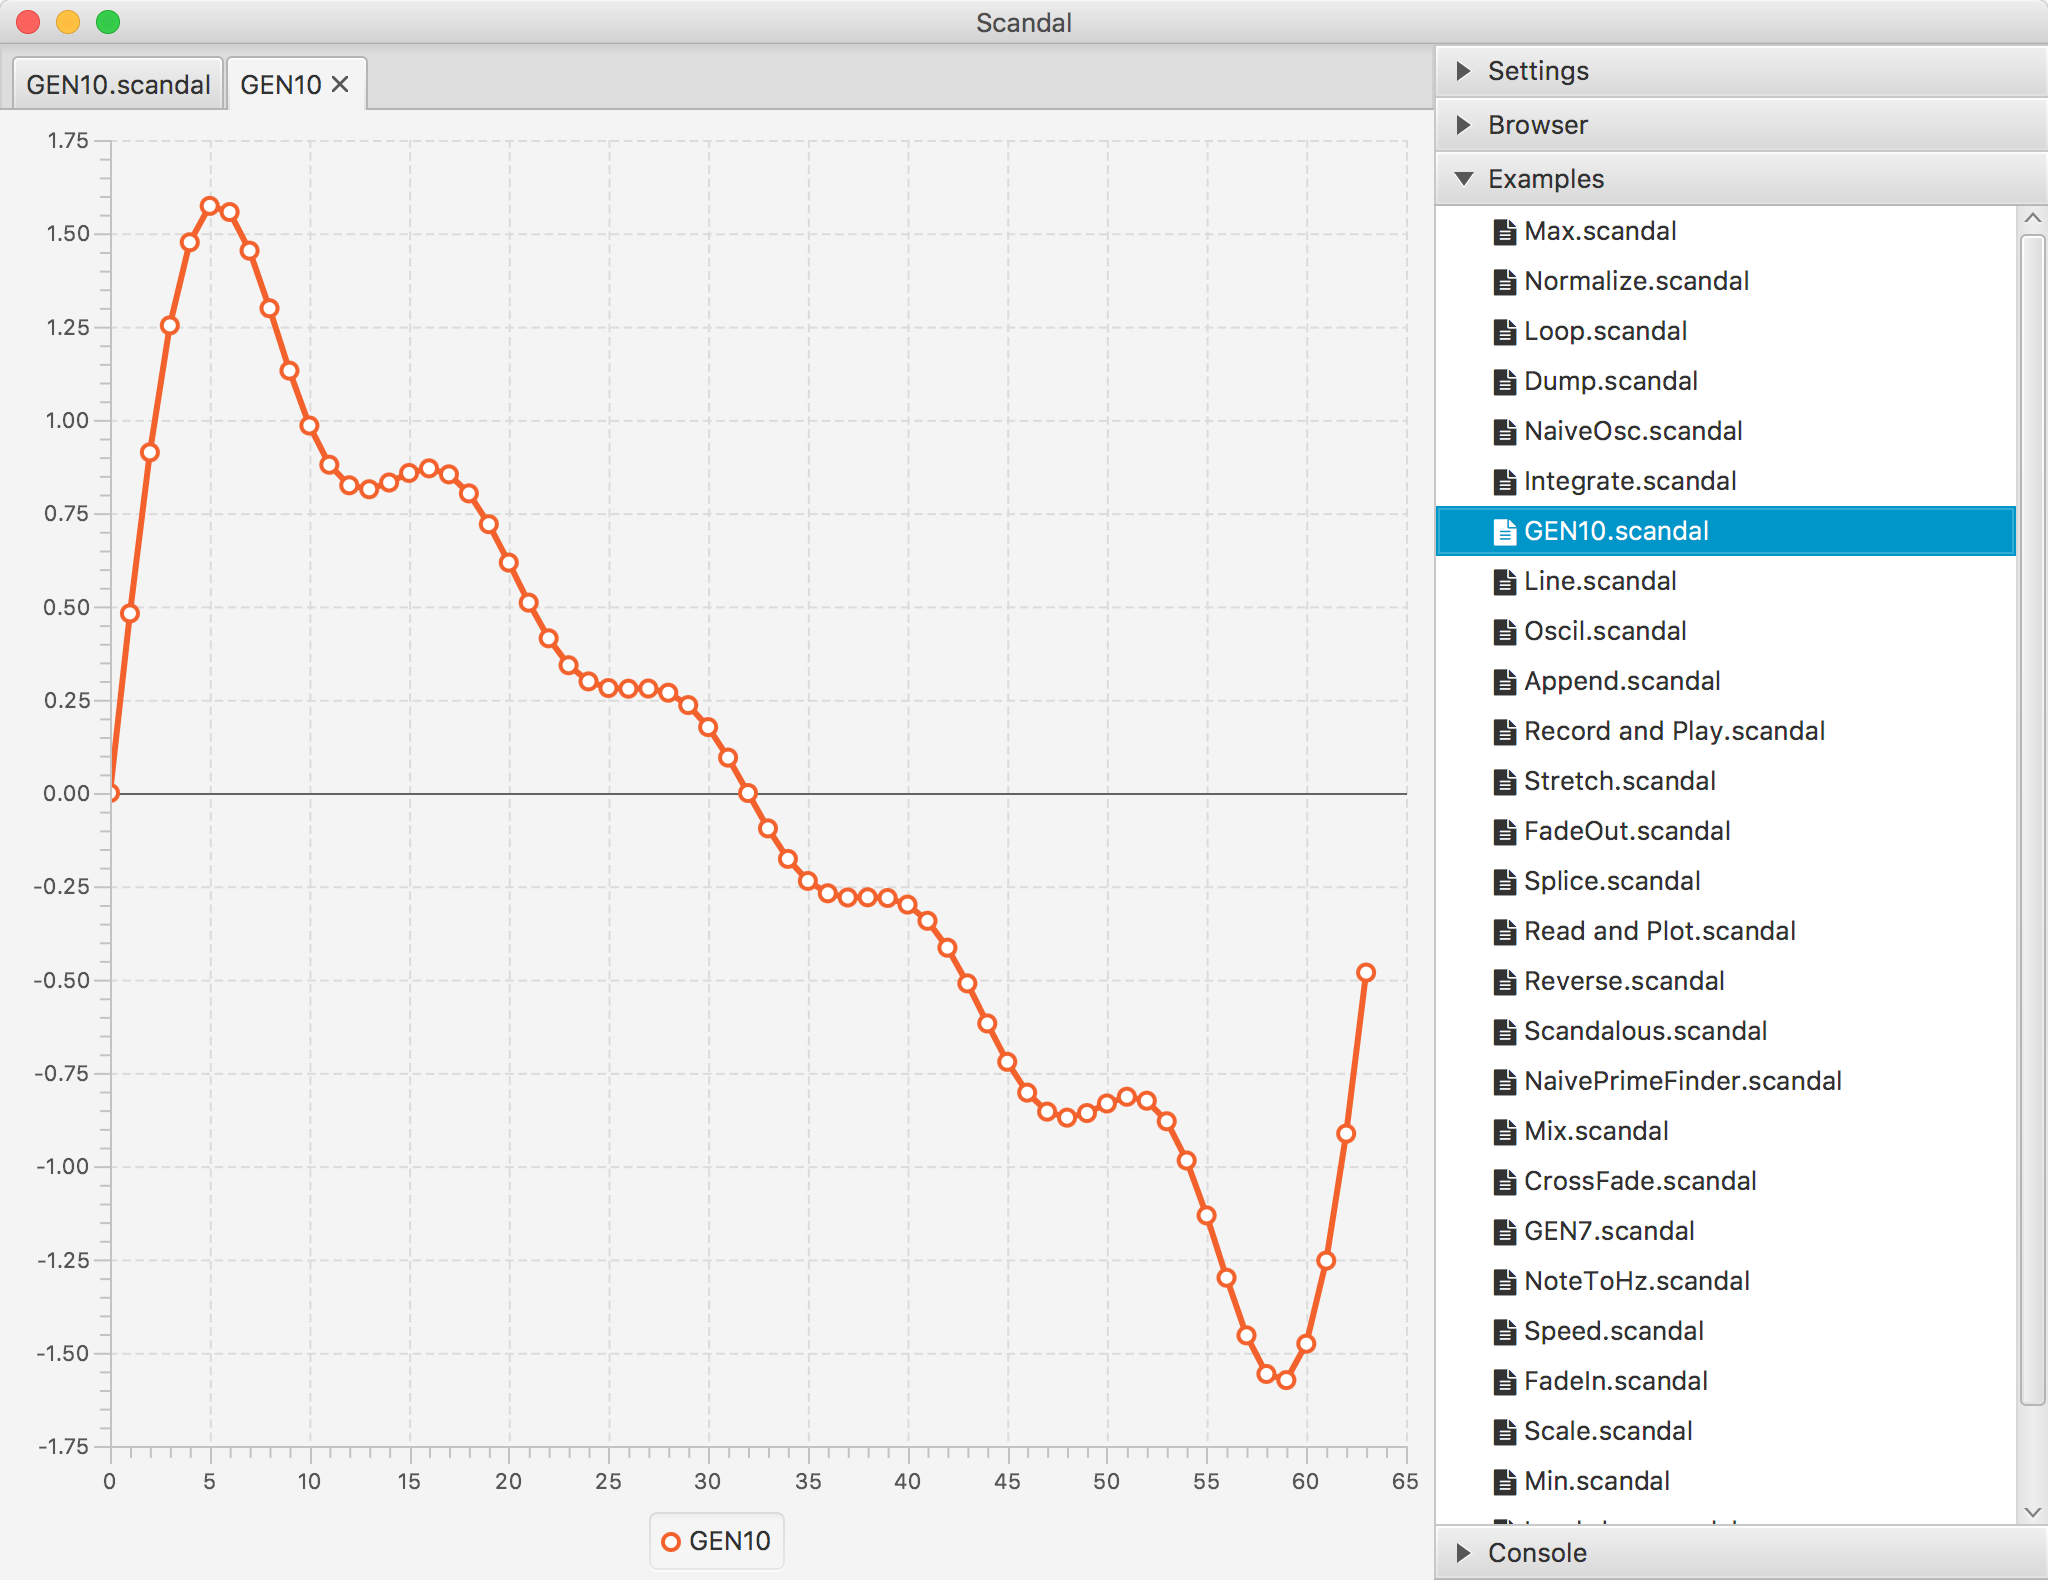
\includegraphics[width=4.5in]{img/plot}
	\caption[Plotting an array in \emph{Scandal}.]{Plotting an array in \emph{Scandal}.}
\end{figure}

\newpage Play statements take an array of audio samples and an integer number of channels, hence extend \il{Statement} by adding to it a second expression property. Parsing is done exactly the same way it is for plot statements, only there is one less expression to parse. The last type of framework statement in the language deals with saving a \emph{.wav} file to disk. Write statements take three arguments, namely the array containing audio samples, a string containing a path in the file system, and an integer number of channels. Parsing follows the exact same pattern found in other framework statements.

\section{Subclasses of Expression}

The abstract class \il{Expression} has a very diverse family of subclasses, and extends \il{Node} by adding to it three static methods. These methods are type converters and will be discussed in the context of lambda expressions. \il{Expression} neither implements \il{decorate} or \il{generate}, nor adds any properties to \il{Node}, hence remaining a fairly general type of node. Given their diversity, and the fact that often expressions come as binary sub-trees of the AST, expressions are by very far the most difficult construct in the language to parse. The \il{expression} routine in the parser, given below in Listing \ref{alg:expr}, works by always looking for operator tokens, then forming a binary expression whenever applicable. Hence, even when a simple literal expression is given, parsing thereof goes through several steps before being delegated to the specific parsing routine for that particular type of literal. In particular, parsing expressions begins by assuming the expression given is a binary expression containing a lowest-precedence comparison operator. Binary expressions extend \il{Expression} by overriding its abstract methods and adding to it three properties, namely a left-hand side expression, an operation token, and a right-hand expression. Below are the abstract syntax rules for expressions, wherein the rules for operators are the same as the concrete rules, except that instead of strings of characters, the abstract counterparts are given by instances of \il{Token}.

\begin{itemize}
	\item Expression := BinaryExpression $|$ DerivedExpression $|$ LiteralExpression
	\item Expression := ArrayExpression $|$ FrameworkExpression $|$ LambdaExpression
	\item BinaryExpression := Expression\_0 Operator Expression\_1
	\item Operator := ComparisonOperator $|$ SummandOperator $|$ FactorOperator
\end{itemize}

\begin{lstlisting}[language=Java,caption={Parsing Expressions.},label={alg:expr}]
public Expression expression() throws Exception {
	Token firstToken = token;
	Expression e0;
	Token operator;
	Expression e1;
	e0 = comparison();
	while (token.isComparison()) {
		operator = consume();
		e1 = comparison();
		e0 = new BinaryExpression(firstToken, e0, operator, e1);
	}
	return e0;
}
\end{lstlisting}

\begin{enumerate}
	\addtocounter{enumi}{2}
	\item Lines 3 to 5 declare two expressions, one for each node of the assumed binary sub-tree of the AST whose root is returned in line 12, and an operator token.
	\addtocounter{enumi}{2}
	\item Line 6 asks the \il{comparison} routine to provide the left-hand side expression, and line 7 tests in a while-loop to see whether the next token is a comparison operator. If so, the operator is stored and consumed in line 8, line 9 asks \il{comparison} for the right-hand side expression, and line 10 creates an instance of \il{BinaryExpression} with the two expressions. While the next token is still a comparison operator, the while-loop in line 7 keeps asking \il{comparison} for a new right-hand side, then substituting the current instance of \il{BinaryExpression} with another in which the left-hand side is the entire binary expression parsed last, and the right-hand side is the last expression returned from the \il{comparison} method. This method ensures binary expressions always associate equal-precedence operations from left to right.
	\addtocounter{enumi}{5}
	\item Finally, line 12 returns the left-hand side expression, which may or may not be a binary expression.
\end{enumerate}

The \il{comparison} routine does exactly the same \il{expression} does, only checking whether the operator token is at the precedence level of sums. Expressions are instantiated inside \il{comparison} by calling the \il{summand} routine. The \il{summand} routine, in turn, does also exactly the same as \il{expression} and \il{comparison}, only checking whether operator tokens are at the precedence level of products, which is the highest level of precedence among operator tokens in \emph{Scandal}. Expressions are instantiated inside \il{summand} by calling the \il{factor} routine. The latter returns a leaf in the binary tree by looking at the set FIRST(expression), similarly to how declarations and statements are parsed. Some factors, however, require more than one token of look-ahead, namely those that begin with an identifier, with the exception of simple identifier expressions. Inside the \il{factor} routine, whenever a token of kind \texttt{IDENT} is seen, the token next to it needs to be considered so it can be determined whether the factor should be parsed as an indexed array, a lambda application, a lambda composition, or a simple identifier expression. Since two tokens of look-ahead are necessary and enough to parse factors, no other construct in the language requires more than two tokens of look-ahead, constructs are parsed from left to right and leftmost-derived, it follows \emph{Scandal}'s grammar is LL(2).

\subsection{Derived and Literal Expressions}

Parsing derived expressions takes place in the \il{factor} method, as discussed above. For parenthesized expressions, \il{factor} simply looks for a left parenthesis, consumes it, recursively calls the \il{expression} method, then consumes the right parenthesis. Parenthesized expressions are crucial in order to resolve ambiguities, or force the compiler to construct a binary tree for an expression in a certain way. The expression $(1 + 1) / 2$ will be parsed differently than $1 + 1 / 2$, however the AST has no knowledge of parenthesis, it is the way in which binary expression trees are constructed that determines how they are evaluated. Therefore there are no abstract syntax rules for parenthesized expressions, since what they define is not a subtype, but a specific branching of a binary expression tree. Naturally, this tree may be trivial, or identical to a non-parenthesized tree. Such use of the parenthesized expression rule may have a purpose in improving readability of long mathematical expressions. Below are the abstract syntax rules for all derived expressions.

\begin{itemize}
	\item DerivedExpression := UnaryExpression $|$ IdentExpression
	\item UnaryExpression := (Token.\texttt{KW\_MINUS} $|$ Token.\texttt{KW\_NOT}) Expression
	\item IdentExpression := Token.\texttt{IDENT}
\end{itemize}

Unary expressions are parsed by consuming the operator token, then calling \il{expression} in the parser recursively. The \il{UnaryExpression} class extends \il{Node} by adding this referenced expression as a property. The operator is stored as the \il{firstToken} property, which is inherited from the superclass. Identifier expressions extend \il{Node} by adding to it a \il{declaration} property, which is naturally a subclass of \il{Declaration}. Parsing is done in the \il{factor} method, as well. Since the \emph{Scandal} grammar is LL(2), all of the cases in which an expression may begin with an \texttt{IDENT} token are first ruled out before an instance of \il{IdentExpression} is constructed.

All literal expressions extend \il{Expression} by adding no properties to it, since all that is needed is a value for the expression, which is in turn retrieved from the inherited \il{firstToken} property itself. For integers and floats, there is a risk the user will declare a number that is possibly too long. These cases are handled by the scanner at the earliest stage possible, and an informative compilation error is thrown if a bad number is given. In all literal expressions, types are assigned at their onset in the constructor, as type-inference mechanisms are unnecessary.

\subsection{Array Expressions}

For all but the \il{ArrayItemExpression} rule, array expressions are parsed in the \il{factor} method by looking at their first token. In the case of array item expressions, since FOLLOW(\texttt{IDENT}) = $\varepsilon$ $|$ \texttt{LBRACKET} $|$ \texttt{LPAREN} $|$ \texttt{DOT}, one more token of look-ahead is needed, namely a left brace. The other cases are those where a left parenthesis is seen, which correspond to lambda applications, and those in which a dot is seen, corresponding to lambda compositions. After consuming the first token, and possibly the second, parsing follows the same procedure as above, by calling the \il{expression} routine recursively, and abstracting away parenthesis, brackets, commas, and keywords. Below are the abstract rules for array expressions.

\begin{itemize}
	\item ArrayExpression := ArrayLitExpression $|$ ArrayItemExpression
	\item ArrayExpression := ArraySizeExpression $|$ NewArrayExpression
	\item ArrayLitExpression := (Expression)$^+$
	\item ArrayItemExpression := IdentExpression Expression
	\item ArraySizeExpression := Expression
	\item NewArrayExpression := Expression
\end{itemize}

Array literal expressions extend \il{Expression} by adding an \il{ArrayList} of expressions, and naturally overriding its abstract methods. Its type is set to \il{Types.ARRAY} in the constructor, similarly to how literal expressions are handled. Array item expressions extend \il{Expression} with two properties, namely an identifier expression that references the array, and an expression of type integer that stores the index information. Instead of storing an \il{IDENT} token, an \il{IdentExpression} is instantiated while constructing an \il{ArrayItemExpression}. The reason for that is to simplify decoration and code generation by delegating those tasks to the \il{IdentExpression} class, rather than repeating code inside \il{ArrayItemExpression}. Like with literal expressions, the type is always known to be \il{float}, hence set accordingly in the constructor. Array size expressions extend the superclass by including an expression of type \il{array}. Like before, the type is set to \il{int} in the constructor. The last type of array expression deals with creating a new array of zeros with a specified length. An instance of \il{NewArrayExpression} extends \il{Expression} by adding to it a \il{size} expression of integer type. Its type is too set to \il{array} in the constructor.

\subsection{Framework Expressions}

Parsing framework expressions is done in the \il{factor} method by simply looking at the first token at hand and constructing the appropriate subclass of \il{Expression}. Parenthesis, commas, and keywords are naturally all abstracted away. The abstract rules for framework expressions are omitted since they follow the usual pattern of listing all parameters to a framework routine as expressions. The simplest case of a framework expression is that of pi expressions. They extend \il{Expression} only by implementing its abstract methods. Like with literal expressions, its type is set to \il{float} right at construction, and decoration therefore does nothing. Cosine expressions are absolutely fundamental to audio signal processing, and are one of the cases where a pure \il{Scandal} implementation might not be worthwhile. They extend \il{Expression} by adding a \il{phase} property, which is a subclass of \il{Expression} of type \il{float}. Since cosine expressions always have type float in \emph{Scandal}, the type is set in the constructor. Power expressions provide a convenient way to compute exponential expressions, and extend \il{Expression} with two properties, namely \il{base} and \il{exponent}. Floor expressions are identical to cosine expressions, only naturally differing in functionality. Read expressions provide a hook to the audio engine's \il{framework.generators.WaveFile} class, whose main purpose is to parse the contents of a \emph{.wav} file in the file system and return them as an array of floats. \il{ReadExpression} extends the superclass by including two properties, a string \il{path}, and an integer \il{format}, the latter specifying a channel count. The \il{format} property is not overloaded, and accepts only integers. Finally, record expressions connect the DSL with the audio engine's \il{framework.generators.AudioTask} class. They extend \il{Expression} by adding a \il{duration} property, which has type integer but is overloaded to accept floats, as well.

\subsection{Parsing Lambda Expressions}

Parsing lambda literal expressions relies on looking at the first token at hand. Both variants feature a list of parameters separated by arrows, and each parameter is an instance of \il{ParamDeclaration}, hence begins with a type token. Since these are the only two types of expression that begin with a type token, the first token is enough to determine a lambda literal expression. While creating an array of parameter declarations, arrows are abstracted away until no more type tokens are seen. At this point, if a left brace is seen, a lambda block is instantiated and used to construct an instance of \il{LambdaLitBlock}. Otherwise, \il{expression} is called in the parser and the result used to instantiate a \il{LambdaLitExpression}. In fact, \il{LambdaLitBlock} is a subclass of \il{LambdaLitExpression}.

Parsing applications and compositions requires a second token of look-ahead, since both expressions begin with an identifier token. As previously discussed, indexed arrays and identifier expressions are the other two constructs that also begin with an identifier token. What distinguishes all four is the token that follows: indexed arrays are followed by a left bracket, lambda applications are followed by a left parenthesis, lambda compositions are followed by a dot, and identifier expressions are not followed by brackets, parenthesis, or dots. Once a parenthesis is found, the identifier is stored in an instance of \il{IdentExpression}, both parenthesis and all commas are abstracted away, and an instance of \il{LambdaAppExpression} is constructed with the identifier expression and a list of expressions, one for each given argument. If a dot is seen, however, all the subsequent dots are abstracted away while building a list of \il{IdentExpression}. When no more dots are seen, the next token may be a parenthesis or not. If so, an instance of \il{LambdaAppExpression} is used to construct a \il{LambdaCompExpression}, otherwise a null pointer is passed \emph{in lieu} of a \il{LambdaAppExpression} to the constructor of \il{LambdaCompExpression}. Below are the abstract syntax rules for lambda expressions.

\begin{itemize}
	\item LambdaExpression := LambdaLitExpression $|$ LambdaLitBlock
	\item LambdaExpression := LambdaAppExpression $|$ LambdaCompExpression
	\item LambdaLitExpression := ParamDeclaration$^+$ Expression
	\item LambdaLitBlock := ParamDeclaration$^+$ ReturnBlock
	\item ReturnBlock := (AssignmentDeclaration $|$ Statement)$^*$ Expression
	\item LambdaAppExpression := IdentExpression Expression$^+$
	\item LambdaCompExpression := IdentExpression$^+$
	\item LambdaCompExpression := IdentExpression$^+$ LambdaApp
\end{itemize}

The \il{LambdaLitExpression} class extends \il{Expression} by including a list of parameter declarations and a return expression, as seen above. In addition to that, it holds an integer property named \il{lambdaSlot}, which is used for naming the lambda in bytecode. Every lambda necessarily has at least one parameter, and necessarily returns a non-void expression. While constructing a lambda literal with expression, its type may be incorrectly inferred by the constructor of \il{Node} to be that of the expression's first token. Hence the expression type is set to \il{Types.LAMBDA} in the constructor of \il{LambdaLitExpression}. The \il{LambdaLitBlock} class is a type of lambda literal expressions in which an entire block of declarations and statements is featured before a return expression is given. Similarly to the superclass, the type of the expression is set to \il{Types.LAMBDA} already in the constructor. Lambda literals with blocks subclass \il{LambdaLitExpression} by adding to it a \il{block} property, that in turn is an instance of \il{ReturnBlock}. Return blocks extend \il{Block} by adding to \il{Block} a return expression property, and this return expression is used in the constructor of a \il{LambdaLitBlock} as an argument to construct the \il{LambdaLitExpression} super class.

An application of a lambda expression in \emph{Scandal} corresponds in the AST to an instance of the \il{LambdaAppExpression} class, which extends \il{Expression} by overriding its abstract methods and including four properties, namely an identifier expression called \il{lambda}, a list of expressions which are the arguments applied to this lambda, an immutable integer property named \il{count}, and a reference to an instance of \il{LambdaLitExpression} called \il{lambdaLit}. While constructing a lambda application expression, the size of the argument list is stored in the \il{count} property, as parameters might be added to this list in the decoration phase. The application type is also set to \il{Types.LAMBDA}, although that too might change if the application is not partial. Lambda compositions correspond to instances of \il{LambdaCompExpression}, which extend \il{Expression} by including two properties, an array of identifier expressions, and a lambda application expression. The latter can be null, as explained in the parsing process. If so, the type of the composition expression is set to \il{Types.LAMBDA} while constructing, otherwise setting a type is deferred until decoration.
\chapter{CHECKING TYPES AND DECORATING THE AST}

This chapter presents the type-checking rules for \emph{Scandal} along with the challenges involved in enforcing these rules in the language's \emph{Java} implementation. Although types are static in \emph{Scandal}, many productions are overloaded to accept types that can be easily cast to the required type. Moreover, operators are in their majority overloaded to accept mismatching types, in which case the rules defined in this chapter describe what types should be expected in return. Given that every node in the AST inherits from the \il{Node} abstract base class, type-checking takes place alongside other bookkeeping tasks in every node's \il{decorate} method. This routine is always called on a node by the node's parent. In particular, inside an instance of \il{Program}, type-checking is completely delegated to each node in its node array. More precisely, the \il{decorate} routine iterates over the node array and, for each node, calls \il{node.decorate}, passing along the symbol table instantiated by the compiler. Every direct child node of a program, in turn, delegates decoration of their child nodes, and with very few exceptions, delegation is the default behavior for AST decoration and type-checking.

\section{Decorating Declarations}

Decorating an instance of \il{AssignmentDeclaration} is a bit tricky. There are basically two tasks: checking that the variable is not being re-declared, and checking that the type of the given expression matches the type of the declaration. The declaration's type is set by the constructor of \il{Node} based on its first token. The \il{decorate} routine starts then by checking the top of the stack of symbol tables to see if there is no name clash, then inserts into the symbol table a key of \il{identToken.text} with value \il{this}. The next step is to assign a slot number to this variable, which is done by maintaining a property \il{slotCount} inside \il{SymbolTable}. The \il{slotNumber} property is set to the current slot count, and the latter is increased. A call to \il{expression.decorate} causes the expression to decorate itself and have a non-null type in most cases thereafter, except when the expression is an instance of \il{LambdaAppExpression}, in which case a roadblock in the type-checking process occurs. Listing \ref{alg:infer} provides a small snippet of \emph{Scandal} code to illustrate the situation.

\begin{lstlisting}[emph={lambda,float,return},emphstyle={\textbf},caption={Type inference in \emph{Scandal}.},label={alg:infer}]
lambda id = float x -> x
lambda higherOrder = float x -> lambda f -> {
	float val = f(x)
	return val
}
\end{lstlisting}

When a lambda expression in \emph{Scandal} has a parameter of type \il{lambda}, there is no mechanism in the language to tell what is the parameterized type of that lambda expression. The corresponding construction in \emph{Java} is an instance of the \il{Function} interface, which is a parameterized type. A lambda expression in \emph{Java} that takes a float and returns a float has type \il{Function<Float, Float>}, for example. It has been a design choice so far in \emph{Scandal} not to introduce parameterized types, and attempt instead at some yet crude type inference mechanism. In Listing \ref{alg:infer}, an instance of \il{ParamDeclaration} defines a variable \il{f} of type \il{lambda}. Inside the block, the mechanism of choice to in fact \emph{declare} what parameter types \il{f} has is through an assignment declaration or statement. In line 3, \il{x} is applied to \il{f} and the result stored in \il{val}. Since both \il{x} and \il{val} have type \il{float}, it can be inferred that \il{f} takes a single argument of type \il{float}, and returns also a float. Note that omitting line 3 and putting \il{return f(x)} instead would cause a compilation error, exactly because parameter types of a lambda expression cannot be inferred inside a lambda literal if there is no application thereof.

Given the discussion above, whenever an assignment declaration calls \il{expression.decorate}, and this expression happens to be an application of a lambda declared as a parameter of a lambda literal, instead of expecting the call to \il{expression.decorate} to define a type for the expression, the \il{AssignmentDeclaration} class itself needs to decorate the expression. The process is very simple: after calling \il{expression.decorate}, a check is made to determine if the expression is an instance of \il{LambdaAppExpression}. If so, the declaration of that application's \il{lambda} property is retrieved. If the declaration is an instance of \il{ParamDec}, then the expression at hand must be the application of a lambda declared as a parameter of a lambda literal expression, since parameter declarations only ever exist in the context of lambda literals. The \il{decorate} method then trust the programmer will make use of the lambda literal expression correctly, by applying to it a lambda expression that has the same parameter types as those inferred inside the block. If not, a runtime error will occur. Finally, the \il{expression} property will have to have a type, which is checked against the declaration type. Naturally, in the special case the expression was decorated for being an application of a lambda parameter, this test never fails. If it does, a compilation error is thrown.

\begin{itemize}
	\item AssignmentDeclaration:
		\begin{itemize}
			\item Must not be declared more than once in the same scope
			\item Type = Expression.type
		\end{itemize}
\end{itemize}

Decorating and type-checking field declarations is easier and involves checking all symbol table scopes to see if the variable is not being redeclared. Naturally, there is only ever one scope to check, the zeroth. The variable is then inserted into the symbol table with a key given by \il{identToken.text} and a value of \il{this}. A call to \il{expression.decorate} is made, after which the expression will be decorated with a non-null \il{type}, a property that is common to every node. Unlike \il{LambdaLitDeclaration}, in which the declaration and lambda always have the same type by construction, here a compilation error occurs if the program tries to store, say, a float into an integer field. This is not inherent to the JVM, however, which would in fact accept that a different type be stored in a local variable slot or field. In \emph{Scandal} this is illegal, hence decoration checks whether the expression's type is the same as the declaration's. The latter never needed to be decorated, and was set when the constructor of \il{Node} was called, since it could be inferred from the declaration's first token alone.

\begin{itemize}
	\item FieldDeclaration:
		\begin{itemize}
			\item Must be declared in the outermost scope
			\item Must not be declared more than once
			\item Type = Expression.type
		\end{itemize}
\end{itemize}

Lambda literal declarations have very different implementations of the \il{Node} abstract methods than those of its superclass \il{AssignmentDeclaration}, hence both \il{decorate} and \il{generate} are overridden. The bodies of these methods are substantially simpler than the superclass' implementation, given the restricted nature of this type. The \il{decorate} routine checks the entire stack of symbol tables to see whether the variable is not being redeclared, in which case an error is thrown. Checking only the topmost scope symbol table would work exactly the same, since lambda literal declarations are only allowed in the outermost scope, hence the stack only contains a single symbol table when the call to \il{decorate} is made. The next step is to insert the identifier into the symbol table, associating to it the instance of \il{LambdaLitDeclaration} at hand. Finally, calling \il{lambda.decorate} delegates decoration of the lambda expression to the \il{LambdaLitExpression} instance. The types of the declaration and expression are always equal to lambda, set in the respective constructors, and hence never need to be checked.

\begin{itemize}
	\item LambdaLitDeclaration:
		\begin{itemize}
			\item Must be declared in the outermost scope
			\item Must not be declared more than once
			\item Type = Types.\texttt{LAMBDA}
		\end{itemize}
\end{itemize}

When a lambda literal expression is decorated, a new scope in the symbol table is introduced, so that parameter names do not clash with local variables in the \emph{Java} class' \il{run} method. Thus, inside an instance of \il{ParamDeclaration}, the \il{decorate} method checks only the symbol table at the top of the stack of symbol tables to see whether any two parameters have the same identifier, in which case it throws a compilation error. If not, it inserts the identifier into the topmost scope of the symbol table, associating to the identifier the instance of \il{Declaration} at hand. Since parameter declarations are local variables inside a lambda body, they need to have the \il{slotNumber} property set so they can be accessed. This is accomplished, however, by the lambda literal expression class before the \il{decorate} method is called on a parameter declaration, as shall be seen momentarily.

\begin{itemize}
	\item ParamDeclaration:
		\begin{itemize}
			\item Must not be declared more than once
		\end{itemize}
\end{itemize}

\section{Decorating Statements}

Decoration of import statements begins by checking that the current scope number in the symbol table is zero, since the linker routine in the compiler only looks for imports in the outermost scope of each pre-compiled program. If not, an error is thrown. Next, a call to \il{expression.decorate} is made and, after the expression has been decorated with a type, a check is performed to see whether that is indeed a string, throwing an exception if not.

\begin{itemize}
	\item ImportStatement:
		\begin{itemize}
			\item Must be stated in the outermost scope
			\item Expression.type = Types.\texttt{STRING}
		\end{itemize}
\end{itemize}

Decorating assignment statements involves looking for a declaration value whose key corresponds to the identifier held in \il{firstToken.text}, starting from the innermost (topmost) scope, and descending to the bottom of the stack of symbol tables, as needed. Contrary to assignment declarations, if \emph{no} declaration is found, an error is thrown. Another check is made to determine if the declaration corresponds to a lambda literal expression, throwing an error if so. The latter are final fields in the \emph{Java} class, hence cannot be reassigned. Decoration of the \il{expression} property is delegated to the corresponding subclass of \il{Expression}, as usual. The exact same caveat with type inference in instances of \il{LambdaAppExpression} applies here, so a check is made to determine whether the given expression is a lambda application of a lambda parameter inside a return block. If so, the \il{AssignmentStatement} class decorates the lambda application expression with its declaration's type. All that is left is to check if the type of the declaration corresponds to the type of the expression, and an error is thrown if there is a mismatch.

\begin{itemize}
	\item AssignmentStatement:
		\begin{itemize}
			\item Must have been declared in some enclosing scope
			\item Cannot reassign lambda literals
			\item Declaration.Type = Expression.type
		\end{itemize}
\end{itemize}

Decoration of an indexed assignment statement is similar to the superclass in it checks the symbol table to see whether the identifier has been declared, throwing an error if not. In addition, a check must be made to determine if the declaration associated with the identifier has indeed type \il{array}, otherwise an error is also thrown. Decoration of the \il{index} property is delegated to the appropriate subclass of \il{Expression}, as usual. Contrary to most descendants of \emph{C}, however, \emph{Scandal} does allow arrays to be indexed by expressions of type \il{float}, in which case the integer part of the number is taken in the generation phase. Thus while checking the type of \il{index}, an error is thrown if is neither an integer nor a float. The \il{expression} property is decorated in a similar way, however here too care must be taken with higher-order functions. A check for those is performed exactly the same way it is in the superclass, decorating the \il{expression} property as needed. When decorating a lambda application inside a lambda block, the expression's type is naturally always set to \il{Types.FLOAT}. Similarly to the \il{index} property, the \il{expression} property is overloaded to accept integers, and in that case a conversion to float is performed in the generation phase before storing the expression's value.

\begin{itemize}
	\item IndexedAssignmentStatement:
		\begin{itemize}
			\item Must have been declared in some enclosing scope
			\item Declaration.Type = Types.\texttt{ARRAY}
			\item Expression\_0.type = Types.\texttt{INT} $|$ Types.\texttt{FLOAT}
			\item Expression\_1.type = Types.\texttt{INT} $|$ Types.\texttt{FLOAT}
		\end{itemize}
\end{itemize}

Decorating if and while-statements is identical. The \il{expression} property is asked to decorate itself, then checked to see whether it is of type boolean, an error being throw otherwise. After that, the block is asked to decorate itself. Decorating a block involves introducing a new scope by calling \il{symtab.enterScope}, asking each node in the block's \il{nodes} array to decorate itself, then calling \il{symtab.leaveScope}. Import statements are disallowed in blocks, since the compiler only ever looks for those in the zeroth scope, and so are lambda literals and fields. If a global variable declaration or an import statement is given to a block, neither the parser nor the block will take notice of it. The error will be thrown by the respective AST nodes upon decoration, when the node itself asks the symbol table for its current scope number, throwing an error if the latter is not zero.

\begin{itemize}
	\item IfStatement:
		\begin{itemize}
			\item Expression.type = Types.\texttt{BOOL}
		\end{itemize}
	\item WhileStatement:
		\begin{itemize}
			\item Expression.type = Types.\texttt{BOOL}
		\end{itemize}
\end{itemize}

Framework statements are all decorated in a similar fashion by delegating decoration to each parameter, then checking types. Decoration of a print statement asks the expression to decorate itself, after which a check is performed to determine if the expression's type is either \il{array} or \il{lambda}. In both cases an error is thrown. Decoration of a plot statement is accomplished simply by asking each expression to decorate itself, then type-checking the first to be a string, the second to be an array, and overloading the third to accept integers and floats. Decoration of play statements follows the same pattern, and requires that the first expression be an array, and the second be an integer. The same pattern applies to write statements, which require that the three expressions be of type array, string, and integer, respectively.

\begin{itemize}
	\item PrintStatement:
		\begin{itemize}
			\item Expression.type != Types.\texttt{ARRAY} $|$ Types.\texttt{LAMBDA}
		\end{itemize}
	\item PlotStatement:
		\begin{itemize}
			\item Expression\_0.type = Types.\texttt{STRING}
			\item Expression\_1.type = Types.\texttt{ARRAY}
			\item Expression\_2.type = Types.\texttt{INT} $|$ Types.\texttt{FLOAT}
		\end{itemize}
	\item PlayStatement:
		\begin{itemize}
			\item Expression\_0.type = Types.\texttt{ARRAY}
			\item Expression\_1.type = Types.\texttt{INT}
		\end{itemize}
	\item WriteStatement:
		\begin{itemize}
			\item Expression\_0.type = Types.\texttt{ARRAY}
			\item Expression\_1.type = Types.\texttt{STRING}
			\item Expression\_2.type = Types.\texttt{INT}
		\end{itemize}
\end{itemize}

\section{Decorating Expressions}

Decorating and generating binary expressions is somewhat involved, mostly due to the great variety of operators and their supported types. In addition, operators in \emph{Scandal} are overloaded to a certain extent, as to provide type polymorphism in binary expressions, which adds to the number of cases that must be considered while decorating and generating expressions, but also make the DSL more concise and readable. Decorating a binary expression begins with asking both expressions to decorate themselves, after which their types will be non-null. Given the binary-tree nature of these expressions, this is accomplished recursively, hence \il{decorate} may be calling on itself if one of the sub-expressions is a binary expression. For this reason, \il{decorate} needs to have a type before returning. In fact, almost all that is done inside \il{decorate} is to go over the different combinations of operators and expression types to determine what the overall type of the binary expression is. If given two expressions in any combination of integers or floats, arithmetic can be performed on those numbers. Note that arithmetic operators do not always have the same precedence amongst themselves. There are two sub-cases. If both expressions are of type integer, then the resulting binary expression is decorated with an integer type. Otherwise, if at least one of the expressions has type float, the whole binary expression will have type float. If instead any combination of integers, floats, or booleans is given, then logical or comparison operators can be used, remembering that booleans are implemented in bytecode as integers, and that logical operators also have different precedence levels. In both cases, the binary expression will be of type boolean. Before returning, the caveat of having applications of lambdas that were declared as parameters of another lambda must be considered. Given that there is no parameterization of types in \emph{Scandal}, these lambdas must be applied alone first in an assignment declaration or statement, which is the current inference mechanism for such parameterized types. So a check is performed on both expressions to see whether any of their declarations is a subclass of \il{ParamDeclaration}, and an error is thrown if that is the case. The very last thing we do while decorating a binary expression is to check if the binary expression's type is still null. If so, all tests above have failed. Since the binary expression must be decorated with a type, as mentioned above, an error is thrown whenever all type-checking cases fail.

\begin{itemize}
	\item BinaryExpression:
		\begin{itemize}
			\item ArithmeticOp := \texttt{MOD} $|$ \texttt{PLUS} $|$ \texttt{MINUS} $|$ \texttt{TIMES} $|$ \texttt{DIV}
			\item (\texttt{INT} $|$ \texttt{FLOAT}) ArithmeticOp (\texttt{INT} $|$ \texttt{FLOAT}) $\to$ \texttt{FLOAT}
			\item \texttt{INT} ArithmeticOp \texttt{INT} $\to$ \texttt{INT}
			\item ComparisonOp := \texttt{AND} $|$ \texttt{OR} $|$ \texttt{EQUAL} $|$ \texttt{NOTEQUAL} $|$ \texttt{LT} $|$ \texttt{LE} $|$ \texttt{GT} $|$ \texttt{GE}
			\item (\texttt{INT} $|$ \texttt{FLOAT} $|$ \texttt{BOOL}) ComparisonOp (\texttt{INT} $|$ \texttt{FLOAT} $|$ \texttt{BOOL}) $\to$ \texttt{BOOL}
		\end{itemize}
\end{itemize}

Decoration of unary expressions is simple, following the usual path of asking the expression property to decorate itself, after which type-checking proceeds as follows. If given a \texttt{MINUS}, and the expression is neither an integer not a float, an error is thrown. Else, if given a \texttt{NOT}, and the expression is not a boolean, an error is also thrown. Note that unary operators are not overloaded in \emph{Scandal}, and only apply to their specific types. Before returning, the unary expression is naturally decorated with the same type as the given expression. Type-checking identifier expressions is similar to assignment statements in that a check for a name that has already been declared is made, and an error is thrown if it has not. That is done by asking the symbol table for the declaration value associated to the given identifier key, after which the declaration is stored in the \il{declaration} property. The last step is to set the expression's type to be the same as the declaration's.

\begin{itemize}
	\item UnaryExpression:
		\begin{itemize}
			\item Token.\texttt{MINUS} Types.\texttt{INT} $\to$ Types.\texttt{INT}
			\item Token.\texttt{MINUS} Types.\texttt{FLOAT} $\to$ Types.\texttt{FLOAT}
			\item Token.\texttt{NOT} Types.\texttt{BOOL} $\to$ Types.\texttt{BOOL}
		\end{itemize}
	\item IdentExpression:
		\begin{itemize}
			\item Variable must have been declared in some enclosing scope
			\item Type = Declaration.type
		\end{itemize}
\end{itemize}

Decorating literal expressions is trivial. In all of them, \il{decorate} is overridden for being abstract, but nothing is done there, since all that is needed is to decorate the expression with a type, which is always known, hence done in each class' constructor.

\begin{itemize}
	\item IntLitExpression:
		\begin{itemize}
			\item Type = Types.\texttt{INT}
		\end{itemize}
	\item FloatLitExpression:
		\begin{itemize}
			\item Type = Types.\texttt{FLOAT}
		\end{itemize}
	\item BoolLitExpression:
		\begin{itemize}
			\item Type = Types.\texttt{BOOL}
		\end{itemize}
	\item StringLitExpression:
		\begin{itemize}
			\item Type = Types.\texttt{STRING}
		\end{itemize}
\end{itemize}

Decoration of array expressions follows the usual route. In all of them, the expression type is always known, hence set in the constructor. For array literal expressions, the \il{decorate} method iterates over the array of expressions, asking them to decorate themselves. For each of them, a check is made to determine that they have type integer or float, throwing an error otherwise. Ultimately, though, all values are cast to float when creating the array. Decoration of array item expressions asks the \il{array} property to decorate itself, then checks if it has type array, throwing an error if not. The same is done for the \il{index} property, only checking that it indeed has type integer or float. For array size expressions, decoration is done only by asking the \il{array} property to decorate itself, then checking it indeed has type \il{array}. For new array expressions, \il{decorate} asks the \il{size} expression to decorate itself, then checks it is either an integer or a float.

\begin{itemize}
	\item ArrayLitExpression:
		\begin{itemize}
			\item (Expression)$^+$.type = Types.\texttt{INT} $|$ Types.\texttt{FLOAT}
			\item Type = Types.\texttt{ARRAY}
		\end{itemize}
	\item ArrayItemExpression:
		\begin{itemize}
			\item Expression\_0.type = Types.\texttt{ARRAY}
			\item Expression\_1.type = Types.\texttt{INT} $|$ Types.\texttt{FLOAT}
			\item Type = Types.\texttt{FLOAT}
		\end{itemize}
	\item ArraySizeExpression:
		\begin{itemize}
			\item Expression.type = Types.\texttt{ARRAY}
			\item Type = Types.\texttt{INT}
		\end{itemize}
	\item NewArrayExpression:
		\begin{itemize}
			\item Expression.type = Types.\texttt{INT} $|$ Types.\texttt{FLOAT}
			\item Type = Types.\texttt{ARRAY}
		\end{itemize}
\end{itemize}

Framework expressions are also easily decorated, and type-checking arguments follows the usual pattern. For pi expressions, nothing is done inside \il{decorate}. Cosine expressions overload the \il{phase} property to accept integers and floats. In power expressions, both \il{base} and \il{exponent} properties are overloaded to accept integers and floats. Read expressions take a \il{format} argument that is of type integer and is not overloaded, similarly to play statements, which also have an integer-only property describing the channel count. Record expressions, on the other hand, do overload the \il{duration} property to accept integers as well as floats.

\begin{itemize}
	\item PiExpression:
		\begin{itemize}
			\item Type = Types.\texttt{FLOAT}
		\end{itemize}
	\item CosExpression:
		\begin{itemize}
			\item Expression.type = Types.\texttt{INT} $|$ Types.\texttt{FLOAT}
			\item Type = Types.\texttt{FLOAT}
		\end{itemize}
	\item PowExpression:
		\begin{itemize}
			\item Expression\_0.type = Types.\texttt{INT} $|$ Types.\texttt{FLOAT}
			\item Expression\_1.type = Types.\texttt{INT} $|$ Types.\texttt{FLOAT}
			\item Type = Types.\texttt{FLOAT}
		\end{itemize}
	\item FloorExpression:
		\begin{itemize}
			\item Expression.type = Types.\texttt{INT} $|$ Types.\texttt{FLOAT}
			\item Type = Types.\texttt{FLOAT}
		\end{itemize}
	\item ReadExpression:
		\begin{itemize}
			\item Expression\_0.type = Types.\texttt{STRING}
			\item Expression\_1.type = Types.\texttt{INT}
			\item Type = Types.\texttt{ARRAY}
		\end{itemize}
	\item RecordExpression:
		\begin{itemize}
			\item Expression.type = Types.\texttt{INT} $|$ Types.\texttt{FLOAT}
			\item Type = Types.\texttt{ARRAY}
		\end{itemize}
\end{itemize}

\section{Decorating Lambdas}

Decorating lambda literal expressions is not too complicated. Because new local variables are introduced with a lambda literal expression's list of parameters, decoration begins by pushing a new scope onto the symbol table stack. This allows names to be declared such that they will not clash with names already in the zeroth scope, however does not protect the lambda literal expression from \emph{seeing} the zeroth scope. Given that names in the bottom scope are local variables in the context of the \emph{Java} class' \il{run} method, and lambda bodies are scoped in an altogether different method within the same \emph{Java} class, any name declared in the zeroth scope is actually invisible to the lambda body. Of course, unless these names were declared as fields. After introducing a new scope, \il{decorate} iterates over the parameter list, assigning to each parameter a slot number, and asking each parameter to decorate itself. The parameter slot numbers are needed for local variables and are assigned sequentially from zero to the size of the list minus one. After that, the return expression is asked to decorate itself, and the symbol table is asked to leave the previously introduced scope. Finally, the \il{lambdaSlot} property is set to be equal to the symbol table's \il{lambdaCount} property, and the latter is incremented by the size of the parameter list. The reason for assigning a lambda number to each lambda literal is because lambda expressions are accessed by name in bytecode, and the naming convention is the word \emph{lambda} followed by a number. In addition, the \il{Function} interface naturally curries the parameters in a lambda expression and, per \emph{Scandal}'s design choice, parameters in a lambda have a traditional right-associative currying. This means there is a method body that responds to all parameters, another that responds to all but the first, and so on until the last method body that responds only to the very last, rightmost parameter. Therefore the leftmost body is associated to the \il{lambdaCount} slot, the one to its right is associated to the \il{lambdaCount}$ + 1$ slot, and the rightmost body is associated to the \il{lambdaCount} $+$ \il{params.size}$ - 1$ slot. In effect, that is exactly how these curried methods are accessed as partial applications, separately.

Decorating lambda literals with blocks is similar, but a bit more complicated than decorating lambda literals with expressions. As before, a new scope is introduced and \il{decorate} iterates over the parameter list, assigning parameters slot numbers and asking them to decorate themselves. Before asking the block to decorate itself, however, the fact that the block may contain declarations must be considered. Since declarations inside a return block are local variables to a method, they need slot numbers. The symbol table passed along has a running slot count for variables that are local to the \il{run} method, however, hence a temporary change to this value is needed. Every local variable inside the lambda block is assigned an incremental slot number that is offset by the number of arguments given in a lambda application. If, for example, a lambda has three parameters and three local variables, the parameters will have slot numbers ranging from zero to two, and the local variables will have slot numbers ranging from three to five. So the current slot count is stored in a local variable, changed to the size of the parameter list, the block is decorated, and finally the running slot count in the symbol table is set back to its previous state, using the value previously stored. After that, the topmost scope is popped, and the lambda count is increased in the symbol table by the size of the parameter list, similarly to lambda literals with expressions. Decoration of return blocks differ from the \il{Block} superclass in that they do not introduce a new scope, since that task is accomplished by the lambda literal that contains the return block. It also differs in that the return expression is asked to decorate itself.

Decorating a lambda application is not at all straightforward. The main complication is finding the declaration of a lambda literal that contains the body of the method to which the lambda application's list of arguments should be applied. In other words, the name reference held by the \il{lambda} property may not necessarily point to the declaration of a lambda literal, in which case a whole chain of name references needs to be unraveled until a declaration whose expression actually contains a method body is found. Decoration begins by asking \il{lambda}, which is an identifier expression, to decorate itself, after which it will be decorated with a declaration. A check is made to determine if the declaration is a parameter declaration, in which case decoration can go no further, since this is an application of a lambda that is a parameter of another lambda. In this case, the type of the application expression, as well as the parameterized type of its declaration, is inferred and set by an assignment declaration or statement, as discussed previously. All that is left to do then is to iterate over the parameter list, asking for each parameter to decorate itself, and return.

If the \il{lambda} declaration is not a parameter declaration, it might still not point to the declaration of a lambda literal, but at least it can be determined that it either lives inside \il{run}, or is a field. Decoration then traverses the AST from the application node backwards to its ancestors until a lambda literal is reached. There are basically three cases. In the first, the declaration of \il{lambda} points to an identifier expression. This case happens whenever a lambda expression is copied locally to a variable. The declaration then is set to point to the declaration of \emph{that} identifier expression, and traversal keeps looking, moving onto the previous ancestor. In the second case, the declaration points to a lambda composition. A lambda composition holds an entire list of identifier expressions, all of which may or may not point to the declaration of a lambda literal. In this case, there may be many parents to a node, but the very last is picked. Whatever lambda literal to which it ultimately points, must have a parameter list that matches this application's argument list, which is exactly what is needed in order to decorate this lambda application. If neither an identifier nor a composition, then the declaration must be pointing to another application. In this case, it cannot be known yet whether this application is a partial application, but it can be known for sure that the application to which the declaration points indeed is a partial application, for if it were total, this application could not exist, as there would be no more parameters to be fixed. But given this situation, it can be inferred that this application's argument list must be smaller that the parameter list of the lambda literal sought, since some partial application already fixed some of its parameters, and this application is a step further down the chain. Decoration then iterates over the argument list of the application to which the declaration points from right to left, that is, from its last down to its first element, and prepends to this application's list of arguments any of those arguments that its list does not yet contain. A sanity check is then performed to determine if some of these arguments have not already been added.

After traversing the AST without errors, the declaration pointer is guaranteed to have arrived at the declaration of a lambda literal, hence the latter's expression is stored in the \il{lambdaLit} property for further use during generation. Only at this point does decoration of the argument list actually begin. The \il{decorate} method iterates over the argument list, however the original argument list might have grown in the traversal process. That is why the size of the original list was stored in the \il{count} property, so \il{decorate} will restrict to \emph{only} the parameters that were originally in the list. That is accomplished by offsetting the iterator by the current argument list size minus its original size, which represents exactly the number of parameters that might have been added during traversal. By prepending arguments to the argument list, the latter now has been made the exact same size as the parameter list in \il{lambdaLit}, but there is no actual need to decorate arguments that were not meant for this particular application, hence why the list is offset. Moreover, the index of each original argument in the argument list now aligns properly with the corresponding parameters in the \il{lambdaLit} parameter list. Decoration then goes over the original parameters asking them to decorate themselves and checking that their types are the same as the types of the corresponding parameters in \il{lambdaLit}. Finally, a check is made to see if the type of this lambda application expression is indeed \il{lambda}. That is done by checking whether the current count of the argument list is the same as the parameter count in \il{lambdaLit}. If so, then the application has fixed all the parameters in \il{lambdaLit}, hence the type of the lambda application is set to the type of the \il{lambdaLit}'s return expression. If there are less arguments than \il{lambdaLit} has parameters, then this is a partial application, hence the current type definition is kept.

Decorating a lambda composition consists at the moment of just asking each composed lambda to decorate itself, then checking whether the \il{lambdaApp} property is null and, if not, asking it to decorate itself. The lambda application will in turn decorate its parameters and check that input types are correct. The last step is to set the type of the entire composition expression to the return type of its \il{lambdaApp}, if the latter is not null. This is an incomplete implementation, and the reasons for that shall be addressed in the following chapters.

\begin{itemize}
	\item LambdaLitExpression:
		\begin{itemize}
			\item Type = Types.\texttt{LAMBDA}
		\end{itemize}
	\item LambdaLitBlock:
		\begin{itemize}
			\item Type = Types.\texttt{LAMBDA}
		\end{itemize}
	\item LambdaAppExpression:
		\begin{itemize}
			\item Expression\_0.type = Types.\texttt{LAMBDA}
			\item The type of each argument must match the type of the corresponding parameter in the original lambda literal
			\item Type = Types.\texttt{LAMBDA} if the number of arguments given is less than the total number of parameters
			\item Type = the original lambda's return type if the number of arguments matches the total number of parameters
		\end{itemize}
	\item LambdaCompExpression:
		\begin{itemize}
			\item (Expression)$^+$.type = Types.\texttt{LAMBDA}
			\item The return type of each expression must match the input type of the next
			\item Argument types must match the first expression's input types
			\item Type = Types.\texttt{LAMBDA} if no arguments are given
			\item Type = the return type of the last expression if arguments are given
		\end{itemize}
\end{itemize}
\chapter{GENERATING TARGET CODE}

This chapter discusses the mechanisms necessary to translate a decorated \emph{Scandal} AST into \emph{Java} bytecode. This target language is characterized by running on the \emph{Java Virtual Machine}, a multi-platform interpreter and just-in-time compiler. Bytecode is written as text, but ultimately converted into a binary representation in order to facilitate execution by the JVM. In order to compile a \emph{Scandal} AST into bytecode text and binary representations, the \emph{Scandal} compiler makes use of a \emph{Java} library called \il{org.objectweb.asm}, or ASM for short. This library provides many facilities, including an IDE plug-in that takes a \emph{Java} class and displays its corresponding bytecode implementation, as well as the necessary ASM calls to generate that bytecode. In fact, this method represents most of the work flow in implementing \emph{Scandal}. The entire work flow is roughly:

\begin{enumerate}
	\item Make choices for the language's concrete syntax.
	\item Introduce new symbols to the \il{Token} and \il{Scanner} classes, as needed, and test.
	\item Write a corresponding AST class, parsing routine, and test.
	\item Describe type-checking rules, implement \il{decorate} inside the AST class, and test.
	\item Write \emph{Java} code with the same functionality, and copy its ASM plug-in output.
	\item Paste the ASM plug-in output inside the AST class' \il{generate} method, substituting names, constants, and method signatures by properties belonging to the AST class, make adjustments, and test.
\end{enumerate}

Often adjustments and optimizations are necessary, as the ASM plug-in output contains many unnecessary calls to its API. These are usually routines that add comments and line numbering to the bytecode class, but that can cause significant bloat in the compiler. Although not necessary, minor optimizations and code re-orderings are usually made, such as duplicating the top of the stack instead of making another method call, for example. Also, for every \emph{Scandal} type that is overloaded, a check is inserted with the necessary type conversion, as types are not overloaded in the JVM in general.

The \emph{Java Virtual Machine} is stack-based, that is, operands are stored in a stack data structure. Operations consist mainly of pushing operands onto the stack, then calling a method. If the method is void, it will pop from the stack the operands it takes as arguments and leave the stack in the same state it was before those operands were pushed. If the method returns something then it will leave, in addition, a result on top of the stack, that is, after popping its required arguments. Stacks in the JMV are further bundled into entire frames, which contain data and local variables the stack can access. Bytecode is oblivious to most details pertaining to the implementation of frames, except for providing the frame's local variable count and maximum stack height. Naturally, these \emph{details} are fundamental for memory allocation in the JVM. Fortunately, computing these values is delegated entirely to the ASM library, as previously discussed.

\section{Generating a Program}

Generating bytecode in the \il{Program} class is a lot more complex than the corresponding decoration phase, since the overall structure for the entire underlying \emph{Java} class needs to be provided. This global task is accomplished inside the \il{generate} method by creating an instance of \il{org.objectweb.asm.ClassWriter}. The latter, which is stored locally in a property called \il{cw}, manages the creation of the \emph{Java} class itself, including the generation of the byte array used to instantiate and run the \emph{Scandal} program. In particular, the JRE is set to version 1.8, access to the class is made \il{public}, and the class is defined as a subclass of \il{java.lang.Object} that implements the \il{java.lang.Runnable} interface. This is all accomplished by calls to the ASM API, which manages writing a bytecode class with the appropriate instructions. Next, three instances of \il{org.objectweb.asm.MethodVisitor} are acquired by calling \il{cw.visitMethod}, one for each method in the \emph{Java} class. The methods are namely \il{init}, \il{run}, and \il{main}.

The \il{init} method basically goes through the node array and, if the particular node is an instance of \il{LambdaLitDeclaration}, a call is made to \il{node.generate}, passing the appropriate instance of \il{MethodVisitor} and the compiler's symbol table as arguments. What the \il{generate} method does inside a \il{LambdaLitDeclaration} is somewhat complicated, and its explanation deferred to the moment the \il{LambdaLitExpression} class is discussed. Before visiting \il{run}, \il{generate} goes once again over all nodes in the node array and, if they are either an instance of \il{LambdaLitDeclaration} or an instance of \il{FieldDeclaration}, it calls \il{cw.visitField}. The latter method creates fields in the \emhp{Java} class, which correspond to global variables in the \emph{Scandal} program. Every field is marked as \il{static}, since no use is made in \emph{Scandal} of \emph{Java}'s object-oriented paradigm.

In addition, lambda fields are marked as \il{final}, as previously discussed, and \il{cw} is passed along to the instances of \il{LambdaLitExpression} for which field declarations are being created, asking them to create method bodies for their respective lambda literal expressions. This is accomplished inside each lambda literal expression by an overloaded \il{generate} method, which takes, instead of a \il{MethodWriter}, an instance of \il{ClassWriter}, namely \il{cw}. Each lambda literal expression uses \il{cw} to create its own \il{MethodWriter}, which will write the lambda's corresponding method to the \emph{Java} class. These instances of \il{LambdaLitExpression} are accessed through the corresponding \il{lambda} property inside a \il{LambdaLitDeclaration} class, and the particularities of creating method bodies for lambdas will be discussed momentarily.

The next step is to add a body for the \emph{Java} class' \il{run} method. To do so, \il{generate} goes yet once more over the array of nodes, and this time it generates any node that is \emph{not} an instance of \il{LambdaLitDeclaration}, for obvious reasons. It does, however, visit instances of \il{FieldDeclaration}, since \il{cw.visitField} only created the fields, but never assigned any values to them. Since unassigned declarations are only allowed in \emph{Scandal} when declaring lambda parameters, there is always some value to assign to those fields at initialization, and \il{generate} inside \il{FieldDeclaration} takes care of exactly that. Finally, \il{generate} visits the \il{main} method in the \emph{Java} class, which is shown in Listing \ref{alg:main}.

\begin{lstlisting}[language=Java,caption={Using the ASM framework to construct a \il{main} method.},label={alg:main}]
private void addMain(ClassWriter cw, SymbolTable symtab) {
	MethodVisitor mv = cw.visitMethod(ACC_PUBLIC + ACC_STATIC, "main",
		"([Ljava/lang/String;)V", null, null);
	mv.visitTypeInsn(NEW, symtab.className);
	mv.visitInsn(DUP);
	mv.visitMethodInsn(INVOKESPECIAL, symtab.className,"<init>","()V",false);
	mv.visitMethodInsn(INVOKEVIRTUAL, symtab.className, "run", "()V", false);
	mv.visitInsn(RETURN);
	mv.visitMaxs(0, 0);
}
\end{lstlisting}

\begin{enumerate}
	\addtocounter{enumi}{1}
	\item This is the standard \il{main} method in \emph{Java}, which is always \il{public} and \il{static}, takes an array of strings, and returns nothing. The bytecode syntax for arrays is that of a left bracket, followed by the type. Line 2 uses \il{cw} to create an instance of \il{MethodVisitor}, namely \il{mv}, with exactly these properties. Bytecode syntax for method signatures is given by a parenthesized list of argument types, followed by a return type. Hence a \il{void} method that takes a \il{String[]} in \emph{Java} becomes \il{([Ljava/lang/String;)V}, where the left bracket means an array of whatever type follows, and the colon separates arguments. Naturally, \il{java/lang/String} is a string, and \il{V} stands for the \il{void} type.
	\addtocounter{enumi}{1}
	\item The JVM is stack-based, so line 4 creates a new instance of the \emph{Java} class, whose name is stored in the compiler's symbol table, and the result is left on top of the JVM stack.
	\item Line 5 duplicates whatever is on top of the stack, since the newly created \emph{Java} class will be needed twice, namely for a call on it to \il{init}, and another on \il{run}. These two calls are made in lines 6 and 7, respectively. Notice both method signatures take no arguments and return nothing, hence are equivalent to \il{()V} in bytecode.
	\addtocounter{enumi}{2}
	\item Finally, a return statement is added to the \il{main} method's body, which is omitted in void \emph{Java} methods, but required in bytecode.
	\item A bytecode method requires that the maximum number of elements the stack will have, as well as the total number of local variables in the method be computed. ASM will do that automatically by passing \il{ClassWriter.COMPUTE_FRAMES} as an argument to the constructor of \il{ClassWriter}. The two arguments to \il{mv.visitMaxs} are the maximum stack size, and the total number of local variables. Zeros are passed here since ASM is computing them later, but the call must be made nonetheless.
\end{enumerate}

\section{Generating Declarations}

Overriding the \il{generate} method inside an assignment declaration is straightforward, and consists of making a call to \il{expression.generate}, which causes the expression value to be left on top of the JVM stack, after which a switch statement determines the expression type, and uses the appropriate JVM instruction to store the variable. For integers and booleans it uses \il{ISTORE}, for floats it uses \il{FSTORE}, and for all other types in \emph{Scandal} it uses \il{ASTORE}. Similarly, the \il{generate} method in lambda literal declarations calls \il{lambda.generate}, which causes a lambda literal expression to be left on top of the JVM stack. This expression is then bound to the \il{identToken.text} property using the \il{PUTSTATIC} bytecode instruction. The overridden \il{generate} method in field declarations is identical to that of \il{LambdaLitDeclaration}. In the \il{generate} method, parameter declarations do nothing, since there is no value that can be bound to the declaration's identifier at the moment. Naturally, these values will exist in the context of a lambda application.

\section{Generating Statements}

Even though import statements belong to the AST, no bytecode is ever generated for them. The \il{generate} method still needs to be implemented for being abstract, but simply nothing is done there. The \il{generate} method for assignment statements, on the other hand, is somewhat more complicated, since the \il{Function} interface in \emph{Java} only handles classes and not primitive types. This restriction applies in \emph{Scandal} to integers, floats, and booleans, which are implemented as primitives, and must therefore be wrapped in a \emph{Java} class, namely \il{Integer}, \il{Float}, and \il{Boolean}, in order to be assigned to parameters in a lambda literal expression. The other three types in \il{Scandal}, namely strings, arrays, and lambdas, all correspond to class types in \emph{Java}, hence do not require any conversion. Before assigning to any variable, an expression value is always left on top of the JVM stack. Whenever assigning to a parameter variable inside a lambda literal expression or block, if the expression's type corresponds to a primitive type in \emph{Scandal}, this primitive sitting on top of the JVM stack is wrapped into the appropriate \emph{Java} class. That is done by testing whether the \il{declaration} property inside the assignment statement class is an instance of \il{ParamDeclaration}, which immediately tells the variable is a parameter to a lambda. Otherwise, a test is performed to determine if the \il{declaration} is an instance of \il{FieldDeclaration}, in which case the \il{PUTSTATIC} bytecode instruction is used to assign the expression to the variable. If both tests fail, then the variable must be local, either in the context of \il{run} or local to a lambda body, hence the appropriate store call is made based on the variable type, similarly to assignment declarations. Here a slot number is needed, but that is conveniently stored in the \il{declaration} property, which computed it during its decoration phase.

Generating an indexed assignment statement is done a little differently from the \il{AssignmentStatement} superclass in it involves loading the array first on top of the JVM stack, which is done by asking the \il{declaration} property for a slot number and calling \il{ALOAD}. After that, the \il{index} property is asked to generate itself. If the index is a float, the \il{F2I} instruction is called, which effectively pops the float and pushes its integer part on top of the JVM stack. Similarly, the \il{expression} property is asked to generate itself and, if needed, converted to float by calling the \il{I2F} JVM instruction. Finally, the \il{FASTORE} instruction is used to assign the value on top of the stack to the array at the desired index, eventually popping the three topmost elements from the JVM stack. The \il{generate} method naturally differs between both types of conditional statement. The entire process of generating an if-statement is described in Listing \ref{alg:if}.

\begin{lstlisting}[language=Java,caption={Generating If-Statements.},label={alg:if}]
public void generate(MethodVisitor mv, SymbolTable symtab) throws Exception {
	expression.generate(mv, symtab);
	mv.visitInsn(ICONST_1);
	Label label = new Label();
	mv.visitJumpInsn(IF_ICMPNE, label);
	block.generate(mv, symtab);
	mv.visitLabel(label);
}
\end{lstlisting}

\begin{enumerate}
	\addtocounter{enumi}{1}
	\item Line 2 asks the expression to generate itself, after which its value will be left on top of the JVM stack.
	\item Line 3 loads a constant of value true, given by the \il{ICONST_1} instruction, on top of the stack. Interestingly, integer constants are used in the bytecode implementation of booleans, but not in \emph{Java}. Nor in \il{Scandal}, mostly for clarity.
	\item An instance of \il{org.objectweb.asm.Label} is then created which, upon a call to \il{mv.visitLabel} in line 7, creates a bytecode label instruction.
	\item Before visiting the label, though, both elements on top of the stack are compared by making a call to an \il{IF_CMPNE} jump, and giving it the label just created as an argument. When called, it will pop both topmost elements and jump to the label if these elements are not equal. Since at least one of them has value true, namely the one in line 3, the jump is performed only if the condition is false.
	\item What is jumped over is exactly the contents of the block, thus the block is generated in line 6 still before the label is visited. Generating a block requires simply iterating over its \il{nodes} array, asking each node to generate itself.
\end{enumerate}

Generating while-loops is analogous, but requires two labels, since the loop keeps jumping back to the first label while the condition is true. Naturally, the first label is visited first, to establish that jump location. Then, the expression and a constant of value true are pushed, followed by a call to \il{IF_CMPNE}, as with if-statements, passing as an argument the second label, which is yet to be visited. Next, the block is visited and a \il{GOTO} instruction is added, giving it the first label as an argument, which causes the condition to be re-evaluated. If still true, the block is repeated. If not, a jump to the second label is performed, whose visit is the last step in generating a while-loop. The actual bytecode implementation often involves more instructions. Generation thereof is gladly delegated to the ASM library.

Generating print statements depends on whether the \emph{Scandal} program is running inside the IDE, or in the command line. A call to \il{Platform.isFxApplicationThread} is made to check. If running on the command line, \il{mv} is used to load \il{System.out}, the expression is asked to generate itself on top of it, and finally \il{mv} is used again to call \il{println} on \il{System.out}. If running on the IDE, \il{mv} is used to load \il{language.ide.MainView.console}, which is an instance of \il{javafx.scene.control.TextArea}. The top of the stack is then duplicated, for reasons explained momentarily. The expression is then generated on top of that, and a test is made to see if the expression is not of type \il{string}, in which case a call is made to \il{String.valueOf}, since \il{TextArea} can only append to its contents a value of type \il{java.lang.String}. To actually append the string to whatever the console is displaying at the moment, a call is made to \il{TextArea.appendText}, which pops the two topmost elements, namely the expression and the duplication of the console. A new-line character is then pushed, and a call is made to \il{TextArea.appendText}, in order to create a line break. This causes the top of the stack to be popped twice, hence why the console was duplicated.

The generation phase for plot statements consists of checking, similarly to print statements, whether the program is running on the IDE. If not, no bytecode is generated, hence one cannot see plots when running a \emph{Scandal} program from the command line. Otherwise, we \il{mv} is used to push a new instance of \il{language.ide.PlotTab}, and all three expressions are pushed on top of it. If the last expression has type float, the \il{F2I} instruction is used, and finally \il{init} is called on the \il{PlotTab}, causing it to be displayed on the IDE's main view.

Like before, generation of play statements involves checking whether the program is running inside the IDE. If not, \il{mv} is used to push a new instance of \il{AudioTask} onto the stack, which is duplicates, since it need to be used twice. A call to \il{init} on the \il{AudioTask} follows, which pops the topmost of the two. Both expressions are then generated, and a call to \il{play} on the \il{AudioTask} is made. If the program is running on the IDE, however, a new instance of \il{language.ide.WaveTab} is pushed instead. Next, a string is pushed containing the class name, which the symbol table holds, both expressions are generated, and call is made to \il{init} on the \il{WaveTab}. The string containing the class name is used as the tab's label. The \il{WaveTab} class in the IDE is a subclass of \il{PlotTab}, and displays a plot of the array of samples, decimated to 1000 samples, in addition to playing it back, hence there one never needs to plot \il{and} play in a \emph{Scandal} program. The code-generation routine in write statements uses \il{mv} to push a new instance of \il{framework.generators.AudioTask}, which is duplicated. After calling \il{init} on the \il{AudioTask}, all expressions are pushed and \il{export} is called on \il{AudioTask}, which effectively saves the audio buffer as a \emph{.wav} at the specified path.

\section{Generating Expressions}

Generating binary expressions is unsurprisingly involved, given that operators are \emph{not} overloaded in bytecode at all, hence a fair amount of work is needed to guarantee operators are matched with compatible types. The basic mechanism is to load the left expression, then create a switch case for each kind of operator. The procedure for all arithmetic operators is very similar. After pushing the left expression, a check is made to see if the binary expression has type float. If so, then at least one of the expressions must have type float. So while the left expression is still on top of the stack, \il{generate} checks if it is \emph{not} a float, and if so calls the \il{I2F} instruction. Next, the right expression is pushed and the same check is performed. The last step is to call the appropriate JVM instruction to deal with the float case of the arithmetic operator at hand. If, on the other hand, the binary expression has integer type, then necessarily \emph{both} expressions also have integer type, so \il{generate} just pushes the second expression and calls the appropriate JVM instruction. In the cases where the operation involves a logical operator, the JVM can only perform those operations on integers, including naturally integer representations of booleans. So here the left expression is loaded and cast to integer if it is a float, the same for the right expression, and the logical operator's instruction is called. Comparison operators are more tricky, since \il{generate} cannot count on the overall type of the binary expression to make necessary conversions, and the JVM does have separate instructions for integers and floats, requiring both sides to have the same type. Every binary expression whose operator is a comparison has type boolean, but still, JVM instructions are not overloaded. Hence the top of the stack needs to have agreeing types before a particular instruction is called. However, observing that after calling the operator instruction, the top of the stack is always left with an expression of type boolean, instead of testing every possible case, \il{generate} casts both expressions to float, as needed, and only resorts to float comparisons.

Generation of unary expressions starts by pushing the expression on top of the stack. It then looks at the expression type and covers three cases. If it is an integer, then from type-checking it is only possible that the given operator is a \texttt{MINUS}, hence \il{generate} calls the \il{INEG} instruction. The same applies for floats, only that the \il{FNEG} instruction is called. Code generation is surprisingly more involved for the boolean case. If given a boolean expression, then it needs to be negated. That is accomplished by creating two labels, visiting an \il{IFEQ} jump instruction, and giving it the first label as an argument, which causes the top of the stack to be popped. If the stack contained a zero, that is, if the expression evaluates to false, then a jump to the first label is performed, where a \il{ICONST_1} is pushed onto the stack. If the stack contained a true instead, then a \il{ICONST_0} is pushed, and \il{generate} visits a \il{GOTO} jump, giving it as an argument the second label. At the second label location, nothing is really done, and \il{generate} just leaves the false value on top of the stack and returns.

Generating identifier expressions resorts to three cases. The first case is when the declared variable is a field, which is known from the \il{isField} property every declaration contains. If so, \il{generate} use \il{mv} to push the value associated with the field's name. The second case deals with the possibility that the variable is a parameter inside a lambda, which happens whenever the \il{declaration} property is an instance of \il{ParamDeclaration}. If so, then surely the value of the expression is not a primitive, since the \il{Function} interface requires values to be passed as classes, as discussed previously. The \il{generate} method then does two things, namely it uses \il{ALOD} to push the expression's value, then calls \il{Expression.getTypeValue}, a static method that converts from classes left on top of the stack to their primitive values. Naturally, this only applies to integers, floats, and booleans. If neither a field, nor a parameter, then \il{generate} loads the variable normally. For integers and booleans, it uses \il{ILOAD}, for floats \il{FLOAD}, and for all other types it uses \il{ALOAD}. Except for fields, a slot number is always needed to load variables, which is retrieved from the \il{declaration} property every identifier expression contains.

Code generation of literal expressions is easy. For integers and floats, \il{generate} calls respectively \il{Integer.parseInt} and \il{Float.parseFloat}, using the result as an argument to \il{mv.visitLdcInsn}, which effectively pushes the value onto the stack. There is no risk of finding bad numbers here, as a check has already been made during scanning. For booleans, \il{generate} tests the given keyword, and loads the appropriate constant, whereas for strings, it uses \il{mv} to load the \il{firstToken.text} property directly.

Generating array literal expressions requires constructing the array, element by element, on the JVM stack. To do so, \il{generate} uses \il{mv} to push the size of the list of floats onto the stack, then calls the \il{NEWARRAY} instruction with a \il{T_FLOAT} argument. It then iterates over the list of floats and, for each expression, duplicates the top of the stack, pushes an index value onto the stack, asks the expression to generate itself, converting it to float as needed, and finally calls the \il{FASTORE} instruction, which stores the expression's value onto the new array at the specified index. At the end of the each iteration, the call to \il{FASTORE} pops the topmost two elements, hence at the end of the entire process, \il{generate} effectively leaves the filled-up array on top of the stack. Generation of array item expressions asks the \il{array} property to push itself onto the stack, then asks the \il{index} property to do the same. If the index has type float, \il{generate} calls \il{F2I}, as usual. Finally, \il{generate} uses \il{mv} to call \il{FALOAD}, leaving a float on top of the stack. Generation of array size expressions is also easy, asking the \il{array} property to load itself, then using \il{mv} to call the \il{ARRAYLENGTH} instruction. Code generation of new array expressions loads the \il{size} property on top of the stack and converts it to integer, as needed, finally calling the \il{NEWARRAY} instruction with a \il{T_FLOAT} argument, similarly to array literal expressions.

Code generation of pi expressions is trivial, with \il{generate} simply asking \il{mv} to load \emph{Java}'s \il{Math.PI} on top of the stack. Generation of cosine expressions asks the \il{phase} property to leave a value on top of the stack, then converts it to double using either the \il{F2D} or the \il{I2D} instruction, since the method signature for \emph{Java}'s \il{Math.cos} takes a double and returns a double. It then uses \il{mv} to invoke \il{Math.cos}, finally casting the result back to float using \il{D2F}. For power expressions, the method signature for \il{Math.pow} in \il{Java} takes two doubles and returns one, so \il{generate} converts back and forth, similarly to what is done in cosine expressions. Floor expressions follow the same pattern, only by invoking \emph{Java}'s \il{Math.floor} method instead. For write expressions, code generation asks \il{mv} to create a new instance of \il{WaveFile}, which is duplicated. It then generates the \il{path} property and calls \il{init} on \il{WaveFile}. Next, \il{generate} pushes the \il{format} property and calls \il{WaveFile.get}, which leaves an array of floats on top of the stack. Code generation of record expressions is very similar to read expressions, where \il{generate} instantiates an \il{AudioTask}, duplicates it, and calls \il{init}. It the pushes the \il{duration} property onto the stack, which is given in milliseconds, and casts it to integer, as needed, finally calling \il{AudioTask.record}. The latter will block execution of the \il{Scandal} thread for the entire \il{duration}, capture input from the preferred audio input device in \il{Settings}, then leave an array of floats on top of JVM the stack.

\section{Generating Lambdas}

Code generation of lambda literal expressions is a lot more involved than expressions in general, and accomplished in two stages. In the first stage, an instance of \il{Program} calls the \il{generate} method overridden from \il{Node}, giving it as an argument the instance of \il{MethodVisitor} associated with the \emph{Java} class' \il{init} method. The purpose of the code generated inside \il{init} is to associate the lambda declared as a field with a method body. Every lambda literal implements the \il{Function} interface, which is a \emph{Java} functional interface, so called whenever they comprise a single abstract method, and any number of methods containing bodies. Thus an object that implements the \il{Function} interface needs to be instantiated for each lambda literal declared. This object will in turn implement the interface's abstract method, which is matched to the expression or block held inside each \il{LambdaLitExpression}. This object can thereafter be treated as a variable. Whenever a lambda expression is applied arguments or composed with other lambda expressions, the JVM is basically calling methods on this class. Note that the one abstract interface method is however a static and synthetic method of the class that \emph{defines} the implementor of the functional interface, and not part of the implementing object itself. For this reason, type-checking inside the JVM is deferred until runtime, hence \il{generate} uses the \il{INVOKEDYNAMIC} instruction to call \il{java.lang.invoke.LambdaMetafactory}, which does all the heavy lifting, instead of doing all the above wiring explicitly. In \emph{Java}, lambda expressions are essentially syntactic sugar for objects that implement functional interfaces.

Inside the first stage of code generation, a string is formed containing the lambda's method signature. This method signature consists of a single input type and a return type. The reason for a single input parameter, despite the size of the parameter list, is the right-associated currying of lambda expressions described above, in which a function of $n$ variables that returns a value is seen as a function of one variable that returns a function of $n - 1$ variables, and so on until a function of one variable that returns a value, when the last variable is reached. It follows the required method signature always has as input type the type of its very first argument, always given as a \emph{Java} class, as \il{Function} accepts no primitive types. The return type depends on the size of the argument list, naturally. If only one argument is given, then the expression's return type is the type of the return expression, otherwise the return type is \il{java.util.function.Function}. Having formed this string, \il{generate} uses it as an argument to \il{mv.visitInvokeDynamicInsn}, which effectively wires the lambda body pertaining to the \emph{Java} class to the \il{apply} method in the object that implements the \il{Function} interface, making use of \il{LambdaMetafactory}.

The second phase of code generation consists of writing the bytecode for the lambda body itself. The \il{LambdaLitExpression} class overloads the \il{generate} method in \il{Node} to take as parameters an instance of \il{SymbolTable} and an instance of \il{ClassWriter}. The latter is used to create an instance of \il{MethodVisitor} that includes the lambda body as a method in the \emph{Java} class. If the lambda expression has more that one parameter, \il{generate} actually needs to instantiate a method visitor, as well as include a method in the \emph{Java} class for each parameter in the list, as discussed previously. These methods all have three flags, namely private, static, and synthetic, and are named by incrementing \il{lambdaSlot}. In only the very last of the methods does \il{generate} ask for the return expression to generate itself. For all the others, it pushes onto the stack all parameters up the the current, and calls the \il{apply} method inherited from the \il{Function} interface, which leaves an instance of \il{Function} on top of the stack. For all these methods, \il{generate} gives the \il{ARETURN} instruction and uses ASM to compute the sizes of the JVM frame and local variable count.

The first stage of generation in a \il{LambdaLitBlock} is identical to the \il{LambdaLitExpression} superclass, hence it is not overridden. The second phase of code generation, the one in which the redirected method body is written to the bytecode class, is not identical but very similar to the superclass'. The only difference is that, instead of asking a return expression to decorate itself at the body of the lambda associated to the rightmost parameter, \il{generate} asks for the lambda block to generate itself. Code generation of return blocks also differ from the superclass implementation in that, in addition, they ask the return expression to generate itself before returning.

The code generation phase of lambda application expressions is simpler, and begins by asking the \il{lambda} property to generate itself. Next, \il{generate} iterates over the argument list and, like in decoration, offsets the list of parameters by its current size minus \il{count}, asking each argument to generate itself. If the argument passed is a literal, \il{generate} casts it to the corresponding \emph{Java} class, since the \il{Function} interface does not accept primitive types. Also, for each argument, \il{generate} calls \il{Function.apply}, which effectively calls the method associated to each parameter of the original lambda literal. The last step of generating each parameter consists of verifying that the returned value left on top of the JVM stack corresponds to what is expected, which is done by calling the \il{CHECKCAST} instruction. There are three possibilities. In the case we are the application of a lambda that is a parameter to another lambda, \il{generate} simply trusts that the assignment declaration or statement that has this lambda application as its expression has already decorated it with a type, so \il{generate} uses the \il{this.type} property to make the check. Otherwise, \il{generate} can use \il{lambdaLit.returnExpression.type} for the very last argument being visited, or \il{Types.LAMBDA} for all others. After generating and applying all arguments, \il{generate} leaves a \il{Java} class on top of the stack, but a literal should be left if the expression type corresponds to one of \emph{Scandal}'s literal types. If so, \il{generate} casts the result back to a primitive and returns.

Generating lambda compositions is, on the other hand, rather straightforward, and begins by pushing the very first expression onto the stack. Next, for each lambda other than the first, \il{generate} pushes it onto the stack and calls \il{Function.andThen}, which consumes the top two elements and leaves the result on top of the stack. The last step of code generation consists of checking whether the \il{lambdaApp} property is null. If not, \il{generate} loads its arguments, check-casting and applying each one, and converts the result to a primitive, as needed, exactly the same way arguments in a \il{LambdaAppExpression} are loaded and applied. Otherwise, \il{generate} simply leaves the last result of \il{Function.andThen} on top of the stack and returns.
\chapter{CASE STUDIES AND CONCLUSION}

In this chapter, a variety of audio signal processing and music composition applications of \emph{Scandal} is presented. These are meant as illustrations of how the language can be used, but also to show how it can differ from other languages whose domains are specific to audio signal processing and music. The chapter is concluded with a discussion of all roadblocks so far, and possible directions for the future development of \emph{Scandal}.

%Comparisons are made with \emph{Csound}, \il{Max}, and \il{Supercollider}, which represent the \emph{de-facto} standards in the field. Occasionally, some uses of \il{Scandal} are contrasted with \il{Java} itself, mainly to picture how exactly \emph{Scandal} departures from its underlying paradigm, as well as how restricting to a specific domain can afford a much streamlined syntax.

\section{Breakpoint Functions}

Generating breakpoint functions is absolutely fundamental to musical applications. A primary use is to create fade-ins and outs to avoid undesirable clicks, as well as cross-fades of overlapping buffers to smoothen transitions. One interesting way to build breakpoint functions is \emph{Csound}'s \il{GEN7} routine. Its straightforward syntax is illustrated in Listing \ref{alg:gen7}.

\begin{lstlisting}[emph={instr,endin,phasor,tablei,oscil,out,f,i},emphstyle={\textbf},caption={Enveloping an audio buffer in \emph{Csound} with \il{GEN7}.},label={alg:gen7}]
<CsoundSynthesizer>
	<CsInstruments>
		0dbfs = 1
		instr 1
			kIndex phasor 1 / p3
			kEnvelope tablei kIndex, 1, 1
			aSine oscil .5 * kEnvelope, 1220
			out aSine
		endin
	</CsInstruments>
	<CsScore>
		f 1 0 1024 7 0 512 1 512 0
		i 1 0 2
	</CsScore>
</CsoundSynthesizer>
\end{lstlisting}

\begin{enumerate}
	\addtocounter{enumi}{2}
	\item Line 3 sets the overall amplitude to range from zero to one, since the default behavior in \emph{Csound} is to have amplitudes range from zero to 32768, the 32-bit word length.
	\item Lines 4 to 9 form the instrument 1 block.
	\item The \il{phasor} opcode is used to generate indices, and is given an argument of \il{1 / p3}, that is, it is being asked to provide indices ranging from zero to one over the duration \il{p3}, which is the third argument given to \il{instr 1} in the \il{CsScore} section.
	\item The \il{tablei} opcode reads from a table indexed by \il{kIndex}, and is given as other arguments the table number (1), and a normalization factor (1).
	\item The \il{oscil} opcode produces a sine wave with $.5 * $ \il{kEnvelope} amplitude, and a 1220Hz frequency of oscillation.
	\item The \il{out} opcode outputs \il{aSine} to the speakers.
	\addtocounter{enumi}{3}
	\item Function table 1 is instantiated at time 0, has size 1024, is computed by the \il{GEN7} routine, and its values range from 0 to 1 over 512 samples, and from 1 to 0 over 512 samples.
	\item Instrument 1 starts playing at time 0 and plays for 2 seconds.
\end{enumerate}

Even thought quite verbose, the \emph{Csound} code in Listing \ref{alg:gen7} accomplishes a lot behind the scenes. It is interesting to observe, however, that the implementation hiding in the opcode methods does not release the musician from writing structured text, and in many cases actually blinds the user to implementations that are in fact very easy. Any one willing to learn \emph{Csound} would likely have but little trouble learning how to implement \il{GEN7}, but would have immense gains in learning how to do so. Moreover, simple implementations like \il{GEN7} are problematic from the standpoint of the language designer too, since maintaining literally over a thousand opcodes is extremely burdensome in all aspects of a compiler's development ecosystem. These observations lie at the core of \emph{Scandal}'s philosophy. Listing \ref{alg:gen7scandal} demonstrates the implementation of \il{GEN7} in \emph{Scandal}. Its use is as similar as possible to that of \emph{Csound}: the first argument provides a length, and the second argument is an array that provides a variable number of breakpoints and their lengths. Line 12 of Listing \ref{alg:gen7} would be declared in \il{Scandal} as \il{array f1 = GEN7(1024, [0, 512, 1, 512, 0])}. To be precise, this implementation resembles more \emph{Csound}'s \il{line} opcode than its \il{GEN7} routine.

\begin{lstlisting}[emph={lambda,array,int,float,new,while,size,if,return},emphstyle={\textbf},caption={A \emph{Scandal} implementation of \il{GEN7}.},label={alg:gen7scandal}]
lambda GEN7 = int length -> array args -> {
	array table = new(length)
	float height = 0.0
	float increment = 0.0
	int width = 0
	int i = 0
	int j = 0
	while j < size(args) - 2 {
		height = args[j]
		increment = (args[j + 2] - args[j]) / args[j + 1]
		width = i + args[j + 1]
		while i < width {
			if i < length { table[i] = height }
			height = height + increment
			i = i + 1
		}
		j = j + 2
	}
	return table
}
\end{lstlisting}

The algorithm in Listing \ref{alg:gen7scandal} is quite self-explanatory. Of course, the user may always \emph{choose} to hide its implementation by putting it in a separate file and using an import statement. Creating a fade-out, for example, becomes the simple task illustrated in Listing \ref{alg:fadeout}. A fade-in method, as well as a cross-fade method that relies on both a fade-in and a fade-out may be found in the \emph{lib/Fades.scandal} file, which is bundled with the IDE. Naturally, these routines can be re-factored to accept any other enveloping function other than \il{GEN7} by simply making them into higher-order functions, and setting the enveloping routine as a parameter. This type of re-factoring shows both the musical creative potential and software re-usability associated to functional programming, corroborating \emph{Scandal}'s choice of paradigm. A \emph{Scandal} implementation of Listing \ref{alg:gen7} will be given at the end of the next section, after covering more ground.

\begin{lstlisting}[emph={lambda,array,int,new,while,size,if,return},emphstyle={\textbf},caption={Implementation of a fade-out effect.},label={alg:fadeout}]
lambda fadeOut = array x -> int samples -> {
	array fade = GEN7([samples, 1, 0, samples])
	array buffer = new(size(x))
	int i = 0
	int j = 0
	while i < size(x) {
		buffer[i] = x[i]
		if i >= size(x) - samples {
			buffer[i] = buffer[i] * fade[j]
			j = j + 1
		}
		i = i + 1
	}
	return buffer
}
\end{lstlisting}

\section{Oscillators}

This section discusses \emph{Scandal} methods intended to synthesize sound. Results are again compared with similar \emph{Csound} routines, but also with an object-oriented way of accomplishing the same task. Given the ubiquity of the OOP paradigm, and the fact that \emph{Scandal}'s underlying foundation is object-oriented, a decision of making \emph{Scandal} a simple scripting language with a functional flavor was made in order to facilitate restricting its domain. It is the language's philosophy to remain focused, with a clear intent to abstract away some of \emph{Java}'s more verbose syntax. There are many obvious sacrifices involved with this restriction, especially when it comes to handling user-defined types and data structures. A foreseeable roadblock is that of frequency-domain signal processing, which involves complex numbers, and arrays thereof, and whose implementation would require \emph{Scandal} to step up from its naivety. That said, the functional paradigm is capable of handling elegantly and concisely most of the implementation challenges involved in audio signal processing. An OOP way of defining an oscillator would involve defining a general waveform type, then sub-classing it into specific waveforms. Common to every waveform would be a routine that returned a sample value, given a phase argument in radians. An oscillator class would then hold the phase value as a property, as well as a pointer to a waveform generator. It is easy to see how such a design translates into the functional paradigm. Instead of subclasses of a parent class that override a certain method, a function itself defines a method to compute a waveform, given a phase argument. And instead of an object, an oscillator is a higher-order function which takes a specific waveform-producing function as an argument.

\begin{lstlisting}[emph={lambda,float,int,array,new,pi,while,if,return},emphstyle={\textbf},caption={Defining an oscillator.},label={alg:oscillator}]
lambda oscillator = float dur -> float amp -> float freq -> lambda shape -> {
	array buffer = new(dur * 44100)
	float phase = 0.0
	int i = 0
	while i < dur * 44100 {
		buffer[i] = shape(phase)
		buffer[i] = buffer[i] * amp
		phase = phase + freq * 2 * pi / 44100
		if phase >= 2 * pi { phase = phase - 2 * pi }
		i = i + 1
	}
	return buffer
}
\end{lstlisting}

Listing \ref{alg:oscillator} illustrates how an oscillator may be defined in \emph{Scandal} by creating a buffer of audio samples containing a waveform specified by the function \il{shape}. It is important to observe that the parameter \il{shape} has its own parameters and return types inferred, hence needs to be applied in line 6 before used in the binary expression of line 7. In order to make use of \il{oscillator}, all that is needed is some function that returns a waveform when given a phase in radians. The cosine function comes to mind as the most straightforward, but in fact any waveform is easy to implement. Listing \ref{alg:waveforms} provides a few examples. In particular, line 1 is just a wrapping around the built-in \il{cos} expression, meant to work with \il{oscillator}.

\begin{lstlisting}[emph={lambda,float,cos,pi,if,return},emphstyle={\textbf},caption={Waveform-generating lambdas.},label={alg:waveforms}]
lambda cosine = float phase -> cos(phase)
lambda sawtooth = float phase -> 1 - phase / pi

lambda square = float phase -> {
	float val = 1
	if phase >= pi { val = -val }
	return val
}

lambda triangle = float phase -> {
	float val = sawtooth(phase)
	if val < 0 { val = -val }
	return 2 * val - 1
}
\end{lstlisting}

Putting all the above together, this section concludes with a \emph{Scandal} implementation of Listing \ref{alg:gen7}. What the \emph{Csound} program basically does is modulate the amplitude of \il{aSine} by \il{kEnvelope}. Instead of using a phasor to get indices, \emph{Scandal}'s \il{instr1} simply combines both arrays using a while loop. Of course, a phasor lambda could equivalently be defined, or even any lambda that took two arrays of different sizes and computed their point-wise product, which is exactly what applying an envelope does. In line 6 of Listing \ref{alg:mod}, the envelope array is indexed in terms of the size of the waveform array. The simple statement \il{play(instr1(2.0, GEN7(1024, [0, 512, 1, 512, 0])), 1)} causes the \emph{Scandal} program to have the same sound output as the \emph{Csound} program.

\begin{lstlisting}[emph={lambda,float,array,int,while,return},emphstyle={\textbf},caption={Implementing a \emph{Csound} program in \emph{Scandal}.},label={alg:mod}]
lambda instr1 = float dur -> array kEnvelope -> {
	int samples = dur * 44100
	array aSine = oscillator(dur, 1.0, 1220.0, cosine)
	int kIndex = 0
	while i < samples {
		aSine[i] = aSine[i] * kEnvelope[kIndex * size(kEnvelope) / samples]
		kIndex = kIndex + 1
	}
	return aSine
}
\end{lstlisting}

\section{Composing Music With Loops}

This section demonstrates how an entire musical composition may be coded in \emph{Scandal}. The technique of choice is that of composing with audio loops, a common technique in the music industry, particularly with DJ's. An audio loop is a pre-composed snippet of music containing properties, namely style, beats-per-minute, number of bars, and harmonic key, if applicable. Loops are usually single-instrument recordings, and composing with them often involves orchestrating these instruments. Most loops are rather short, and a common technique is to \emph{stretch} them. One stretches a loop by, as the name suggests, repeating them as desired. Since loops are cut to encompass a certain number of bars \emhp{exactly}, the next repetition will always be rhythmically synchronized with the previous. By orchestrating loops with the same BPM, the entire composition becomes easily synchronized, as well. Listing \ref{alg:stretch} gives a \emph{Scandal} implementation of a simple stretch routine.

\begin{lstlisting}[emph={lambda,float,array,int,size,new,while,return},emphstyle={\textbf},caption={Stretching a loop in \emph{Scandal}.},label={alg:stretch}]
lambda stretch = float tail -> float bars -> lambda b2s -> array start -> {
	int samples = b2s(bars)
	samples = samples + size(start)
	array buffer = new(samples)
	int offset = b2s(tail)
	int i = 0
	int j = size(start)
	while i < j {
		buffer[i] = start[i]
		i = i + 1
	}
	while i < samples {
		buffer[i] = buffer[j - offset]
		i = i + 1
		j = j + 1
	}
	return buffer
}
\end{lstlisting}

\begin{enumerate}
	\item Line 1 declares a \il{stretch} lambda with the following parameters: a \il{tail} parameter that indicates the portion in bar numbers of the loop, from right to left, that should be stretched. A loop may contain multiple bars, in which case only the last few may be stretched. A \il{bars} parameter, used to indicate how for long in bars the loop should be stretched. A lambda parameter that converts from bars to samples given a particular sampling rate and BPM. Finally, the array to be looped.
	\item The local variable \il{samples} is used to apply \il{bars} to \il{b2s}, so its parameterized type can be inferred. In line 3, the total number of samples to be returned is computed, and an array of that size is initialized in line 4.
	\addtocounter{enumi}{2}
	\item Line 5 applies \il{tail} to \il{b2s} so that stretching the loop may be restricted to that many samples, from right to left. Lines 6 and 7 declare iterators for the subsequent while-loops.
	\addtocounter{enumi}{2}
	\item The while-loop in lines 8 to 11 simply copies the contents of the given loop to the beginning of the array that is going to be returned. The while-loop in lines 12 to 16 copies the tail of the loop to the return array for however many \il{bars} were given. Finally, line 17 returns the array containing the stretched loop.
\end{enumerate}

\begin{lstlisting}[emph={lambda,string,array,read,int,size,new,while,return},emphstyle={\textbf},caption={Appending the contents of a file to a given buffer.},label={alg:append}]
lambda appendFile = string path -> array start -> {
	array loop = read(path, 1)
	int samples = size(start) + size(loop)
	array buffer = new(samples)
	int i = 0
	while i < size(start) {
		buffer[i] = start[i]
		i = i + 1
	}
	while i < samples {
		buffer[i] = loop[i - size(start)]
		i = i + 1
	}
	return buffer
}
\end{lstlisting}

Having built a mechanism to stretch loops, the next step is to have a way of reading from audio files and positioning these loops in time. Being that the routine that stretches loops is a lambda expression, it would be interesting to make it composable with itself, and with other lambdas that take an array and return another, such as the lambda that reads from files and positions that buffer in time, which is about to be constructed. It is no coincidence that the \emph{last} parameter of \il{stretch} is the array. It was constructed that way so that the array parameter could be left as the last to be fixed, hence composable to other array-to-array lambdas. In Listing \ref{alg:append}, the main idea is to create a lambda that holds a path to an audio file and is capable of splicing that audio file to the right of a given buffer.

The algorithm in Listing \ref{alg:append} is easy to follow: given a \il{start} buffer, the routine reads from a file and appends the file's contents to the given buffer. What is not necessarily obvious at first is that \il{appendFile} and \il{stretch} are highly modularized, reusable, and composable methods to deal with loops. Positioning a loop to start playing at, say, the eighth bar is easily accomplished by giving it an empty array of \il{b2s(8.0)} samples. At the moment, there is a mechanism to begin playback of a loop at a certain position in time, and to stretch it arbitrarily, but a way of intercalating silence between occurrences of a loop is still missing. A composable solution is to do basically the same \il{appendFile} does, but giving it, instead of a path to an audio file, an integer number of samples, all of whose values would be zero, to append to a start buffer. The corresponding parameter to this start buffer would naturally be left as the last, in order to make this function composable with \il{appendFile} and \il{stretch}. The code for such \il{appendSilence} routine would be very similar to \il{appendFile}, hence omitted. With the tools at hand, a loop can be positioned in multiple places within an audio track, and each occurrence of the loop could be stretched. Naturally, a method to combine audio tracks is still missing.

Mixing two audio signals is mathematically equivalent to adding two vectors. An obvious way to implement a \il{mix} routine would be to have two nested while-loops. The outer loop iterates over a total-duration number of samples, and the inner loop iterates over all audio tracks, adding their samples point-wise. In the spirit of writing code that is both more concise and reusable, it would be more interesting to write a lambda that took two arrays and mixed them together. Naturally, fixing the first array and leaving the second free makes this lambda composable with the other lambdas declared above. The implementation of such \il{mix} lambda is also straightforward and thus omitted. The very last bit of structure needed to compose a musical piece with loops is to implement the \il{b2s} routine needed by \il{stretch}. A simple implementation is given in Listing \ref{alg:b2s}. The parameters are \il{bpm}, which is specific to the set of loops being considered, number of \il{beats} per bar, that is contextual, and a number of \il{bars}, which is the last parameter because its context is given by the each occurrence of a loop, and not by a characteristic of all loops in a set. The formula reads samples per second (44100) times bars, times beats per bar, times seconds per minute (60), over beats per minute, and returns a value in samples per second.

\begin{lstlisting}[emph={lambda,string,array,read,int,size,new,while,return},emphstyle={\textbf},caption={Converting bars to samples.},label={alg:b2s}]
lambda barsToSamples = float bpm -> float beats -> float bars -> {
	int val = 44100.0 * bars * beats * 60.0 / bpm
	return val
}
\end{lstlisting}

\begin{lstlisting}[emph={lambda,new,array,play},emphstyle={\textbf},caption={The high-level structure of a composition with loops.},label={alg:scandalous}]
lambda barsToSamples = b2s(130.0, 4.0)
lambda stretch8 = stretch(8.0, 8.0, barsToSamples)
lambda mute4 = appendSilence(barsToSamples(4.0))

lambda bass8 = appendFile("wav/bass8.wav")
lambda kick8 = appendFile("wav/kick8.wav")
lambda snare8 = appendFile("wav/snare8.wav")
lambda pad8 = appendFile("wav/pad8.wav")
lambda bass = mix(mute64.bass8.stretch72.mute76(new(0)))
lambda kick = mix(mute80.kick8.stretch40.mute92(new(0)))
lambda snare = mix(mute64.snare8.stretch56.mute92(new(0)))
lambda pad = mix(pad8.stretch56.pulse8.stretch56.pad8.stretch80.mute4(new(0)))

array master = bass.kick.snare.pad.normalize(new(barsToSamples(220.0)))
play(master, 1)
\end{lstlisting}

\begin{enumerate}
	\item The \il{barsToSamples} lambda is a version of \il{b2s} that is specific to the loops chosen for the piece, which all are in 130 beats per minute, with four beats per bar. In line 2, \il{stretch8} is a version of \il{stretch} that takes the last eight bars of a buffer and stretches them for eight more bars, hence loops those bars altogether once. Similarly, \il{mute4} appends four bars, with the given tempo and metric, to a given buffer.
	\addtocounter{enumi}{3}
	\item Lines 5 to 8 declare four lambdas that attach a loop to the end of a given buffer. The length of all four loops is eight bars, but the actual piece has many other loops with different lengths.
	\addtocounter{enumi}{3}
	\item The lambdas in lines 9 to 12 are the audio tracks corresponding to those instruments. The \il{bass} track, for example, consists of 64 bars of silence, followed by 8 bars of the \il{bass8} loop, stretched to 72 more bars, hence 80 in total, followed by 76 bars of silence. An empty array containing zero samples is applied to this composition of lambdas, and the result is subsequently applied to \il{mix}. This results in a lambda that sums this entire audio track to a given array. Note that all tracks have the same length of 220 bars, so they can be added point-wise.
	\addtocounter{enumi}{4}
	\item Line 14 declares a \il{master} array that consists of all instruments composed (added) to a new array of length 220 bars, which is long enough to accommodate each of them. The very last lambda in the composition of line 14 is \il{normalize}, since adding several vectors together may cause the sum at some samples to be greater than one. The \il{normalize} lambda is composable with the rest because it too is an array-to-array lambda. Finally, a \il{play} statement in line 15 causes the entire piece to be plotted and played back.
\end{enumerate}

Having defined a \il{b2s} function, writing a piece of music with loops is merely a task of applying arguments to the aforementioned lambdas. Listing \ref{alg:scandalous} gives a broad overview of \emph{Scandalous}, a musical composition with loops whose complete code listing is bundled with \emph{Scandal}'s IDE.

\section{Future Work}

One of the biggest challenges encountered so far in \emph{Scandal}'s existence is maintaining a balance between what the language can and cannot do. This balance has deep implications in what the language ultimately is. Given the facility with which \emph{Java} functionality can be ported into \emph{Scandal}, it is not really an issue of \emph{how} the DSL can be extended, but ultimately an issue of \emph{why} should \emph{Scandal} lose its naivety. The main argument supporting the idea of keeping it simple consists of avoiding that gray area in which a DSL is neither easy to learn anymore, nor as versatile as a general-purpose language. An example would be \emph{Supercollider}, a language that is object-oriented, functional, dynamically typed \emph{and} dynamically interpreted, and built over an incredibly fast and reliable \emph{C}++ foundation, that can handle any sort of real-time audio signal processing. However, it is a language that is difficult to learn, has a frozen-in-time, \emph{Smalltalk}-like syntax and that, ultimately, brings no real advantage over a general-purpose language. Quite the contrary, it lacks too many features to justify its steep learning curve. Learning \emph{Swift} is probably easier, and also liberating in the sense that one can write musical applications for mobile devices, write a http server to compose music collaboratively, and use all sorts of third-party APIs, to cite but a few advantages. One can make music and process sounds very easily in \emph{Swift} with a library such as \emph{SoundKit}, which can even perform live coding via \emph{Swift Playgrounds}.

The philosophy that drives the development of \emph{Scandal} is that of keeping it easy to learn, above all things. A good educational tool is better than a super-complete DSL that ends up being difficult to learn. The successful \emph{Scandal} user is that who eventually transcends the language and ventures into learning as many other languages as possible. Learning is the motivation, and \emph{Scandal} is but a doorway. And a flawed one, which is a fact that should be constantly emphasized. Other areas than music face a similar paradigm. Domain-specific languages such as \emph{Matlab} and \emph{R} are good examples of how engineers and statisticians can become oblivious to knowing how to implement simple algorithms that are the bread and butter of those professions.

In the spirit of promoting learning, future development of \emph{Scandal} shall emphasize more IDE integration, with better error reporting and code highlighting. Also of vital importance are better visualization tools. In what regards the language alone, a lot of effort has been put into making it as declarative as possible, with built-in statements reduced to a minimum. In many cases, however, statements are what allow \emph{Scandal} to remain restricted to its domain, providing hooks to \emph{Java} routines that, if ported to the DSL, would challenge its very purpose. In this sense, much of what it means to improve the language's domain, like its ability to produce user-interface elements, for example, will depend on how new types of statements are introduced. As a language designer, one cannot help but wonder about the trade-offs in such endeavor. A good balance between introducing new features while maintaining scalability is always delicate. On one hand, new features are necessary to provide more functionality. On the other, every bit of functionality that \emph{can} be achieved in terms of the language alone, even if more difficult to implement, must be given priority. If the language only grows in terms of its \emph{Java} underlying implementation, the structure of the compiler and its production rules become increasingly harder to maintain. This philosophy has been the main driving force behind giving \emph{Scandal} a functional flavor. It is also diametrically opposite to the concept of unit generators, although one can still hide implementation in \emph{Scandal}, but the converse is not true in general for strict unit-generator languages.

As the language grows in terms of itself, likely there will be need in the future for compiler statements that aid in API documentation, such as double-star comments that are used to generate a web page, say. When it comes to import statements, future versions of \emph{Scandal} will check for backward edges in the DAG, and throw a more informative compilation error instead of a runtime error. Also, at the moment each import statement accepts a single expression of type \il{string}, but extending this implementation to allow comma-separated expressions would be fairly trivial. In designing a language, one must consider whether such implementation would \emph{actually} improve the language. \emph{Java} only supports single import statements and that can cause some clutter in the document header. Good IDEs will collapse import statements, mitigating the cluttering somehow. With \emph{Go}, on the other hand, one is allowed to have multiple import statements, declared as space-separated strings. More often than not, though, these strings are quite long, and eventually are broken into multiple lines. In \emph{Scandal}, import statements take paths to files in the file system, which may be fairly long strings. The current \emph{Scandal} syntax is very similar to \emph{Go}, however only single import statements are allowed, like in \emph{Java}, and the ability to collapse import statements in the IDE will likely take precedence over multiple import statements in the future.

Switches, repeat-while-loops, and for-loops are not yet included, but certainly intended. A more complete implementation of the two currently supported types of conditional statement would also include handling the cases where, instead of a block, a single statement is allowed to be executed, should the condition succeed. Adding this functionality is trivial, and would improve readability since the surrounding brackets could be dropped. A similar type of syntactic sugar has been implemented for lambda literal expressions. A \il{LambdaLitExpression} takes an array of parameters and returns an expression, whereas its subclass \il{LambdaLitBlock} contains, in addition, a \il{ReturnBlock}. When the body of a lambda literal consists of a return expression alone, the surrounding brackets may be dropped, allowing the entire lambda to be expressed with a single line.

Plot statements are absolutely fundamental to any digital signal processing development environment. Currently, \emph{Scandal} supports static linear plots but, as the language evolves, there will be need for many other types of plots. These include logarithmic plots, plots of the complex plane, three-dimensional plots, spectrograms, as well as dynamic plots such as oscilloscopes. Play statements do not overload the \il{format} property to accept floats, although it may be useful in the future to use floats in order to define a surround configuration, such as 5.1, or 8.4 speakers, where the decimal part corresponds to the number of sub-woofers in a speaker configuration. The same applies to the channel count in write statements.

Overloading operators can be very beneficial for a DSL. \emph{Matlab} is perhaps one of the best examples, but also \emph{Csound} operates almost exclusively on overloaded array operations. Expressions that resemble the way they are written mathematically are also fundamental in improving readability, as well as removing the clutter created by words for which a household symbolic representation exists. The future steps of \emph{Scandal} shall improve even further the functionality of binary expressions. Given the nature of the language's domain, overloaded array operations are the next logical step. As a simple example, one could apply a scalar to an entire array in the same way one would write such an expression mathematically. Let $\alpha = 2$ and $\vec{v} = [1 \; 2 \; 3]$. Then $\alpha \cdot \vec{v} = [2 \; 4 \; 6]$. With overloaded array operations, one could write \il{a * [1, 2, 3]} and have it evaluated to \il{[2, 4, 6]}. At the moment, one cannot construct arrays of any type other than arrays of floats. Rather than a design choice, this is another incomplete implementation that shall be revised in the future. Cosine is also the only transcendental function built into \emph{Scandal}, since other trigonometric functions can be computed in terms of the cosine. This is, again, not a design choice but a yet incomplete aspect of the language. The syntax for power expressions will likely change in the future to that of a caret operator inside a binary expression, which will require one more level of precedence among operators than factors.

Restricting fields to be declared only at the outermost scope is aimed at forcing clarity among declarations. Again here, it would be trivial to allow them to be declared anywhere, but it is arguably confusing to declare a global variable inside an inner scope, so such declarations will likely remain forbidden. The restriction for lambda literals, however, is not deliberate, but rather the result of an incomplete implementation. A fair amount of bookkeeping goes into allowing lambda literal declarations into an inner scope. For one, these would need to be local variables, and currently all lambda literals are global. Moreover, local lambdas can always be achieved by copying a field, hence no additional functionality would be achieved, thus their implementation is omitted in this proof of concept. Protecting against bad access remains problematic with the given symbol table configuration. One solution would be to instantiate a \il{SymbolTable} per each lambda literal, copy all field declarations into it, and not bother with introducing new scopes at all. This feature remains unimplemented, but is planned. The difference at the moment is that a bad access will cause a runtime error, whereas a properly implemented separate symbol table would fail at finding a non-field declaration, throwing a much more useful compilation error instead. For the time being, lambda expressions with blocks in \emph{Scandal} are neither allowed to declare lambda literals inside their blocks, nor return expressions of type \il{lambda}. This limitation remains one of the most critical shortcomings of the language, and should be addressed in the near future. Lambdas can still be returned from lambdas by partial application, but being able to dynamically generate new functions will represent a major step in making \emph{Scandal} even more of a functional language. Implementing this feature will require that not all lambda literal expressions be fields in the \emph{Java} class, and will thus have a huge impact on how the language manages capturing the environment inside a method body.

The implementation of lambda compositions is at the moment very incomplete, and represents no more than a proof of concept. The main reason for incompleteness is the fact that the \il{LambdaCompExpression} class holds an array of identifier expressions, whereas it should hold an array of expressions that may possibly be partial lambda applications. It is impossible at the moment to, say, fix parameters in a composed lambda, except for the very last expression, which is in fact allowed to be a lambda application. This missing functionality does not impair the language, as not being able to return lambdas from lambdas does, it only makes \emph{Scandal} code more verbose than it needs to be. Moreover, holding an array of identifiers alone poses a huge complication when it comes to type-checking. As exemplified by the quite complicated type-checking mechanism of lambda applications, type-checking lambda compositions that are given by name references alone would mean making the same effort of decoration a lambda application for \emph{each} of the composed lambdas. What is worse, all this work would be a waste, since such implementation would still not provide the language the functionality of fixing partial applications in composed lambdas. For all these reasons, type-checking in lambda compositions is mostly ignored, until the time when such expressions evolve to encompass partial applications of lambdas. It is easy to see that the ability to return lambdas from literal lambdas would play a crucial role here, since a chain of composed lambdas would then possibly contain \emph{total} applications that would return functions, and those could be further composed to return anything, including other functions. Completing the implementation of lambda composition expressions would also require checking that the argument list given to the last lambda agrees with the expected parameters of the \emph{first} lambda, given that \emph{Scandal} does not compose lambdas in the mathematical sense. Furthermore, a type-checking rule shall be imposed such that the return type of the first expression matches the input type of the second, and so on until the type of the composition expression is taken to be the return type of its very last expression.

% \appendix
% \addtocontents{toc}{\protect\addvspace{10pt}\noindent{APPENDIX}\protect\hfill\par}{}
% \chapter{}

%\clearpage
%\thispagestyle{plain}
%\begin{landscape}
%\begin{figure}
%\begin{center}
%\includegraphics[width=6in]{images/LaTeX2e_logo.eps}
%\caption{\LaTeX 2\ensuremath{\epsilon.} logo}\label{biglogo}
%\end{center}
%\end{figure}
%\end{landscape}

\begin{table}[htbp]
	\caption{Unit­-generator ­based software synthesis languages \cite[789-790]{Roads1995}.}
	\centering
	\vspace{12pt}
	\begin{tabular}{ *{5}{l} }
		\hline
		Application & Year & Authors & Platform & Language \\
		\hline
		Music III & 1960 & M. Mathews & IBM 7090 & Assembler \\
		Music IV & 1963 & M. Mathews & IBM 7094 & Macro assembler \\
		& & J. Miller & & \\
		Music IVB & 1965 & G. Winham & IBM 7094 & Macro assembler \\
		& & H. Howe & & \\
		Music V & 1966 & M. Mathews & GE 645 & Fortran IV \\
		& & J. Miller & & \\
		MUS10 & 1966 & J. Chowning & DEC PDP­-10 & PDP­-10 assembler \\
		& & D. Poole & & \\
		& & L. Smith & & \\
		MUSIGOL & 1966 & D. MacInnes & Burroughs 5500 & Burroughs Algol \\
		& & W. Wulf & & \\
		& & P. Davis & & \\
		Music 4BF & 1967 & H. Howe & IBM 360 & Fortran II and \\
		& & G. Winham & & BAL assembler \\
		Music 360 & 1969 & B. Vercoe & IBM 360 & BAL assembler \\
		Music 7 & 1969 & H. Howe & Xerox XDS Sigma 7 & Assembler \\
		TEMPO & 1970 & J. Clough & IBM 360 & BAL assembler \\
		B6700 Music V & 1973 & B. Leibig & Burroughs 6700 & Fortran and Algol \\
		Music 11 & 1973 & B. Vercoe & DEC PDP-­11 & Macro-­11 assembler \\
		& & S. Haflich & & \\
		& & R. Hale & & \\
		& & H. Howe & & \\
		MUSCMP & 1978 & Tovar & Foonly 2 & FAIL assembler \\
		& & & DEC PDP­-10 & \\
		Cmusic & 1980 & F. R. Moore & DEC VAX­-11 & C \\
		& & D. G. Loy & & \\
		Cmix & 1984 & P. Lansky & DEC PDP-­11 & C \\
		Music 4C & 1985 & S. Aurenz & DEC VAX­-11 & C \\
		& & J. Beauchamp & & \\
		& & R. Maher & & \\
		& & C. Goudeseune & & \\
		Csound & 1986 & B. Vercoe & DEC VAX­-11 & C \\
		& & R. Karstens & & \\
		Music 4C & 1988 & G. Gerrard & Macintosh & C \\
		Common Lisp Music & 1991 & W. Schottstaedt & NeXT & Common Lisp \\
		\hline
	\end{tabular}
\end{table}

\begin{table}[htbp]
	\caption{Unit­-generator ­based languages for control of real-­time DSP \cite[807-808]{Roads1995}.}
	\centering
	\vspace{12pt}
	\begin{tabular}{ *{6}{l} }
		\hline
		Application & Year & Authors & Platform & Language & DSP \\
		\hline
		4B & 1978 & D. Bayer & DEC LSI­-11 & Assembler & IRCAM 4B \\
		SYN4B & 1978 & P . Prevot & DEC LSI­-11 & Assembler & IRCAM 4B \\
		& & N. Rolnick & & & \\
		4PLAY & 1978 & C. Abbott & DEC PDP­-11 & Pascal & IRCAM 4C \\
		Musbox & 1979 & G. Loy & DEC PDP­-10 & Sail & Samson Box \\
		& & W. Schottstaedt & & & \\
		4CED & 1980 & C. Abbott & DEC PDP­-11 & C & IRCAM 4C \\
		Music 1000 & 1980 & D. Wallraff & DEC LSI­-11 & Assembler & DMX­-1000 \\
		4X & 1981 & J. Kott & DEC PDP­-11 & Assembler & IRCAM 4X \\
		FMX & 1982 & C. Abbott & DEC VAX-11 & C & Lucasfilm ASP \\
		Music 400 & 1982 & M. Puckette & DEC PDP-11 & C & Analogic AP­-400 \\
		Cleo & 1983 & C. Abbott & Sun & C & Lucasfilm ASP \\
		Music 320 & 1983 & T. Hegg & MC68000 & Assembler & TI TMS 32010 \\
		Music 500 & 1984 & M. Puckette & DEC VAX­-11 & C & Analogic AP­-500 \\
		4XY & 1986 & R. Rowe & DEC VAX-11 & C & IRCAM 4X \\
		& & O. Koechlin & & & \\
		Csound & 1989 & N. Bailey & Inmos & Occam & Inmos \\
		& & A. Purvis & Transputer & & Transputer \\
		& & I. Bowler & & & \\
		& & P. Manning & & & \\
		Music 56000 & 1989 & K. Lent & IBM PS/2 & Assembler & Motorola \\
		& & R. Pinkston & & & DSP56001 \\
		& & P. Silsbee & & & \\
		NeXT Music and & 1989 & D. Jaffe & NeXT & Objective-C & Motorola \\
		Sound Kits & & L. Boynton & & & DSP56001 \\
		& & J. Smith & & & \\
		Digital Signal Patcher & 1990 & A. Pellecchia & IBM PC & C & TI TMS320C30 \\
		MUSIC30 & 1991 & J. Dashow & IBM PC & Prolog & TI TMS320C30 \\
		IRCAM Max & 1991 & M. Puckette & NeXT & C & Intel i860 \\
		IRIS Edit20 & 1992 & P . Andenacci & Atari SM1000 & C & MARS \\
		& & E. Favreau & & & \\
		& & N. Larosa & & & \\
		& & A. Prestigiacomo & & & \\
		& & C. Rosati & & & \\
		& & S. Sapir & & & \\
		Unison & 1992 & J. Bate & Apple & C & Motorola \\
		& & & Macintosh & C & DSP56001 \\
		\hline
	\end{tabular}
\end{table}

\begin{table}[htbp]
	\caption{Score input languages \cite[811]{Roads1995}.}
	\centering
	\vspace{12pt}
	\begin{tabular}{ *{3}{l} }
		\hline
		Language & Reference & Comments \\
		\hline
		DARMS & Erickson 1975 & Score analysis and archival \\
		MUSTRAN & Wenker 1972 & Score analysis and archival \\
		Standard Music & Newcomb and & Score analysis and archival \\
		Description Language & Goldfarb 1989 & \\
		SCORE & Smith 1972 & Score synthesis and printing \\
		Musica & De Poli 1978 & Score synthesis and printing \\
		SCRIPT & New England Digital 1981 & Score synthesis and printing \\
		Scriptu & Brown 1977 & Score synthesis and printing \\
		ASHTON & Ames 1985 & Score synthesis and printing \\
		Notepro & Beauchamp, Code and Chen 1990 & Score synthesis and printing \\
		Yet Another Music Input Language & Fry 1980 & Score synthesis and printing \\
		\hline
	\end{tabular}
\end{table}

%\begin{algorithm}
%\label{}
%\SetKw{KwThis}{this}
%\KwThis.length $\gets$ length\;
%\For{}{
%	\For{}{
%		\uIf{}{}
%		\uElseIf{}{}
%		\Else{}
%	}
%}
%\caption{}
%\end{algorithm}

\begin{table}[htbp]
	\caption{Procedural music composition languages \cite[815-817]{Roads1995}.}
	\centering
	\vspace{12pt}
	\begin{tabular}{ *{3}{l} }
		\hline
		Language & References & Comments \\
		\hline
		MUSICOMP & Baker 1963, Hiller and Leal 1966 & \\
		GROOVE & Mathews and Moore 1970 & \\
		TEMPO & Clough 1970 & \\
		SCORE & Smith 1972 & Preprocessor for \\
		&& Music V and MUS10 \\
		PLAY & Chadabe and Meyers 1978 & \\
		Tree and Cotree & Roads 1978b & \\
		GGDL & Holtzman 1981 & \\
		MPL & Nelson 1977, 1980 & Support for MIDI \\
		Pla & Schottstaedt 1983, 1989a & \\
		SAWDUST & Blum 1979, Hamlin and Roads 1985 & \\
		PILE & Berg 1979 & \\
		Flavors Band & Fry 1984 & \\
		FORMES & Rodet and Cointe 1984 & \\
		Formula & Andersen and Kuivila 1986, 1991 & Forth-based with \\
		&& real-time support \\
		MIDI­-LISP & Boynton et al. 1986 & Support for MIDI \\
		HMSL & Polansky, Rosenboom, and Burk 1987, & Forth-based with \\
		& Polansky et al. 1988 & MIDI support \\
		Personal Composer Lisp & Miller 1985 & Integrated MIDI sequencer \\
		Player & Loy 1986 & \\
		LOCO & Desain and Honing 1988 & Logo-based \\
		COMPOSE & Ames 1989b & \\
		Canon & Dannenberg 1989a & Lisp-based \\
		Hyperscore & Pope 1986a, b & Object-oriented \\
		MODE & Pope 1991a & Object-oriented \\
		Music Kit & Jaffe and Boynton 1989 & \\
		Lisp Kernel & Rahn 1990 & \\
		Keynote & Thompson 1990 & Support for MIDI \\
		Arctic & Dannenberg, McAvinney, and Rubine 1986 & Functional \\
		Esquisse & Baisnée et & Support for \\
		& al. 1988 & data structures \\
		Moxc & Dannenberg 1989b & \\
		Common Music & Taube 1991 & \\
		PatchWork & Laurson and Duthen 1989, Malt 1993, & Graphical patching \\
		& Barrière, Iovino, and Laurson 1991 & of Lisp functions \\
		Symbolic Composer & Tonality Systems 1993 & Lisp-based with \\
		&& MIDI output \\
		\hline
	\end{tabular}
\end{table}


\phantomsection
\addcontentsline{toc}{chapter}{REFERENCES}
\bibliography{references}

\biography{
	Luis F. Vieira Damiani earned in 2002 a Bachelor of Music degree in violin performance from Rio Grande do Sul's Federal University, under the orientation of Prof.~Marcello Guerchfeld, a former student of Galamian. In 2003, Luis entered Porto Alegre Symphony, with which he performed as soloist in the 2005 season. In 2004, he was appointed Assistant Concertmaster of the Catholic University of Rio Grande do Sul's Philharmonic Orchestra, and from 2009 until 2011, Luis was a member of Minas Gerais Philharmonic, one of the top Brazilian groups of its kind. In Italy, he studied with Boris Belkin and Giuliano Carmignola at the Accademia Chigiana. Other teachers include Jennifer John at the Aspen Music Festival in 1996, and Kurt Sassmannshaus at University of Cincinnati's College-Conservatory of Music in 1999. As a performer, Luis researched, engraved and premiered works by 20\textsuperscript{th} Century Southern Brazilian composers Bruno Kiefer and Armando Albuquerque, as well as recorded in 2006 of the \emph{Duo for Violin and Cello} (2000) by composer Pablo Castellar, a recording that won the A\c{c}orianos Prize from the Municipal Office of Culture of Porto Alegre in 2008.

	As a composer, Luis wrote in 2008 the original music for the motion picture \emph{O Guri}. For television, his commissioned works include the soundtrack for the short film \emph{O Sabi\'a}, aired in 2010. In the same year, he received the prestigious Classical Composition Award from the National Foundation of Arts in Brazil for his \emph{Solo Violin Suite}, making him take a turn from a well-established orchestral career into pursuing graduate studies in the USA. Luis' awards since include Best Feature Soundtrack at the 6\textsuperscript{th} Cinefantasy International Fantastic Film Festival in 2011 and the University of South Florida's 2012 Percussion Composition Prize, among numerous academic awards. In 2013, he received a Master of Music degree in music composition from the University of South Florida, under the orientation of Dr.~Baljinder Sekhon. In the same year, Luis was awarded a fellowship to pursue Ph.D. studies in music composition at the University of Florida, where he is currently a doctoral candidate, under the orientation of Dr.~James Paul Sain.
}

\end{document}